\setchapterpreamble[u]{\margintoc}
\chapter{Fundamentals of imaging sensors}
\labch{fundamentals}
\label{sec:fundamentals_rs}

% \addtocounter{page}{-1}

The main goal of imaging sensors is to obtain measurements from objects and processes to extract quantitative, visual and text-based results. The most frequent form of \acrshort{rs} results are images, and the science and technology that transforms images into valuable products is known as photogrammetry. Images are derived from passive sensors that capture the incoming radiance from the surrounding environment. The technology involved in this will be briefly discussed in Section \ref{sec:fundamentals_optical_imaging_geometry}. However, other kinds of sensors operate as active technologies that emit and receive backscattered light from the Earth's surfaces. The latter technology directly captures the geometry of the impacted surfaces, though images can also be derived from these products. The use of active and passive sensors depends on the budget, the required products and how will the conclusions be extracted from these products. In this regard, passive imaging sensors are typically cheaper and 3D reconstructions derived from these may lack accuracy despite being supported by reference data. On the other hand, the results from active sensors record the geometry of items instead of reconstructing them and they are also less likely to be altered by atmospheric effects. As opposed to passive results, deriving imagery from geometry may have some disadvantages due to non-uniform densities and lack of spatial resolution over the covered area. Hence, both technologies have their downsides and thus must be used as complementary data sources.

This section is structured as follows. First, optical imaging systems are presented to cover visible, thermographic and multispectral sensing tools. Then, the fundamentals of \acrshort{lidar} technology are introduced as another optical imaging technique. Finally, some of the most frequent operations performed over the data collected by the revised sensors are then presented to introduce the reader to the basics. 

%Finally, the state-of-the-art concerning the fusion of results from previously described technologies is presented, together with the synthetic generation of sensing information. The understanding of \acrshort{lidar} sensors is especially relevant for the latter context, as previous work simulates the functioning of active optical systems. 

\section{Optical imaging systems} 

The underlying concept in \acrshort{rs} is to measure the emitted energy from the Earth's surfaces either from excitation of internal processes or interaction with incoming energy. We refer to energy as electromagnetic (\acrshort{em}) radiation that travels through time and space with a wave-like shape. If these are unpolarized, they oscillate in all the directions that are perpendicular to the travelling vector. The number of oscillations is known as frequency ($\nu$), whereas the spacing between two successive crests is the wavelength, $\lambda$. In a vacuum, \acrshort{em} radiation travels at the speed of light, $c = \lambda * \nu$; in nature, it depends on the traversed medium. The fundamental unit in \acrshort{em} radiation is the photon, the physical form of a quantum, and these units are the target of the following described optical imaging tools \cite{emery_introduction_2017}. These are designed to capture \acrshort{em} radiation passing through a polarized filter, thus focusing on a specific spectral interval.

The early cameras were simply light-tight boxes with a pinhole from where the light was allowed to pass through. The exposure of the film was controlled by letting light pass or not through it. Then, they were replaced by lenses aimed at enlarging the hole, thus capturing more light in less time. Besides lenses, these systems were also composed of a diaphragm adjusting the diameter of the lens opening, and a shutter that controlled the exposure time. Nowadays cameras are not that different from these early cameras, though they have now better control over the focus and exposure. The main concern of this dissertation are sensors measuring \acrshort{em} radiation as functions of location ($x, y$), time and wavelength ($\lambda$). These sensors are classified into imagers, which produce two and three-dimensional images, and nonimagers, such as hand-held devices that output single response values. 

Imagers are also known as radiometers, and these instruments require decomposing the radiation contributions and quantifying them with matched detectors. The first dispersion method is a prism, which was first utilized to separate out wavelengths by Isaac Newton. This dispersion results from refractivity being dependent on wavelength, causing entering light rays to exit at different angles. Other dispersion mechanisms are filter-wheel radiometers, grating spectrometers and interferometers, where the former is the most widespread. Filter-wheel radiometers separate wavelengths using a wheel, composed of radiative filters, that cycles through the radiation path. Filters can be classified as absorption- or interference-based, though only the first is integrated into a filter-wheel. They can be designed to let through long, short or very narrow wavelength bands, defined by a central wavelength and cutoff limits. Coloured absorption filters are made of coloured glass or dyed gelatin that absorbs energy from a wavelength interval and let others pass. Furthermore, filters also attenuate the passing radiation, and their radiative efficiency is given by the signal-to-noise ratio (\acrshort{snr}).

On the other hand, the transmitted energy must be captured into images. The transition from analogical to digital photography was led by utilizing solid-state sensors instead of silver halide crystals, with the first being more sensitive to brightness changes. Digital cameras incorporate two-dimensional arrays of semiconductors, either charge-coupled devices (\acrshort{ccd}) or complementary metal-oxide (\acrshort{cmos}). Each one of these detectors is dedicated to sensing the energy for an image's pixel. The scene brightness captured in that pixel is proportional to the small electrical charge triggered by the striking energy. Charges are transformed to voltage values using the photodetector's area and responsivity, the incoming radiance and the spectral width, followed by analogical to digital (A-to-D) conversion. Although semiconductors are monochromatic, \acrshort{rgb}-colour data can be obtained by placing filters over these photosites in the sensor array with a Bayer pattern. Red, green and blue photosites are arranged so that missing colour data can be interpolated from surrounding photosites with the same colour. With this pattern, half the filters are green, while the remainder is equally split into blue and red. Other detectors are able to record red, green and blue radiance at every pixel, such as Foveon \acrshort{cmos} \cite{lillesand_remote_2015}. Besides \acrshort{rgb}, hyperspectral imaging constitutes a greater challenge as it does not require capturing three simultaneous wavelengths, but hundreds of narrow bands. Hence, photo-detectors are arranged as arrays along the spatial and spectral dimensions. Depending on the wavelength range, the material in which semiconductors are made varies; from silicon (visible) to PbS (lead sulfide, near-IR) or InSb (indium-antimony, mid-IR). 

The overall objective of imaging spectrometers is to observe large portions of the Earth and therefore, to progressively build data cubes recording spectral and spatial information. However, it is possible to scan the area of interest with hundreds and thousands of images or simply with a few of them that are built as the scanning platform translates, thus yielding larger images than usual. 

\subsection{Scan geometry}
\label{sec:fundamentals_optical_imaging_geometry}

At least three scanning geometries are distinguished, involving different mechanical and optical principles: single-snapshot, whiskbroom and push broom. Further insight into push broom and snapshot scanning is provided in Figure \ref{fig:hyper_scan_geometry}. 

\begin{figure*}[!ht]
	\includegraphics[width=\linewidth]{figs/context/hyper_sources.png}
	\caption{Mechanism involved in a) push broom and b) single-snapshot scanning geometries.}
    \label{fig:hyper_scan_geometry}
\end{figure*}

Single-snapshot is the most widespread scanning geometry. Matrices of semiconductors simultaneously acquire spatial and spectral information from the area of interest. Therefore, there is no scanning involved; it captures a single snapshot with limited spatial resolution. The main drawbacks are given by the dimensionality of \acrshort{ccd} arrays, as they bound the number of pixels. Although it is possible to increase spatial or spectral resolution by enlarging \acrshort{ccd} arrays, it may come at the expense of reducing the dimensionality of one axis. This is especially relevant for imaging devices producing large data cubes, e.g., hyperspectral. Despite the advent of large detectors measuring millions of voxels at the same time, the already huge size of hyperspectral \acrshort{ccd}s forbids enlarging axes without penalizing others \cite{sousa_uav-based_2022, pu_hyperspectral_2017}. 

On the other hand, push-broom or line-scanning is possible with a 2D matrix of semiconductors ($\lambda \times x$) recording data in the spectral, $\lambda$, and spatial, $x$, dimensions. Since the \acrshort{ccd} array is 2D, horizontal sweeps are acquired simultaneously (lines), and these are accumulated into images known as swaths. Thus, this approach requires a mobile platform or imaging device that moves forward and helps to enlarge the observed area in $y$. Rather than a complex mechanical system, this scanning requires an optical design that collects radiation with pointing mirrors and collimates it into dispersing elements \cite{sousa_uav-based_2022, pu_hyperspectral_2017}. 

Whiskbroom geometry is halfway into single-snapshot and push-broom. The core of this approach is a rotating mirror that dispersers radiation through a grating plane or prism into a linear \acrshort{ccd} array with a dimensionality of $\lambda$. Hence, it requires a lesser number of photo-detectors than previous scanning geometries and consequently, these devices are easier to calibrate while providing a high spectral resolution and radiative sensitivity. Due to the acquisition mechanism, the dwell time on every pixel is also smaller, which leads to a lower Signal-to-Noise Ratio (\acrshort{snr}). However, the misalignment of bands in single-snapshot and lines in push-broom is here found at the pixel level, thus hardening the generation of orthorectified products \cite{pu_hyperspectral_2017}.

Besides the scanning geometry, aerial photographs are taken along flight lines and thus their acquisition setup also matters for the final results. First, these are recorded along a viewing direction, with $\textit{nadir}$ being the most trivial, i.e., perpendicular to the soil represented as a horizontal plane. Furthermore, successive images are taken with a degree of overlapping, either frontal or side overlap. It guarantees that features are visible in more than one image, thus leading to stereoscopic pairs and stereoscopic coverage. Frontal overlap refers to the overlapping between successive images in the same flight strip, whereas side overlap is the degree of overlapping among consecutive strips. The geometric elements of a vertical photograph are straightforward, considering that $o$ is the principal point, i.e., the intersection of the optical axis with the film plane, whereas the optical axis controls the view direction. In Figure \ref{fig:nadir_image_scan}, the photograph is taken with \textit{nadir} view direction.
\begin{marginfigure}[-5cm]
    \centering
    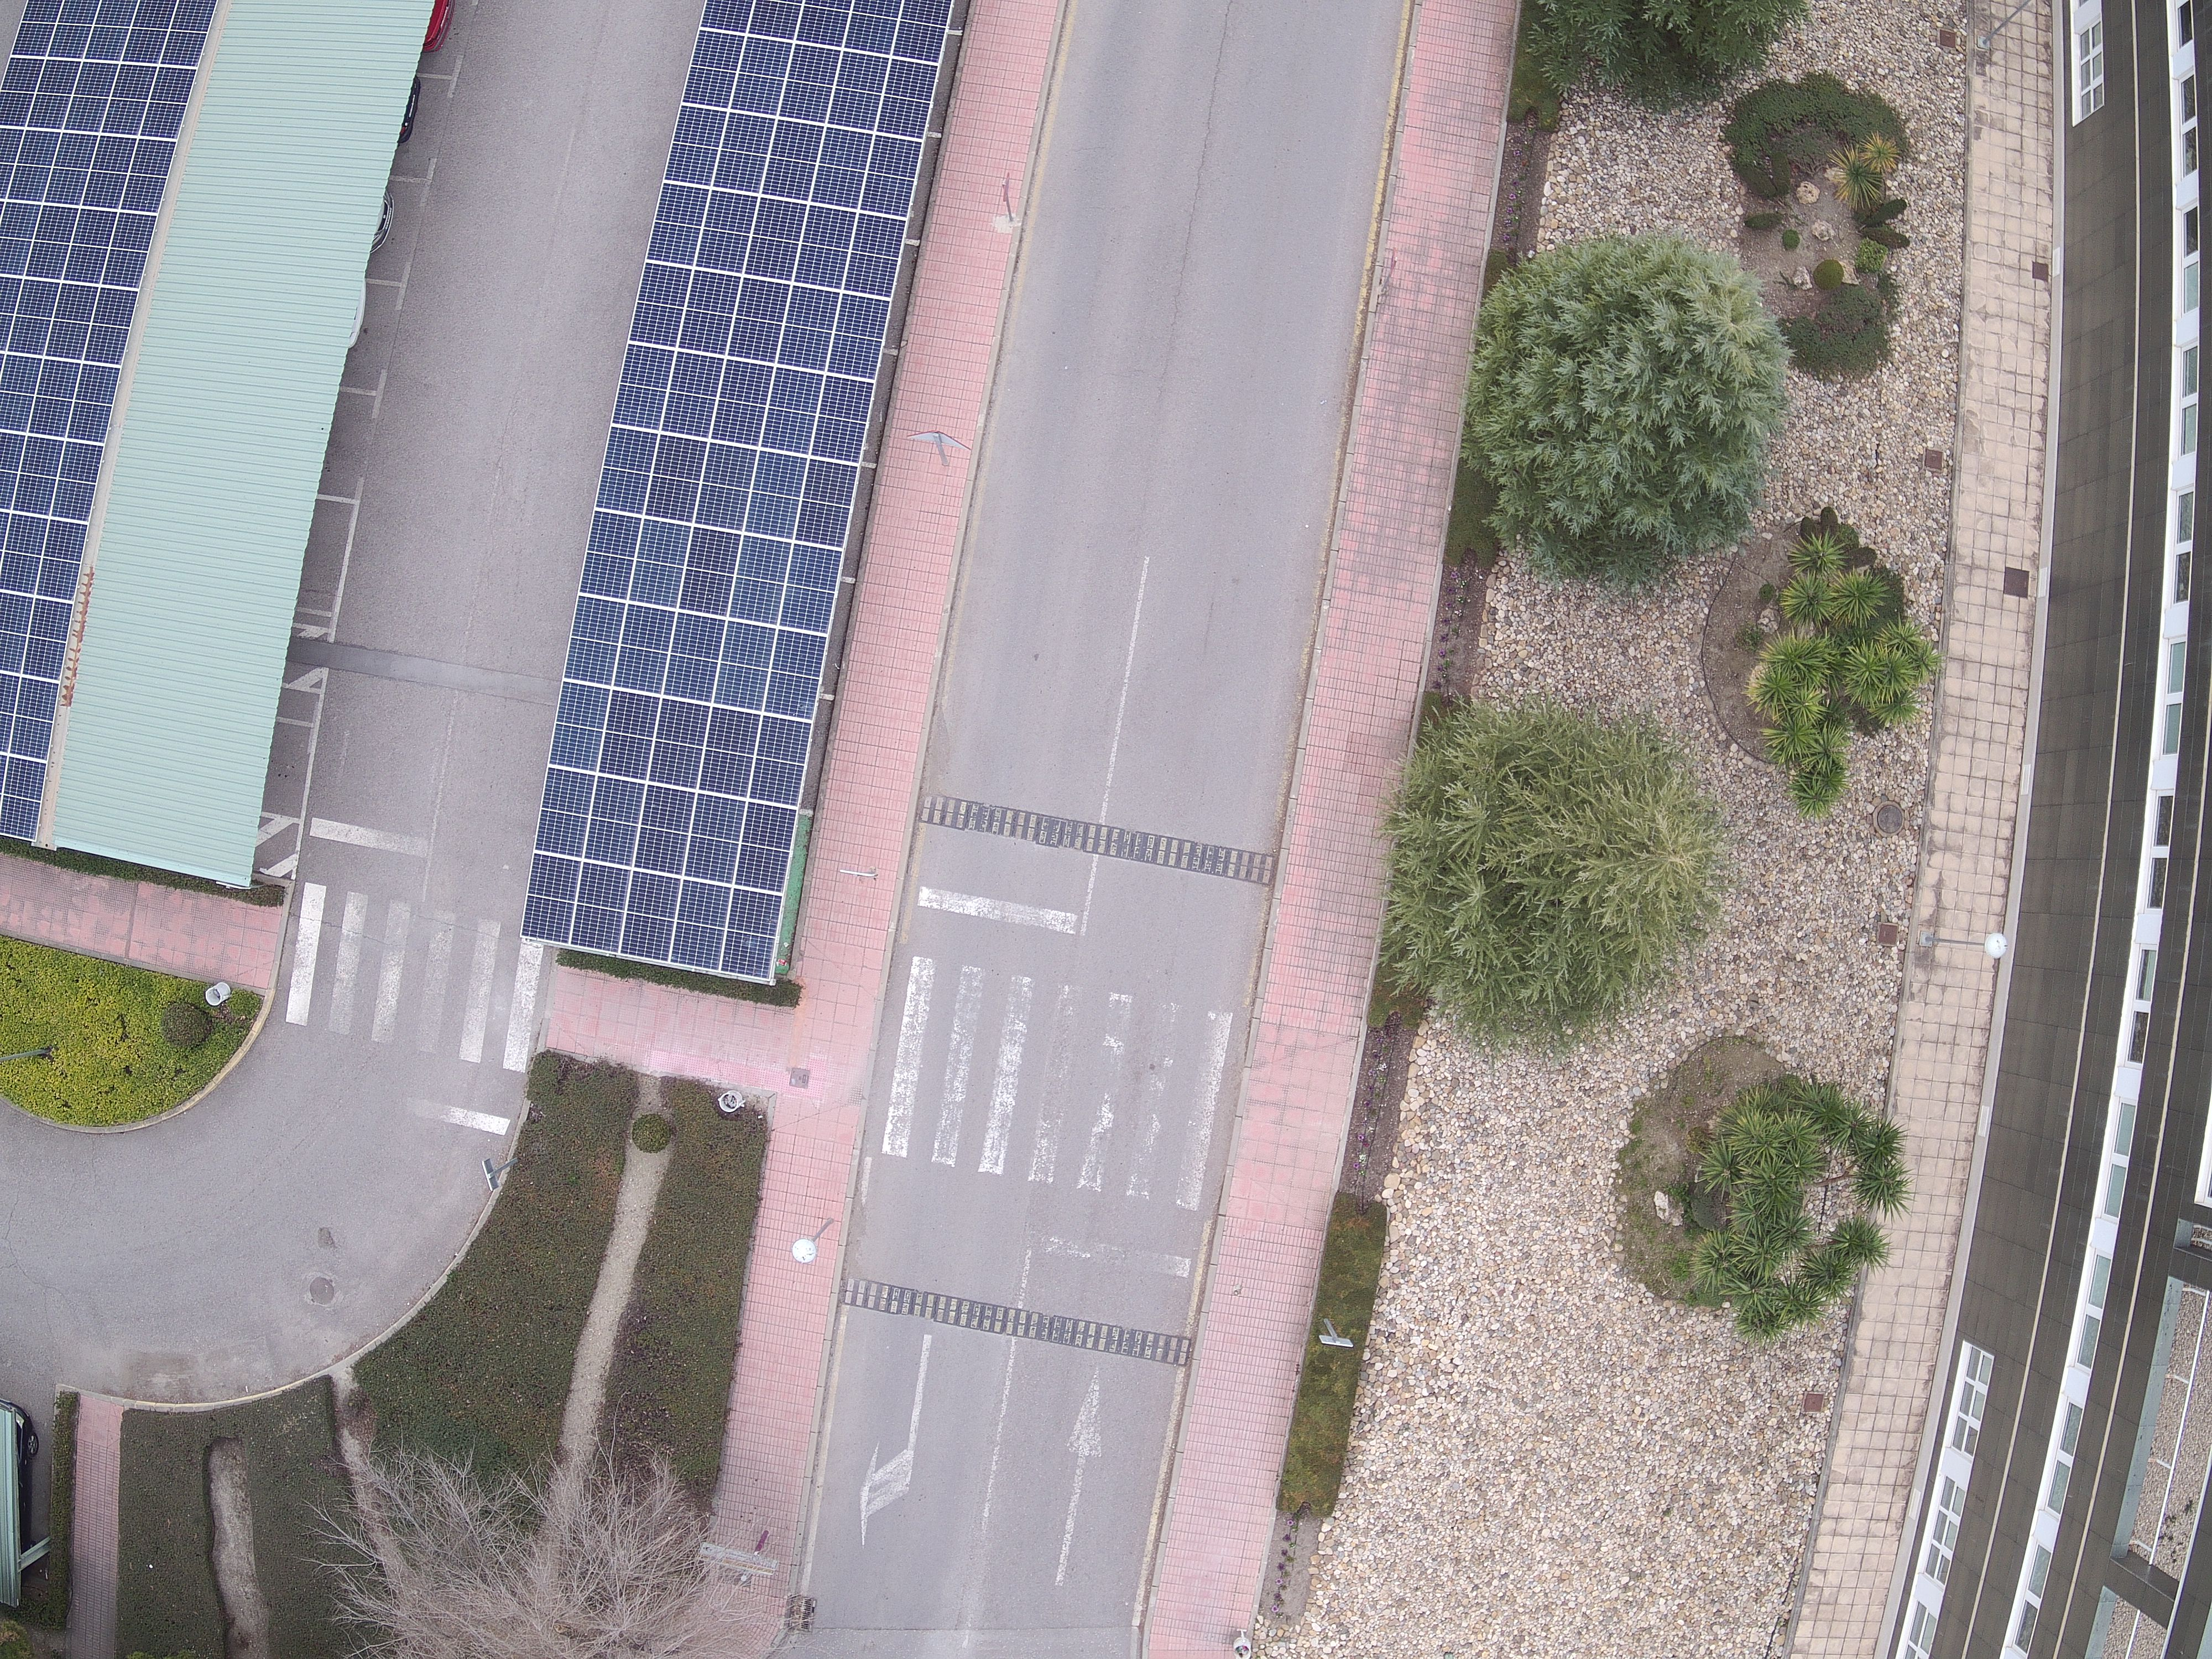
\includegraphics{figs/fundamentals/nadir_image_scan.jpg}
    \caption{Image captured during a flight planned with \textit{nadir} view direction.}
    \label{fig:nadir_image_scan}
\end{marginfigure}

The following sections present the most widespread imaging sensing tools and those that will be covered in the methodology of this work.

\subsection{Multispectral imaging}
\label{sec:multispectral_imaging}

Multispectral images consist of multiple bands corresponding to different wavelengths. However, these are typically discrete readings of spectral intervals with varying bandwidths. Most of the research and academic work describe multispectral as a special case of super spectral and hyperspectral imagery, and so we will, though some remarks are mentioned in this section for our later work. First, Table \ref{table:multispectral_devices} presents some of the multispectral sensors that are frequently revised in the literature, along with the works where they were mentioned. The discrete wavelengths and the resolution of every reading are shown in the fifth column, \textit{Spectral bands}. It can be observed that only a few bands with a coarse resolution, ranging from 14 \si{\micro\meter} to 57 \si{\micro\meter}, are recorded.

\renewcommand{\arraystretch}{1.2}
\begin{table*}[htb]
    \caption{Consumer-grade multispectral devices found in the literature and their specifications, according to the manufacturer's source.}
    \label{table:multispectral_devices}
    \begin{tabular}{llllll}
        \toprule
        Multispectral tool & Focal length & HFOV & Image resolution & Spectral bands (\si{\micro\meter}) & Ref. work \\
        \midrule
        \multicolumn{6}{c}{Parrot}\\
        \cmidrule{1-6}
        \multirow{4}{*}{Sequoia}     & \multirow{4}{*}{3.98 \si{\milli\meter}}   & \multirow{4}{*}{$63.9^{\circ}$}  & \multirow{4}{*}{$1280 \times 960$ px}  & Green: $5.5 \pm 0.2$  & \multirow{4}{*}{\cite{franzini_geometric_2019}}\\
        & & & & Red: $6.6 \pm 0.2$ &\\
        & & & & Red-Edge: $7.35 \pm 0.05$ &\\
        & & & & Near-IR: $7.9 \pm 0.2$ &\\
        \cmidrule{1-6}
        \multicolumn{6}{c}{Micasense}\\
        \cmidrule{1-6}
        \multirow{5}{*}{RedEdge-MX}     & \multirow{5}{*}{5.4 \si{\milli\meter}}   & \multirow{5}{*}{$47.2^{\circ}$}  & \multirow{5}{*}{$1280 \times 960$ px}  & Blue: $4.75 \pm 0.16$     & \multirow{5}{*}{\cite{cunha_prediction_2021, isgro_unmanned_2021}}\\
        & & & & Green: $5.6 \pm 0.13$ &\\
        & & & & Red: $6.68 \pm 0.07$ &\\
        & & & & Red-Edge: $7.17 \pm 0.06$ &\\
        & & & & Near-IR: $8.42 \pm 0.28$ &\\
        \cmidrule{1-6}
        \multirow{10}{*}{Dual-Camera}     & \multirow{10}{*}{5.4 \si{\milli\meter}}   & \multirow{10}{*}{$47.2^{\circ}$}  & \multirow{10}{*}{$1280 \times 960$ px} & Coast blue: $4.44 \pm 0.14$    & \multirow{10}{*}{\cite{chakhvashvili_comparison_2021}}\\
        & & & & Blue: $4.75 \pm 0.16$ &\\
        & & & & Green 1: $5.31 \pm 0.07$ &\\
        & & & & Green 2: $5.6 \pm 0.13$ &\\
        & & & & Red 1: $6.5 \pm 0.08$ &\\
        & & & & Red 2: $6.68 \pm 0.07$ &\\
        & & & & Red-Edge 1: $7.05 \pm 0.05$ &\\
        & & & & Red-Edge 2: $7.17 \pm 0.06$ &\\
        & & & & Red-Edge 3: $7.4 \pm 0.09$ &\\
        & & & & Near-IR: $8.42 \pm 0.28$ &\\
        \cmidrule{1-6}
        \multirow{6}{*}{Altum}     & \multirow{5}{*}{8 \si{\milli\meter}}   & \multirow{5}{*}{$50^{\circ}$}  & \multirow{5}{*}{$2064 \times 1544$ px} & Blue: $5.75 \pm 0.16$    & \multirow{6}{*}{\cite{hutton_high_2020}}\\
        & & & & Green: $5.6 \pm 0.13$ &\\
        & & & & Red: $6.68 \pm 0.07$ &\\
        & & & & Red-Edge: $7.17 \pm 0.06$ &\\
        & & & & Near-IR: $8.42 \pm 0.28$ &\\
        \cmidrule{2-6}
        & \multirow{1}{*}{1.77 \si{\milli\meter}} & \multirow{1}{*}{$57^{\circ}$} & \multirow{1}{*}{$160 \times 120$ px} & Long-Wave IR: $11 \pm 3$ &\\
        \cmidrule{1-6}
        \multirow{6}{*}{Altum-PT}     & \multirow{5}{*}{8 \si{\milli\meter}}   & \multirow{5}{*}{$50^{\circ}$}  & \multirow{5}{*}{$2064 \times 1544$ px} & Blue: $5.75 \pm 0.16$    & \multirow{6}{*}{\cite{hutton_high_2020}}\\
        & & & & Green: $5.6 \pm 0.13$ &\\
        & & & & Red: $6.68 \pm 0.07$ &\\
        & & & & Red-Edge: $7.17 \pm 0.06$ &\\
        & & & & Near-IR: $8.42 \pm 0.28$ &\\
        \cmidrule{2-6}
        & \multirow{1}{*}{1.77 \si{\milli\meter}} & \multirow{1}{*}{$48^{\circ}$} & \multirow{1}{*}{$320 \times 256$ px} & Long-Wave IR: $10.5 \pm 3$ &\\
        \cmidrule{1-6}
        \multicolumn{6}{c}{DJI}\\
        \cmidrule{1-6}
        \multirow{5}{*}{P4 Multispectral}     & \multirow{5}{*}{5.74 \si{\milli\meter}}   & \multirow{5}{*}{$62.7^{\circ}$}  & \multirow{5}{*}{$1600 \times 1300$ px} & Blue: $4.5 \pm 0.08$    & \multirow{5}{*}{\cite{lu_experimental_2020}}\\
        & & & & Green: $5.6 \pm 0.08$ &\\
        & & & & Red: $6.5 \pm 0.08$ &\\
        & & & & Red-Edge: $7.3 \pm 0.08$ &\\
        & & & & Near-IR: $8.4 \pm 0.08$ &\\
        \bottomrule
    \end{tabular}
\end{table*}
\renewcommand{\arraystretch}{1}

\marginnote[3cm]{For tasks such as vegetation classification, visible and near-infrared bands from multispectral imagery are sufficient in most cases. Bare soils tend to show a more constant spectral signature, whereas vegetation presents a steeper slope with higher values in the near-infrared wavelengths \cite{navulur_multispectral_2006}.}
The most frequently recorded bands are Red, Green, Blue, Red-Edge (\acrshort{reg}) and Near-Infrared (\acrshort{nir}), thus overlapping with previous and later imaging tools (visible and thermographic cameras). \acrshort{reg} bands are halfway between Red and \acrshort{nir}, while \acrshort{nir} overlaps with Long-wave Infrared (\acrshort{lwir}) wavelengths. Despite other sensors being able to capture most of these individual bands, multispectral imaging opens a wide number of opportunities by simultaneously recording bands sparsed throughout the visible and infrared spectrum. Most of the multispectral applications benefit from multiple bands through the so-called indices, i.e, linear combinations of them aimed at highlighting relevant features in a group of target objects. In this regard, a total of 82 spectral vegetation indices were collected from the literature by Pu, Ruiliang \cite{pu_hyperspectral_2017}. A recurrent vegetation index in \acrshort{pa} work is the \acrshort{ndvi} (Normalized difference vegetation index), calculated as a combination of Red and \acrshort{nir} bands. Besides identifying vegetation, other indices are focused on estimating pigments and chlorophyll content in plants \cite{pu_hyperspectral_2017}. Most of them work by aggregating bands where the target compound has the most and less significant presence, while others are rather aimed at simply detecting its presence.

\begin{marginfigure}[1.5cm]
    \centering
    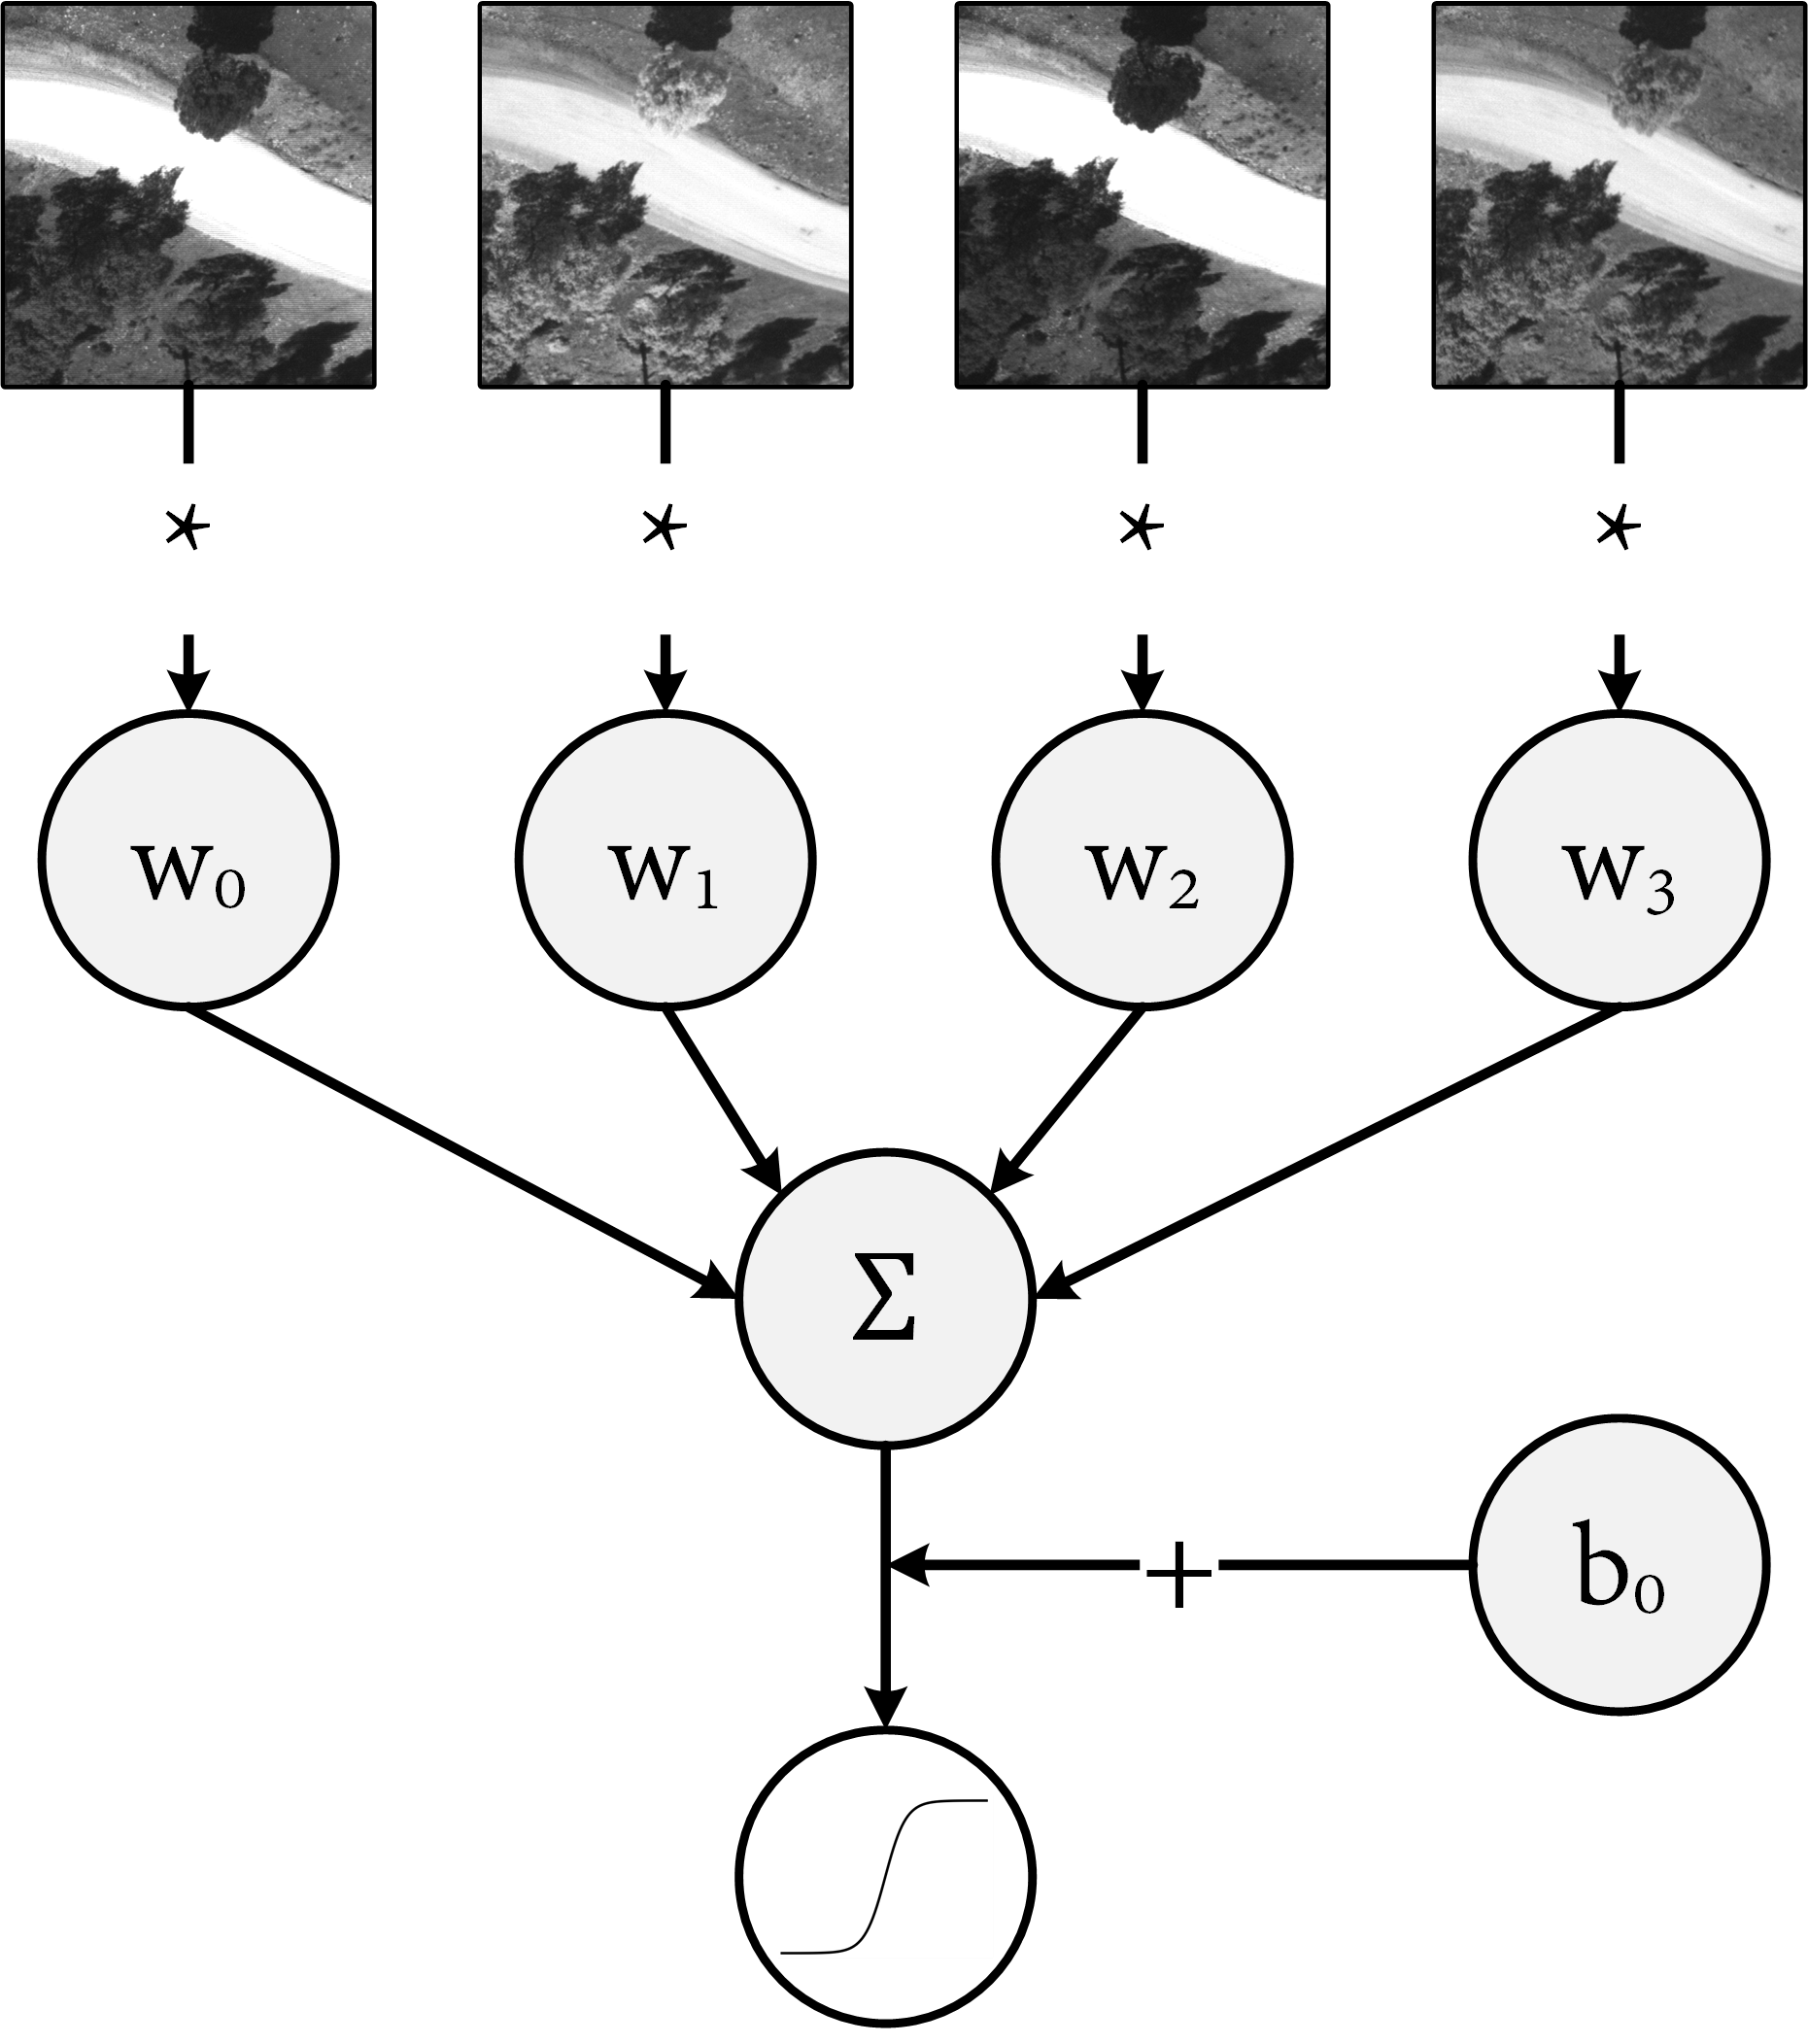
\includegraphics{figs/fundamentals/cnn_ndvi.png}
    \caption{Architecture of a simple neural network with a single layer, aimed at learning the weights of importance of every spectral band.}
    \label{fig:cnn_dvi}
\end{marginfigure}
\begin{kaobox}[frametitle=Activation of relevant spectral bands]
As explained, the aim of spectral indices is to measure or simply indicate the presence of a compound: vegetation, water, etc. A rapid way to determine which bands have a higher weight to highlight a certain compound is to train a trivial neural network with five trainable parameters (Figure \ref{fig:cnn_dvi}). These correspond to four weights ($W^{4\times1}$) belonging to Green, \acrshort{nir}, Red and \acrshort{reg} spectral bands, plus one bias, $b^{1}$. It can be trained over perfectly overlapped multispectral datasets, where the ground truth annotates vegetation and ground. Neither it is a great classifier nor do we plan it to be as so. It was randomly initialized, and the first fitting obtained an overall accuracy close to 98\% and yielded $W = \left[-3.6329935, 33.97777, -67.50758, 2.1926873\right]^{\intercal}$. Hence, \acrshort{nir} and Red bands had a higher contribution to the computed probability, which also happens to correspond to $w_2 \cdot \textit{\acrshort{nir}}$ - $w_3 \cdot \textit{Red}$. \acrshort{ndvi} is, on the other hand, defined in Equation \ref{eq:ndvi}:
\begin{equation}
    \textit{NDVI} = \frac{\textit{NIR} - \textit{Red}}{\textit{NIR} + \textit{Red}}
    \label{eq:ndvi}
\end{equation}
where the aim of $\textit{\acrshort{nir}} + \textit{Red}$ is to normalize the contribution of both spectral bands so that it is minimized when $\lim_{\textit{\acrshort{nir}} \to \textit{Red}} \textit{\acrshort{ndvi}} = 0$ and maximized if $\lim_{\textit{\acrshort{nir}} \to 1 - \textit{Red}} \textit{\acrshort{ndvi}} = 1$, with \acrshort{nir}, Red $\in [0, 1]$. Therefore, the numerator was directly explained by a neural network with a single dense layer, whereas the normalization can be achieved with a simple sigmoid activation, $x \gets w_2 \cdot \textit{\acrshort{nir}}$ - $w_3 \cdot \textit{Red}; s(x) =  \frac{1}{1 + e^{-x}}$, to output a probability $s(x) \in [0, 1]$. It is intended to approximately infer and emulate the $\textit{\acrshort{ndvi}}$ formula; nevertheless, neither $s(x)$ is linear as defined nor the weights were accurately estimated (note that $w_3 > -2 \cdot w_2$).  
\end{kaobox}

However, the revision of vegetation indices converges into the previously mentioned shortcomings of multispectral imagery. Most of these indices operate very specific wavelengths, e.g., 670, 800, 1050, etc., while only a few bands are captured in multispectral imaging. Although it is possible to approximate missing wavelengths with the most similar bands, as shown in Code \ref{code:nearestband}, the results are far from optimal. Therefore, multispectral imaging is better suited for trivial applications such as vegetation classification, while it is not sufficient for other applications that require lower spectral resolution, such as mineral mapping or classifying vegetation species \cite{navulur_multispectral_2006, pu_hyperspectral_2017}. Indeed, most of the metrics proposed in the literature for discerning spectral signatures are based on their derivative. On the other hand, multispectral bands represent a step function with some intervals being undefined.

\vspace{3mm}

\lstinputlisting[language=python, caption={Function for finding the most similar wavelength among those available for a specific sensor data.}, label=code:nearestband]{code/nearest_band.py}

Recently, novel aerial platforms and multispectral sensors are emerging in order to increase the accuracy of spectral measurements, reduce the noise coming from different layers of the atmosphere, and increase the model coverage by multiple view-points with a higher spatial resolution \cite{deng_uav-based_2018}. The \acrshort{uas}’s capabilities to carry lightweight imaging systems have positively impacted recent research. In contrast to satellite images, the \acrshort{gsd} of \acrshort{uas}-multispectral imagery can be significantly reduced to a few centimetres. The increase in spatial resolution and the possibility to capture many overlapped images enable the development of image-based techniques for 3D model reconstruction.

Finally, remark that the processing of multispectral imagery from commercial devices is performed with proprietary software and formulae defined by manufacturers. The acquired irradiance at discrete wavelengths is not transformed in a manner that involves the spectral signature. Instead, irradiance is typically turned into reflectance using the shutter speed, the observation angle, the gain factor and other calibration coefficients, either provided by the manufacturer or obtained before and after flights \cite{jurado_semantic_2020, candiago_evaluating_2015}.

\subsection{Thermography}
\label{sec:thermography_imaging}

\begin{marginfigure}[1cm]
    \centering
    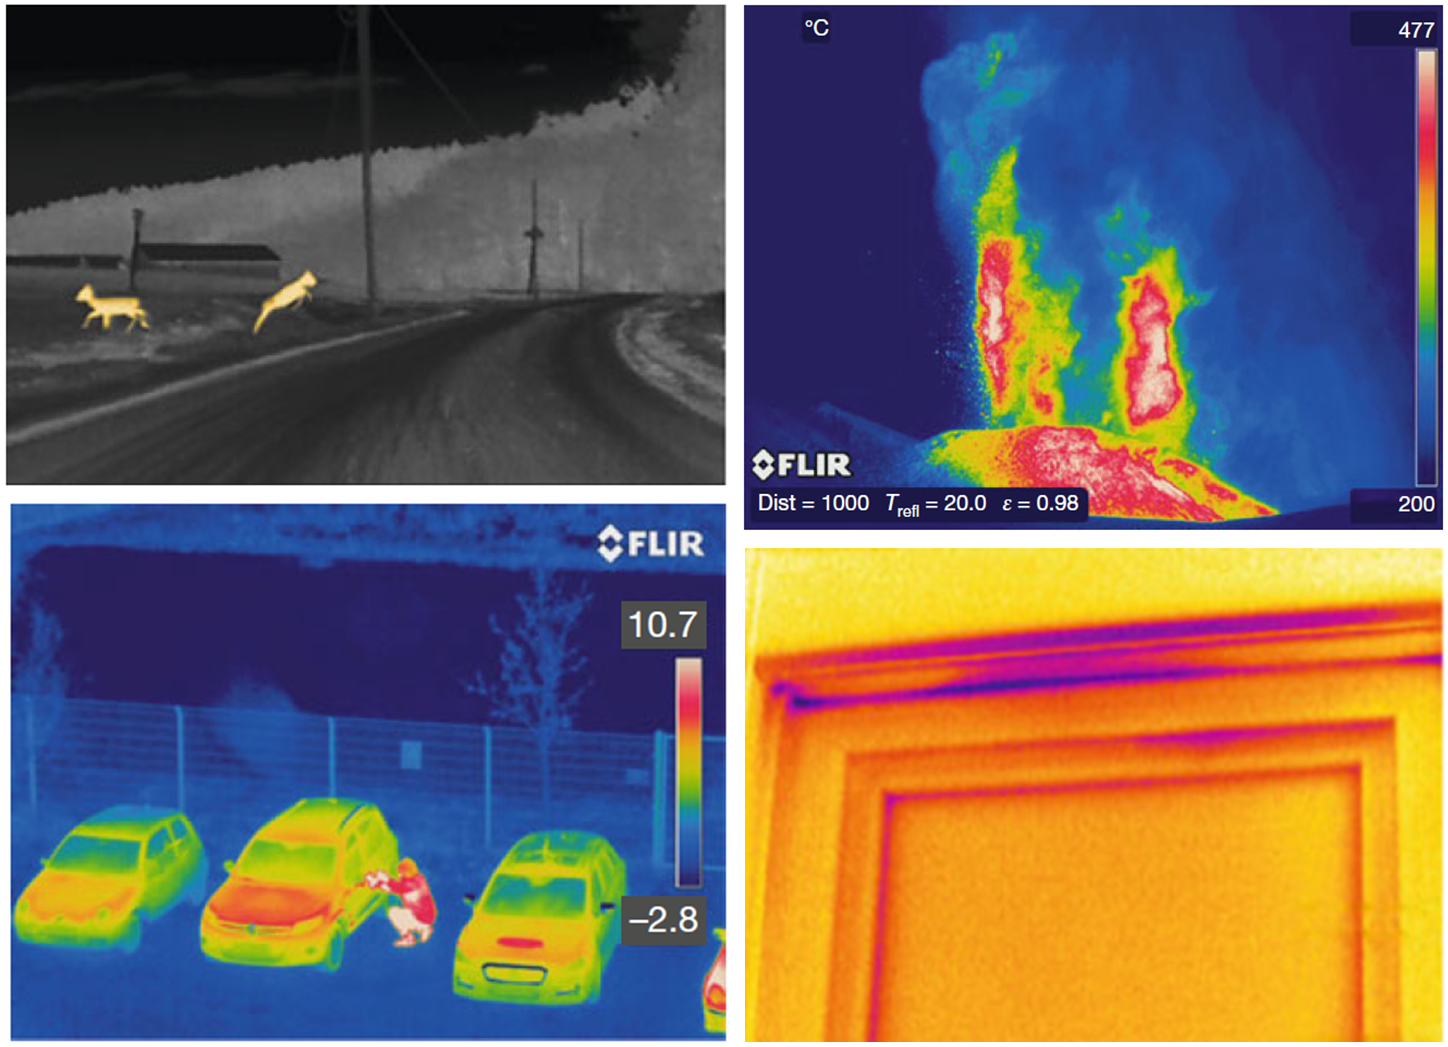
\includegraphics{figs/fundamentals/thermal_applications.png}
    \caption{Some applications of infrared imaging \cite{vollmer_infrared_2017}. From left to right, and from top to bottom: night vision, volcano monitoring, surveillance and detection of incorrect thermal insulation.}
    \label{fig:thermal_applications}
\end{marginfigure}
Infrared thermal imaging (\acrshort{ir}) or thermography is a noninvasive technology for acquiring the temperature of objects' surfaces and phenomena through their emitted radiation. In recent years, rapid growth has been witnessed due to the progress made in the technology of infrared detectors. Furthermore, the competition among camera manufacturers has led to releasing low-cost \acrshort{ir} products, thus widening the applicability scope and diversity of customers. It is considered an excellent noninvasive technology, and therefore, it is applied over very different scopes. Some of the most revised applications in the literature are quality control and monitoring in industrial environments \cite{alfredo_osornio-rios_recent_2019, vollmer_infrared_2017}, medical analysis \cite{lorinczy_thermal_2017}, building inspection \cite{jarzabek-rychard_supervised_2020, kylili_infrared_2014}, agriculture and animal applications \cite{mcmanus_infrared_2016, tsouros_review_2019}, geological monitoring \cite{grechi_3d_2021}, fire and gas leaks detection \cite{gade_thermal_2014}, surveillance, etc. (see Figure \ref{fig:thermal_applications}). On crop and forest management, it has been mainly applied to tree characterization by measuring their energy flux, evapotranspiration and photosynthesis \cite{webster_three-dimensional_2018}, as well as for water stress and disease detection \cite{yandun_narvaez_survey_2017, de_oca_uas_2021, zarco-tejada_previsual_2018}. Heating monitoring also prevents frost damage from crops \cite{yuan_uav-based_2021}. 

\begin{marginfigure}[.15cm]
	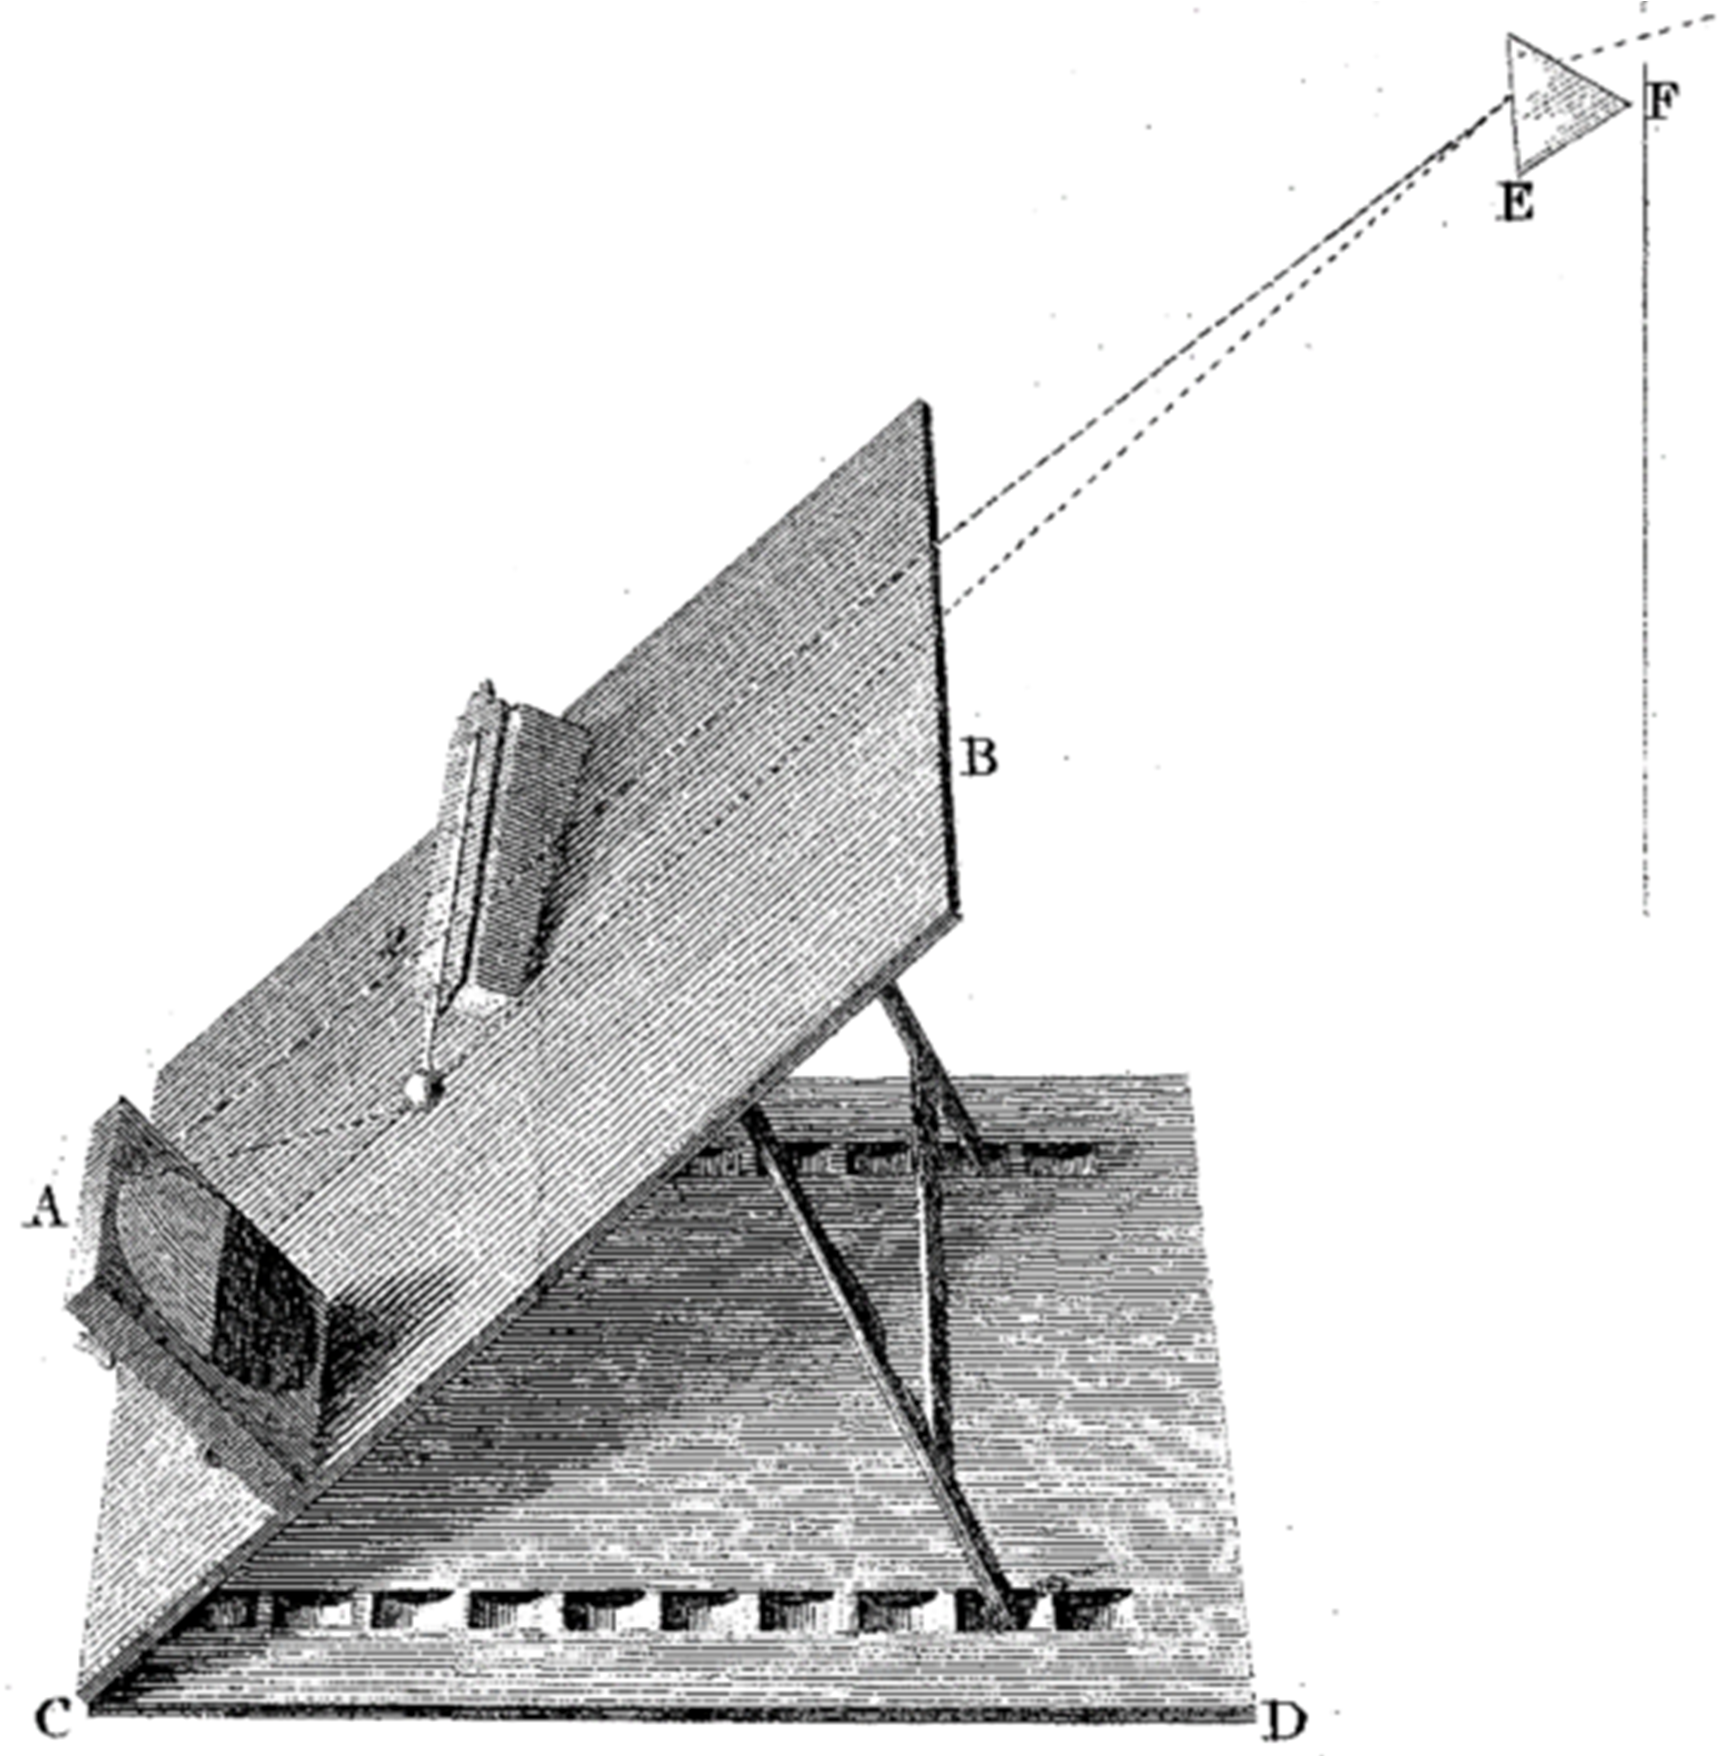
\includegraphics{figs/fundamentals/herschel_decomposition.png}
	\caption{Measurement stand for reading temperature from radiation with a single thermometer \cite{minkina_how_2021}.}
	\label{fig:herschel_decomposition}
\end{marginfigure}
\begin{marginfigure}[7cm]
	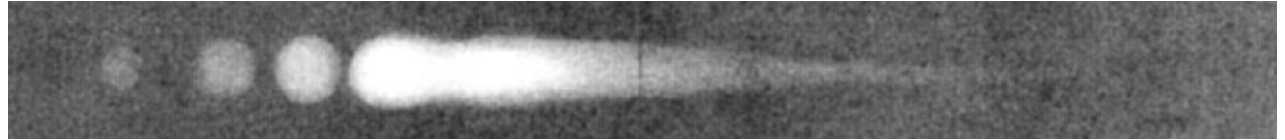
\includegraphics{figs/fundamentals/infrared_absorption.png}
	\caption{Example of thermogram originated from a wet piece of paper and targetted radiation.}
	\label{fig:infrared_absorption}
\end{marginfigure}
\begin{kaobox}[frametitle=Discovery of infrared radiation]
The heat was initially believed to only transfer through matter until the experiments of William Herschel led to the discovery of 'calorific' or 'invisible' rays. This term referred to wavelengths that fall beyond the red spectral interval end and thus are invisible to the naked eye. Circa 1737, Châtelet suggested that different colours could carry different temperatures, though it would not be until 1800 that this theory was proved. W. Herschel passed the Sun's radiation through a prism and placed mercury thermometers over the split spectrum. The measured temperatures not only differed from atmospheric temperature but also the readings beyond the red end were higher. A more advanced set-up of this experiment is shown in Figure \ref{fig:herschel_decomposition}, with a reflective mirror and a platform that can vary its slope \cite{ring_discovery_2000, minkina_how_2021, minkina_infrared_2009}. Later in 1804, John Leslie checked the discrepancies in the temperature readings of different materials, using the so-called Leslie cube. Another curious experiment showed that there exist atmospheric windows with a higher transmission factor and less absorption. W. Herschel's son, John Herschel, used the technique called evaporography to create a thermal image, also known as a thermogram, over a wet piece of paper. The result is shown in Figure \ref{fig:infrared_absorption}, with white dots representing beyond infrared wavelengths. 
\end{kaobox}

\acrshort{ir} radiation is physically represented as electromagnetic (\acrshort{em}) waves that propagate through space as a sinusoidal function ($f(x) = k \cdot \sin{x}$) with a spatial periodicity, known as wavelength (\si{\meter}), $\lambda$, and a period of oscillation (\si{\second}), $\mathcal{T}$. 
%The speed of propagation depends on the kind of wave and is calculated with the frequency $\nu$ derived from $\mathcal{T}$ and $\lambda$. However, EM waves are known to propagate at the speed of light ($c = 300 000\si{\kilo\meter}^{-1}$) in a vacuum; otherwise, $c$ depends on the index of refraction of the medium of propagation. 
Waves are affected by disturbance, and according to this can be organized into longitudinal and transverse waves, with both being perpendicular. Transverse waves can oscillate in many different directions, which yields the concept of polarization and plane of polarization. The latter is defined through the direction of propagation and the disturbance. If a wave is categorized as unpolarized, then the plane of polarization can adopt all possible orientations. Regarding \acrshort{ir} radiation, it is perturbed by electric and magnetic fields, and its polarization is expressed through the electric field and the direction of propagation ($x-z$ plane). Therefore, the recording of waves and \acrshort{ir} radiation can be performed by polarizers, with a simple microscopically small conducting grid being sufficient for filtering out waves that are non-perpendicular to such a grid \cite{vollmer_infrared_2017}. In thermography, the captured \acrshort{em} radiation is referred to \textbf{thermal radiation}, emitted by bodies at a temperature over 0 \si{\kelvin} (-273.15ºC). 

The radiation measured from a surface is not solely affected by such a surface, but other factors intervene in the acquisition. Among these, the most notable factors are the absorption and scattering phenomena from atmospheric particles and sensor components, as well as the radiation emitted by surrounding objects and the atmosphere. The degree of transmissivity of the atmosphere, which may vary throughout time, is known as the transmission factor. Other minor influencing factors are the distance to the sensor, the object's emissivity, dimensions and shape, the atmospheric temperature and humidity as well as the temperature of optics \cite{vollmer_infrared_2017}. 

Although the \acrshort{ir} spectrum covers a wide range of wavelengths (see Figure \ref{fig:introduction_scheme}), \acrshort{ir} imaging is focused on a small part of these. Three spectral ranges are the most frequent in thermography: short-wave infrared (\acrshort{swir}: 900-1,700 \si{\nano\meter}), mid-wave infrared (\acrshort{mwir}: 3,000-5,000 \si{\nano\meter}) and long-wave infrared (\acrshort{lwir}: 8,000-14,000 \si{\nano\meter}) \cite{gade_thermal_2014, vollmer_infrared_2017}. Commercial sensors are available on the three spectral ranges; whether one of them ought to be used over another must attend to criteria such as atmospheric transmission, expected radiation and the physics of detectors. A simple Scopus search shows that \acrshort{mwir} imaging is the most widespread, though it is significantly downgraded over \acrshort{swir} and \acrshort{lwir} for \acrshort{uas} platforms. Figure \ref{fig:infrared_scopus} shows the percentage of work devoted to each \acrshort{ir} interval. The Scopus searches were the following: $(\mathtt{thermographic} \lor \mathtt{thermography} \lor \mathtt{thermal} \lor \mathtt{infrared} \lor \mathtt{ir}) \land (\mathtt{drone} \lor \mathtt{uav} \lor \mathtt{uas}) \land ((x-\mathtt{wave} \lor y\mathtt{WIR}))$, with $x$ being short ($y \gets $S), mid ($y \gets $M) or long ($y \gets $L). In this dissertation, the integrated thermographic camera operates over the \acrshort{lwir} range. 

\begin{figure}[ht]
	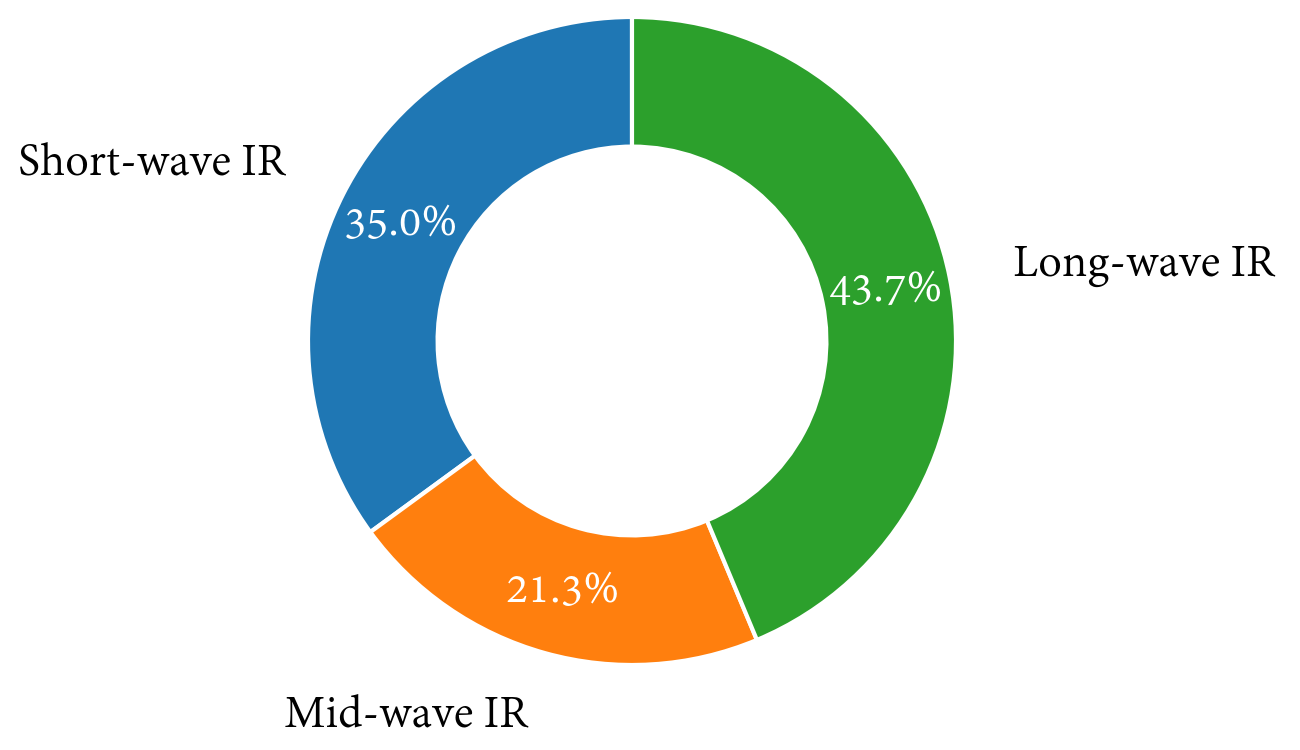
\includegraphics[width=.75\textwidth]{figs/fundamentals/infrared.png}
	\caption{Number of manuscripts related to different \acrshort{ir} intervals.  }
    \label{fig:infrared_scopus}
\end{figure}

Preferences on the \acrshort{lw} range over \acrshort{swir} and \acrshort{mwir} are not a casualty, but it is rather influenced by atmospheric transmissivity. Most of Earth's surface has its emission peak in this interval, while the \acrshort{lw} range is also known as an atmospheric window where absorption is considerably smaller \cite{gonzalez_thermal_2019, quattrochi_thermal_1999}. 

An exhaustive, though not complete, list of the most frequent commercial \acrshort{ir} cameras used for research is shown in Table \ref{table:thermographic_devices}. Every single of them is designed for measuring \acrshort{lwir}, while their focal length is typically over 13 \si{\milli\meter}. Instead of widening the camera view, these devices acquire images focused on very specific areas with a very small image resolution. Therefore, the mentioned drawbacks ought to be considered to make an appropriate flight plan. For instance, side overlapping among different sweeps from the planned trajectory must be large enough to guarantee there exists overlapping between thermal imagery. 

\renewcommand{\arraystretch}{1.2}
\begin{table*}[htb]
    \small
    \caption{Consumer-grade thermal devices found in the literature and their specifications, according to the manufacturer's datasheets.}
    \label{table:thermographic_devices}
    \begin{tabular}{llllll}
        \toprule
        Thermographic tool & Focal length & FOV & Image res. & Spectral range & Ref. work \\
        \midrule
        \multicolumn{6}{c}{DJI}\\
        \multirow{2}{*}{Zenmuse XT2}    & 13 \si{\milli\meter}   & $32^{\circ} \times 26^{\circ}$  & $640 \times 512$ px  & \multirow{2}{*}{LWIR (7.5 - 13.5 \si{\micro\meter})}    & \multirow{2}{*}{\cite{lopez_optimized_2021, yuan_uav-based_2021, jo_dense_2021}}\\
        & 19 \si{\milli\meter}   & $25^{\circ} \times 19^{\circ}$  & $336 \times 256$ px  &   & \\
        Zenmuse H20T     & 13.5 \si{\milli\meter}   & $31.7^{\circ} \times 25.36^{\circ}$  & $640 \times 512$ px  & LWIR (8 - 14 \si{\micro\meter})    & \cite{paziewska_integration_2022, jiang_diurnal_2022}\\
        \cmidrule{1-6}
        \multicolumn{6}{c}{FLIR}\\
        FLIR A320     & 18 \si{\milli\meter}   & $25^{\circ} \times 18.8^{\circ}$  & $320 \times 240$ px  & LWIR (7.5 - 13.5 \si{\micro\meter})    & \cite{guilbert_fusion_2020}\\
        FLIR A35     & 9 \si{\milli\meter}   & $48^{\circ} \times 39^{\circ}$  & $320 \times 256$ px  & LWIR (7.5 - 13.5 \si{\micro\meter})    & \cite{comba_2d_2019}\\
        FLIR One     & 15 \si{\centi\meter}   & $50^{\circ} \times 38^{\circ}$  & $80 \times 60$ px  & LWIR (8 - 14 \si{\micro\meter})    & \cite{javadnejad_photogrammetric_2020}\\
        FLIR A65     & 25 \si{\milli\meter}   & $25^{\circ} \times 20^{\circ}$  & $640 \times 512$ px  & LWIR (7.5 - 13.5 \si{\micro\meter})    & \cite{adan_fusion_2017, jarzabek-rychard_supervised_2020, lin_fusion_2019, westfeld_generation_2015}\\
        FLIR Tau2 640     & 13 \si{\milli\meter}   & $45^{\circ} \times 37^{\circ}$  & $640 \times 512$ px  & LWIR (7.5 - 13.5 \si{\micro\meter})    & \cite{boesch_thermal_2017, sledz_thermal_2018}\\
        \cmidrule{1-6}
        \multicolumn{6}{c}{Sensefly}\\
        Sensefly thermoMAP     & N.A.   & N.A.  & $640 \times 512$ px  & LWIR (7.5 - 13.5 \si{\micro\meter})    & \cite{padua_vineyard_2019}\\
        \bottomrule
    \end{tabular}
\end{table*}
\renewcommand{\arraystretch}{1}

\subsection{Hyperspectral imaging}

Hyperspectral imaging (\acrshort{hsi}) differs from multispectral imaging in the number of bands, wavelengths and bandwidth of these. Hyperspectral images are 3D data cubes known as \textbf{hypercubes}, where each pixel is defined within a continuous spectrum range (Figure \ref{fig:fundamentals_material_hyperspectral}). The spectral resolution is typically given in \si{\nano\meter} or as a number of bands, though the second is preferred as the resolution can vary throughout the covered interval. Spectral signatures are complete and differentiable over the observed wavelength range, and thus, hypercubes outperform discrete multispectral data on the classification, segmentation and unmixing of materials. For instance, different varieties of plants might have a radiative response too similar among them, even using \acrshort{hsi}. Therefore, \acrshort{ai} algorithms could be applied to the automatic detection of the most discriminative wavelengths and be accordingly weighted to provide a meaningful result from input data. 

Unlike other imaging tools, \acrshort{hsi} has undergone a rising path from major to minor; from satellite scanning to \acrshort{uas} and laboratory applications. Hence, it is applied in a wide range of applications, from phenotyping, cultural heritage, medical research and food processing to biochemistry and the monitoring of Earth's processes and areas of interest, among others \cite{amigo_hyperspectral_2019}. Also in contrast to multispectral imaging, preprocessing on \acrshort{hsi} is still very frequently investigated. 

Remotely sensed data is affected by several factors, including acquisition conditions and random errors caused by sensors as well as atmospheric and surface effects. Radiometric correction over \acrshort{hsi} has been conducted to obtain representative data from the Earth's surfaces. The bibliography on this field has covered many topics, though it is mainly focused on satellite imaging. While some of the studied techniques can be applied to \acrshort{uas} imaging, other chapters are irrelevant to our target platforms, \acrshort{uas}. For instance, atmospheric effects such as absorption are of no interest in close-range work. However, the low flight altitude, the \acrshort{uas} instability or its viewing angle harden the pre-processing operations \cite{jakob_need_2017}. Geometric and radiometric corrections as well as spectral calibrations are also required to obtain accurate data \cite{adao_hyperspectral_2017}. Geometric distortions refer to those defects caused primarily by the \acrshort{uas} instability as well as due to the acquisition technique. For instance, push-broom sensors present higher geometric distortions that can be reduced by means of stabilizers. Geometric correction can be achieved with an \acrshort{imu}, a \acrshort{gps} as well as a Digital Elevation Model (\acrshort{dem}). Although there exists commercial software based on this approach, it requires a high-precision system for obtaining accurate corrections. Instead, Ground Control Points (\acrshort{gcp}) have been extensively used to ensure correct positioning \cite{ramirez-paredes_low-altitude_2016}. Also, the dual acquisition of visible and hyperspectral imagery allows matching both data sources \cite{jurado_efficient_2021, xue_compact_2021, ramirez-paredes_low-altitude_2016}, with the visible data being geometrically correct. Alternatively, feature matching among overlapping images has also been shown to help with geometric correction \cite{akhoundi_khezrabad_new_2022}.

\begin{figure}[ht]
	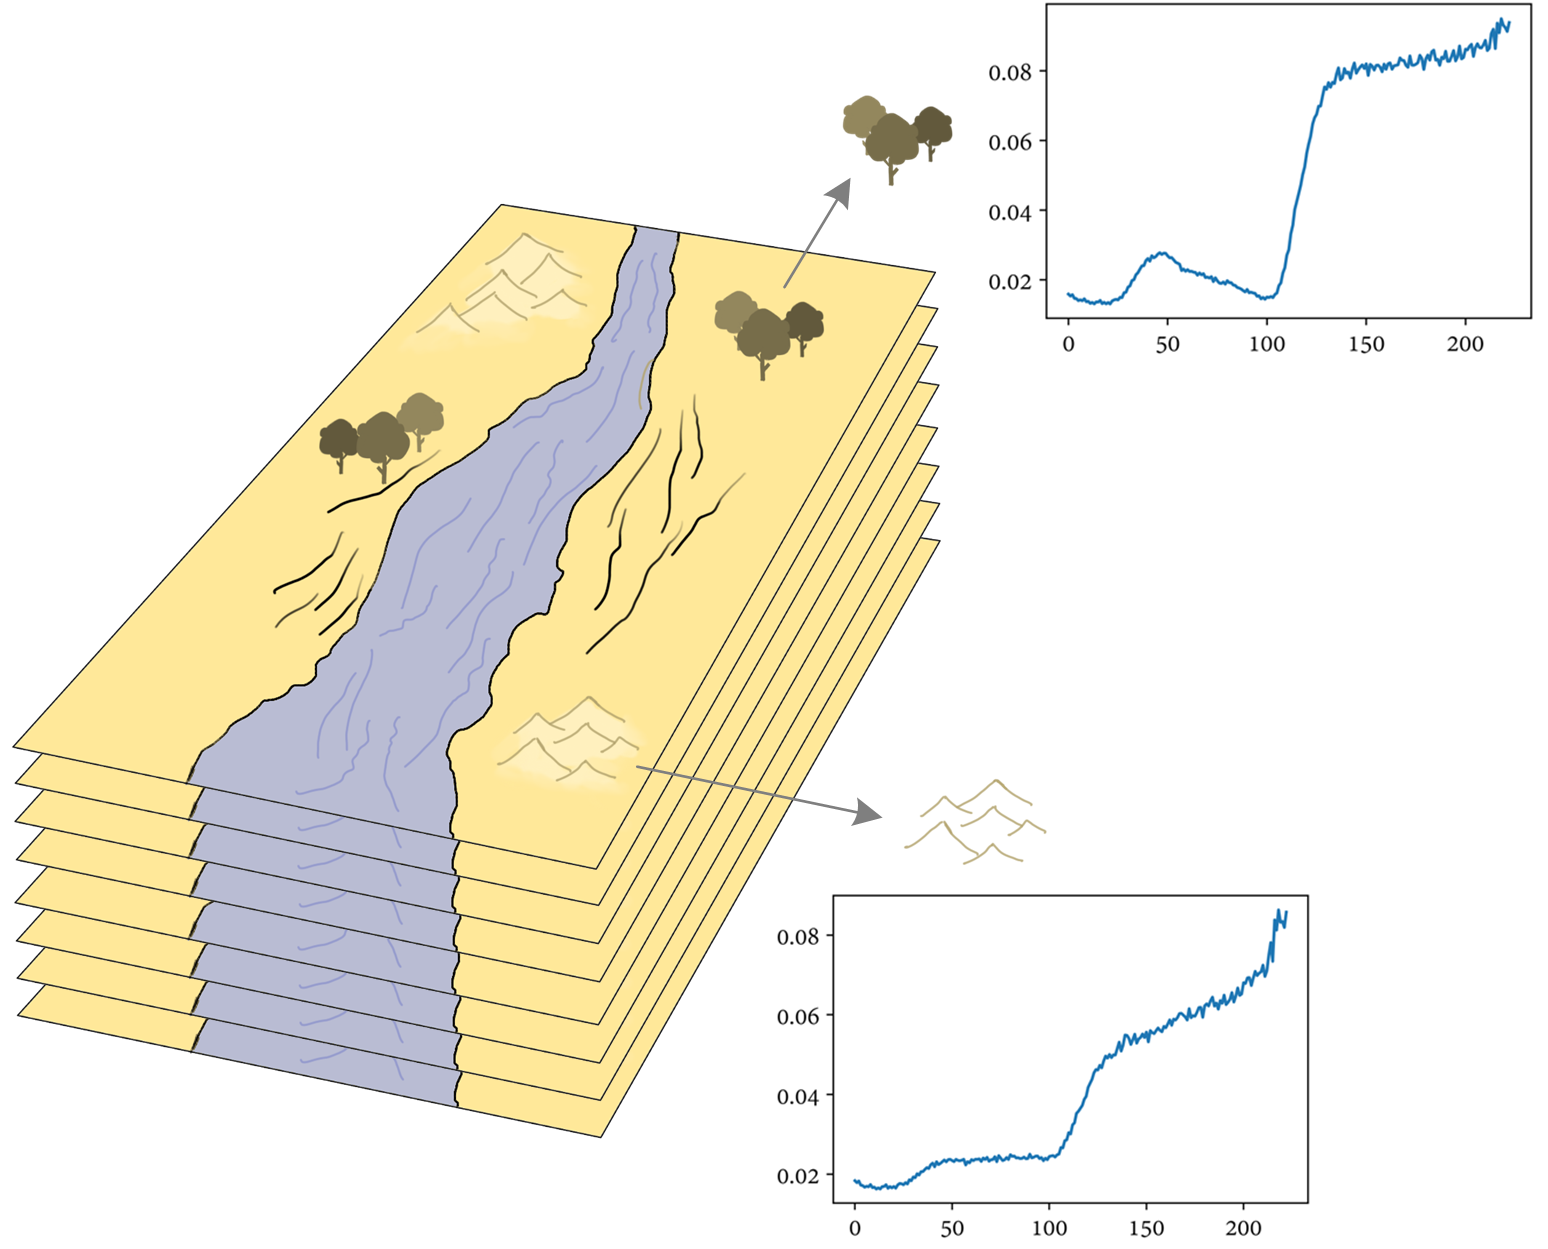
\includegraphics[width=.9\textwidth]{figs/fundamentals/material_hyperspectral.png}
	\caption{Scheme of hyperspectral images, where vegetation and ground surfaces have a different spectral signature.  }
    \label{fig:fundamentals_material_hyperspectral}
\end{figure}

Similarly to geometric distortions, radiometric defects can be corrected with software tools from the hyperspectral manufacturer. The objective is to transform the sensor's \acrshort{dn} to radiance, influenced by acquisition conditions, and reflectance, regardless of previous conditions. To this end, the coefficients needed for this correction are typically calibrated in the laboratory. However, they are more likely to vary through time \cite{adao_hyperspectral_2017}, thus leading to worsening the radiometric correction. This process can be supported by the use of grayscale tarps whose reflectance is known, thereby allowing to perform linear interpolations to calibrate the acquired \acrshort{dn} \cite{lucieer_hyperuasimaging_2014} with the Empirical Line Method (\acrshort{elm}) \cite{aasen_quantitative_2018, sousa_uav-based_2022}. Dark and grey/white references are required to perform this linear interpolation \cite{jakob_need_2017, sagan_data-driven_2022, duan_land_2013}, typically from isotropic materials (near to Lambertian) that present a grayscale palette. Alternatively, the acquisition of radiance samples can help to transform \acrshort{dn}s with fitting methods such as the Least-Square Method (\acrshort{lsm}). Sensor-based factors, including the vignetting effect that causes a drop in the intensity, lead to a different radiometric response in pixels of the same bands \cite{yang_dom_2017}.

Atmospheric corrections have also been documented for \acrshort{uas} flights. Accordingly, the at-sensor radiance can be correlated to the surface Hemisphe\\rical-Directional Reflectance Function (\acrshort{hdrf}) measured in the laboratory beforehand. The previous grayscale palette with Lambertian materials can be used to achieve this \cite{lucieer_hyperuasimaging_2014}. Physically-based methods have also been investigated by measuring the atmospheric conditions that conditioned the hyperspectral imaging, though they are more time-consuming. Finally, some public repositories offer atmospherically corrected datasets, e.g., the Aviris data portal \cite{california_institute_of_technology_aviris_nodate}, whereas widespread software for hyperspectral processing also includes semi-automatic correction algorithms (ENVI, Headwall SpectralView, etc). Other studies calculate the Bidirectional Reflectance Distribution Function (\acrshort{brdf}) of visible materials. Previous corrections are applied, and \acrshort{brdf} kernels are estimated using kernels such as Ross and Li from the varying response of materials according to solar and view angles \cite{queally_flexbrdf_2022, jia_kernel-driven_2020, sagan_data-driven_2022}.

The list of hyperspectral sensors on the market that can be coupled with \acrshort{uas} has significantly increased in recent years. Therefore, Table \ref{table:hyperspectral_devices} solely illustrates those that provide higher spectral resolution and have been explored in the hyperspectral state-of-the-art literature. As previously regarded, the spectral range can be calculated from the spectral resolution, in \si{\nano\meter}, and the number of bands. However, as observed in Table \ref{table:hyperspectral_devices}, this is not exactly right for every sensor as the spectral resolution may not be constant. In this dissertation, the research focused on hyperspectral imaging operates over data cubes from Headwall Photonics Inc.\textregistered Nano HyperSpec, with sampling intervals ranging from 2.2 \si{\nano\meter} to 6 \si{\nano\meter} in the central wavelengths.

\renewcommand{\arraystretch}{1.2}
\begin{table*}[h]
    \small
    \caption{Hyperspectral sensors found in the literature and their specifications, according to the manufacturer's datasheets.}
    \label{table:hyperspectral_devices}
    \begin{tabular}{lllllll}
        \toprule
        Tool & Spectral range & \#Bands & Spectral res. & Acquisition & Spatial res. & Ref. work \\
        \midrule
        \multicolumn{7}{c}{Headwall Photonics}\\
        Nano HyperSpec & 400-1000 \si{\nano\meter}   & 272-775 & 6 \si{\nano\meter}  & Push-broom    & 640 px  &\cite{sankey_uav_2018, sousa_uav-based_2022}\\
        Micro Hyperspec & 400-1000 \si{\nano\meter}   & 837-923 & 2.5 \si{\nano\meter}  & Push-broom    & 1004 px  &\cite{sousa_uav-based_2022}\\
        \cmidrule{1-7}
        \multicolumn{7}{c}{SENOP}\\
        VIS-VNIR Snapshot & 400-900 \si{\nano\meter}   & 380 & 10 \si{\nano\meter}  & Snapshot    & $1010\times1010$ px & \cite{sousa_uav-based_2022}\\
        HSC-2 & 450-900 \si{\nano\meter}   & Up to 1000 & 6-18 \si{\nano\meter}  & Snapshot    & $1024\times1024$ px & \cite{sousa_uav-based_2022}\\
        \cmidrule{1-7}
        \multicolumn{7}{c}{XIMEA}\\
        XIMEA SNm4x4 & 460-600 \si{\nano\meter}   & 16 & 15 \si{\nano\meter}  & Snapshot    & $512\times272$ px & \cite{gao_cbff-net_2023}\\
        \cmidrule{1-7}
        \multicolumn{7}{c}{Specim}\\
        AISA Angle & 400-970 \si{\nano\meter}   & 488 & 2.9 \si{\nano\meter}  & Pushbroom    & $1024$ px & \cite{windrim_unsupervised_2023}\\
        FX17 & 900-1700 \si{\nano\meter}   & 224 & 8 \si{\nano\meter}  & Pushbroom    & $640$ px & \cite{sousa_uav-based_2022}\\
        \cmidrule{1-7}
        \multicolumn{7}{c}{Cubert GmbH}\\
        UHD 185 Firefly & 450-950 \si{\nano\meter}   & 125 & 8 \si{\nano\meter}  & Snapshot    & $1000\times1000$ px & \cite{yue_comparison_2018}\\
        \bottomrule
    \end{tabular}
\end{table*}
\renewcommand{\arraystretch}{1}

\subsection{Active sensing}

Active systems, unlike previous passive sensors, provide their own energy source and therefore do not rely on external light sources, radiation emitted and reflected by surfaces and weather conditions \cite{dong_lidar_2018}. Among active sensors, the focus of this dissertation is on \acrshort{lidar}. It is an optical remote sensing technique that measures the properties of scattered light and can be used on spaceborne, airborne and ground-based platforms. The emitted energy is bounced back after colliding on the Earth's surfaces, thus being capable of determining distances by measuring the time delay between emission and reception, the so-called Time of Flight (\acrshort{tof}). It is also aimed at measuring speed (wind \acrshort{lidar}) and attenuation of volume targets such as the atmosphere or seawater \cite{emery_introduction_2017}. The emitted electromagnetic energy operates at a wavelength, with \acrshort{lidar} working at much shorter wavelengths than radar, typically in atmospheric transmission windows. Some of these were previously reviewed (infrared), although \acrshort{lidar} systems also operate at the visible and ultraviolet (\acrshort{uv}) spectral range. This parameter determines which is the minimum size of objects to be detected, with shorter wavelengths being more sensitive to smaller particles. Hence, \acrshort{lidar} systems are typically used for atmospheric and meteorology research. Backscattering is dependent on the dielectric discontinuity produced by collided surfaces, and therefore, nonmetallic objects have significantly lower responses to higher wavelengths \cite{dong_lidar_2018}. 

A simplification of \acrshort{lidar} emissions is the concept of ray: $r(t) = o + \vec{d}t$. This is a geometric data type defined by the starting position, $o$, and a direction vector, $\vec{d}$, that infinitely spread in the space. Unlike rays in Computer Graphics (\acrshort{cg}), \acrshort{lidar} emit volumetric beams whose targets are surface areas rather than points. Therefore, impacts on surfaces may not entirely block these beams, thus leading to penetrating surfaces that harden the visualization of objects below it but are not completely enclosed. For example, \acrshort{lidar} has been applied to archaeology with notable results since it allows removing points from high-density forests to uncover remains at the Earth's surface. Other widespread applications of \acrshort{lidar} technology are in \acrshort{rs}, geology, atmospheric physics or seismology \cite{emery_introduction_2017}. More specific ones concerning our work are building inspections \cite{shariq_revolutionising_2020}, monitoring of natural environments (landform dynamics \cite{guisado-pintado_3d_2019}, ecological resilience \cite{mitasova_geospatial_2010}, etc.), autonomous driving \cite{kuutti_survey_2021}, preservation of cultural heritage \cite{andriasyan_point_2020}, land mapping or urban planning \cite{zhou_street-view_2022}.

Similar to previous optical sensors, \acrshort{lidar} sensors are also influenced by factors such as the local incidence angle between the surface normal and beams, $\gamma$, and the dielectric properties of materials, expressed as $\varepsilon = \varepsilon' + j\varepsilon''$, with the dielectric constant depending on the permittivity ($\varepsilon'$) and the loss factor (the imaginary part, $\varepsilon''$). Other major factors are polarization, i.e., the orientation of the transmitted electromagnetic vectors, and the surface roughness.

\begin{figure*}[ht]
	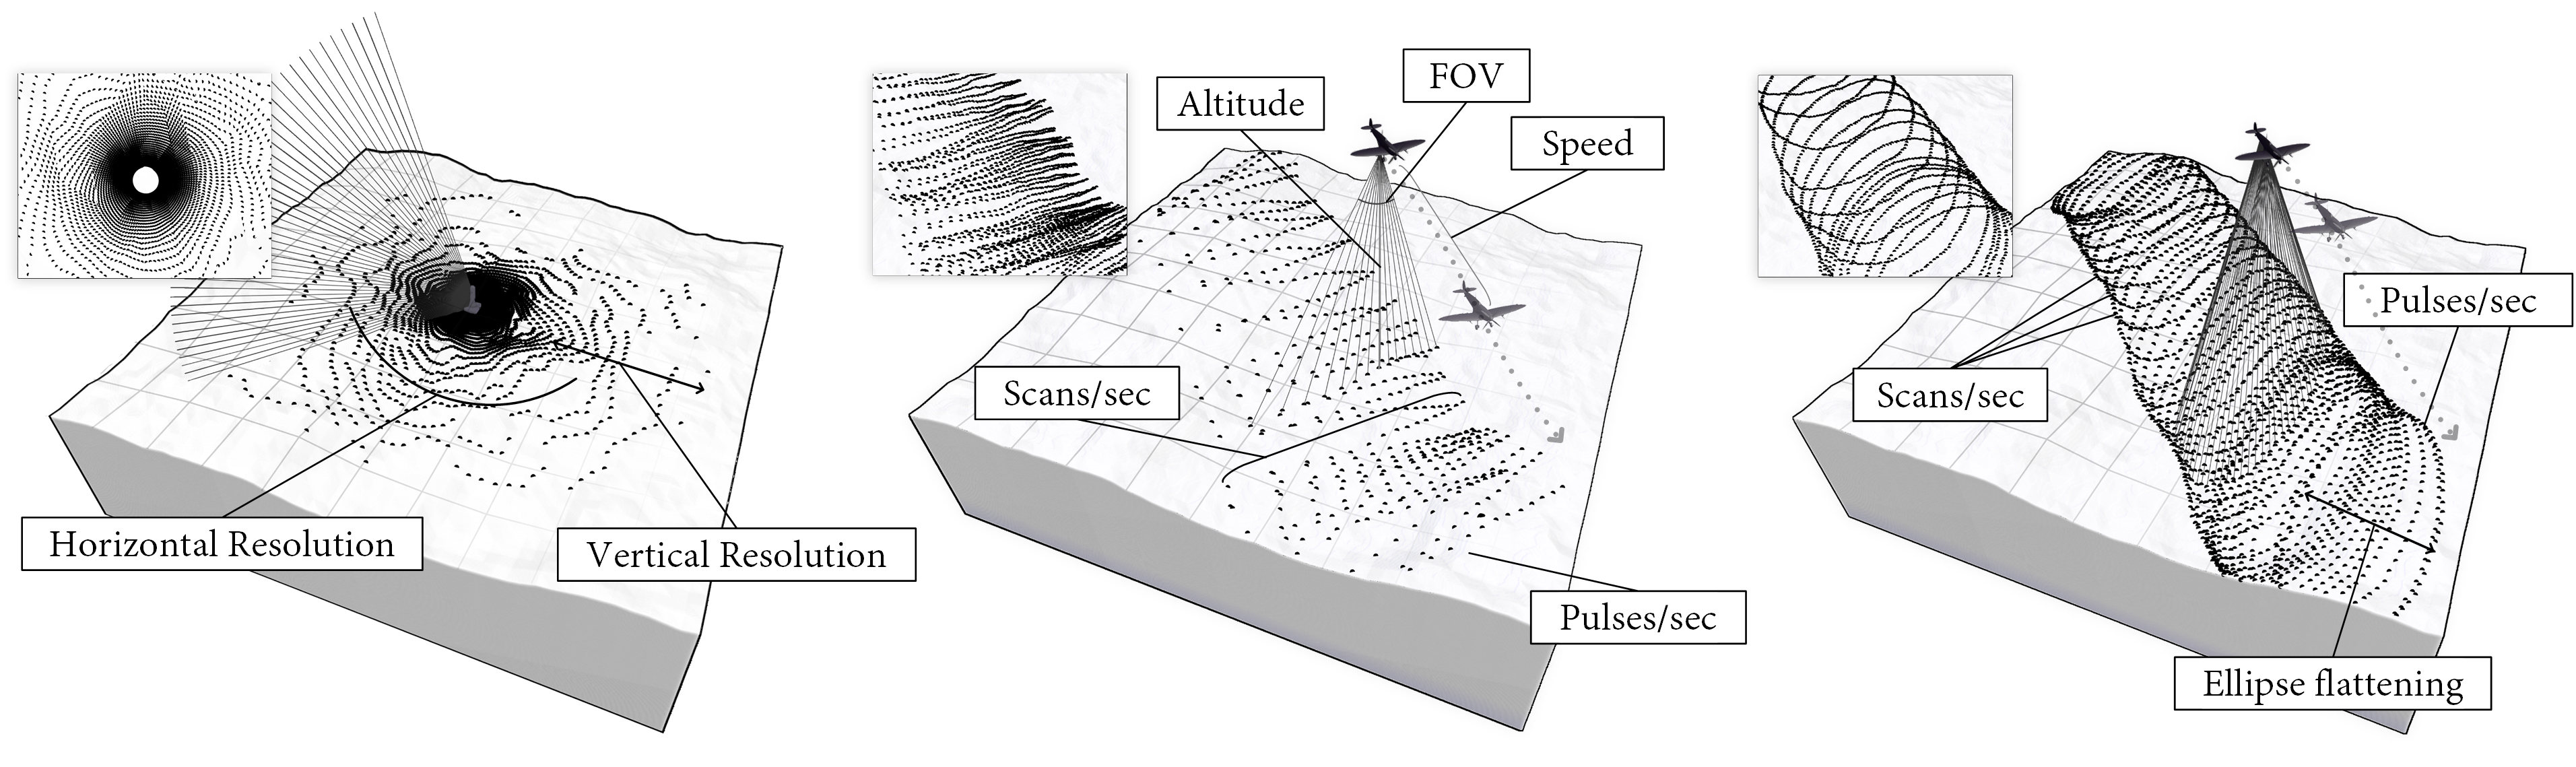
\includegraphics[width=\linewidth]{figs/fundamentals/lidar_patterns.png}
	\caption{Surveys performed with different path planning: a) the path is automatically computed according to the sensor's \acrshort{fov}, whereas in b) the path is drawn by the user, simplified using the Douglas-Peucker algorithm and subsampled using a Catmull-Rom spline. Zoomed-in images at the top-right corner show the effect of jittering. }
    \label{fig:lidar_patterns}
\end{figure*}

Most common \acrshort{lidar} operates on the 600-1000 \si{\nano\meter} spectral range for non-scientific applications; ground-based are frequently in 500-600 \si{\nano\meter}, whereas airborne systems work over 1000-1600 \si{\nano\meter}. The second is of special interest for this dissertation and thus we will stick to it. Despite being more expensive, these are also eye-safe due to working at larger wavelengths. Nevertheless, most commercial sensors operating below 1000 \si{\nano\meter} are eye-safe nowadays. Airborne \acrshort{lidar} can record several discrete measurements per emitted pulse, or record a signal sampled with a frequency determined by time interval or distance (for example, sampled every 1 \si{\nano\second} or 15 \si{\centi\meter}). The latter is known as full-waveform \acrshort{lidar} and is mainly used in forestry applications since it provides a signature that helps on estimating the density at different height levels. On the other hand, discrete-return \acrshort{lidar} has found a wider number of applications. A minimal operative \acrshort{lidar} is composed of laser and receiver units, \acrshort{gps} and \acrshort{imu} systems and control, monitoring and recording units. Hence, one of the main shortcomings of imagery is overcome by \acrshort{lidar}, as recorded 3D points are georeferenced. 
\begin{gather}
    \label{eq:lidar_distance}
    \begin{aligned}
        R &= \frac{1}{2}ct_s
    \end{aligned}
\end{gather}

Equations \ref{eq:lidar_distance} and \ref{eq:lidar_equation} may shed some light on the functioning of \acrshort{lidar} systems. First, the distance of the surface that returned the backscattered energy, $R$, is calculated according to the time delay, $t_s$, and the speed of light, $c$. Also, the acquired energy, involving both emitter and receiver, is expressed as shown in Equation \ref{eq:lidar_equation}. There are multiple formulae in the literature to represent how is \acrshort{lidar} intensity retrieved, though most are analogous \cite{hofle_correction_2007, bolkas_effect_2018, dong_lidar_2018}.
\begin{gather}
    \label{eq:lidar_equation}
    \begin{aligned}
        \sigma &= \frac{4\pi f_{r}(\vec{w})A_{t}}{\Omega}\\
        A_{t} &= \frac{\pi R^{2} \beta^{2}_{t}}{4}\\
        P_{r} &= \frac{\bar{I} D^{2}_{r} \eta_{atm} \eta_{sys} \sigma}{4 \pi R^{4}}=
        \frac{4\pi^2 \bar{I} D^{2}_{r} \eta_{atm} \eta_{sys}  f_{r}(\vec{w})}{4\Omega R^{2} \beta^{2}_{t}}
    \end{aligned}
\end{gather}
where $\bar{I}$ is the emitted energy, $D^{2}_{r}$ is the receiver diameter (\si{\meter}), $\eta_{atm}, \eta_{sys}$ are atmospheric and system transmission factors, $f_{r}(\vec{w})$ is the target reflectance, $A_{t}$ is the target area, $R$ is the distance to receiver in \si{\meter}, $\beta$ is the transmit beam width (\si{\radian}) and $\Omega$ is the scattering solid angle (\si{\steradian}). $\pi$ controls the amount of energy spreading a specific point since it spreads in every possible direction within a semisphere.

Lasers are the main unit in \acrshort{lidar} systems, and energy emitted by these can be oriented through a scanning deflector to output different scanning patterns, as depicted in Figure \ref{fig:lidar_patterns}. If the orientation of lasers varies, so does the scanning pattern. The fundamental deflections are based on polygonal mirroring, which generates parallel scan lines and swinging mirrors with zig-zag patterns, thus achieving more point density at the line boundaries. Other deflections are fibre optics, which produce a similar output to polygonal mirroring despite changing beam transmission technology, and rotating slanted mirrors that generate elliptical shapes. Finally, Risley prism scanners such as DJI Livox have a different pattern for sampling surfaces with more density and longer integration times \cite{bechtold_helios_2016, winiwarter_virtual_2022}.

Table \ref{table:lidar_devices} shows a brief list of some widespread \acrshort{lidar} sensors, both terrestrial and airborne. It provides further insight into which are the most frequent wavelengths. Among these, \acrshort{lidar} sensors operating at 532 \si{\nano\meter} are also known as bathymetric and enable capturing shallow, underwater surfaces. Thus, it is especially relevant for hydrology and coastal monitoring.

\renewcommand{\arraystretch}{1.2}
\begin{table*}
    \small
    \caption{Most common \acrshort{lidar} systems in the literature and their attributes.}
    \label{table:lidar_devices}
    \begin{tabular}{lllllll}
        \toprule
        \acrshort{lidar} system & FOV & Echoes & Maximum range & Wavelength & Channels & Points/\si{\second} \\
        \midrule
        \multicolumn{7}{c}{Velodyne}\\
        HDL-32E    & $360^{\circ}\times41.3^{\circ}$    & 2   & 80-100\si{\meter} & 903\si{\nano\meter} & 32 & 1.39M\\
        Puck/Puck LITE    & $360^{\circ}\times30^{\circ}$    & 2   & 100\si{\meter} & 903\si{\nano\meter} & 16 & 600K\\
        Puck Hi-RES    & $360^{\circ}\times20^{\circ}$    & 2   & 100\si{\meter} & 903\si{\nano\meter} & 16 & 600K\\
        ULTRA Puck    & $360^{\circ}\times40^{\circ}$    & 2   & 100\si{\meter} & 903\si{\nano\meter} & 32 & 1.2M\\
        Alpha Prime    & $360^{\circ}\times40^{\circ}$    & 2   & 250\si{\meter} & 903\si{\nano\meter} & 128 & 4.8M\\
        \cmidrule{1-7}
        \multicolumn{7}{c}{Valeo}\\
        SCALA Gen 2    & $133^{\circ}\times10^{\circ}$    & 3   & 200\si{\meter} & 905\si{\nano\meter} & 16 & 25\si{\hertz}\\
        \cmidrule{1-7}
        \multicolumn{7}{c}{SICK}\\
        MRS1104C-111011    & $275^{\circ}\times7.5^{\circ}$    & 3   & 64\si{\meter} & 850\si{\nano\meter} & 32 & 165K\\
        \cmidrule{1-7}
        \multicolumn{7}{c}{Phoenix Systems}\\
        SCOUT-M2X   & $360^{\circ}\times40.3^{\circ}$    & 3  & 300\si{\meter} & 905\si{\nano\meter} & 32 & 640K\\
        SCOUT-32   & $360^{\circ}\times40^{\circ}$    & 2  & 220\si{\meter} & 905\si{\nano\meter} & 32 & 600K\\
        HydroRANGER   & $40^{\circ}$ VFOV  & 15  & 75\si{\meter} & 532\si{\nano\meter} & - & 200K\\
        RANGER-LR LITE   & $360^{\circ}$ HFOV  & 5  & 1000\si{\meter} & 1550\si{\nano\meter} & - & 1.5M\\
        \bottomrule
    \end{tabular}
\end{table*}
\renewcommand{\arraystretch}{1}

\subsection{Principles of physical measurement}

\acrshort{rs} covers a wide range of spectral wavelengths depicted in images that show the emitted and reflected radiation from the Earth's surfaces, including matter such as atmospheric particles and bare soil. A huge number of conditions and parameters are involved in the observed radiation, whose explanation would cover dozens of pages, if not a book. Hence, only a few remarks will be done here. 

A key ingredient in the understanding of the scene is the detailed specification of the appearance of materials regardless of light and the influence of other matter. Energy, as captured in nature, does not depict the underlying appearance of materials but the appearance when some specific circumstances are met. Therefore, measurements ought to be processed to make them independent from environmental and light conditions as well as surrounding surfaces. Not only it helps in the classification of materials present in the scene, given some reference spectral signatures, but also enables simulating lighting as occurs in real-world scenarios. For the latter, surfaces are assigned a spectral appearance that will not be rendered as so and thus will undergo changes as light and other matter interfere. 

\begin{figure}[bht]
	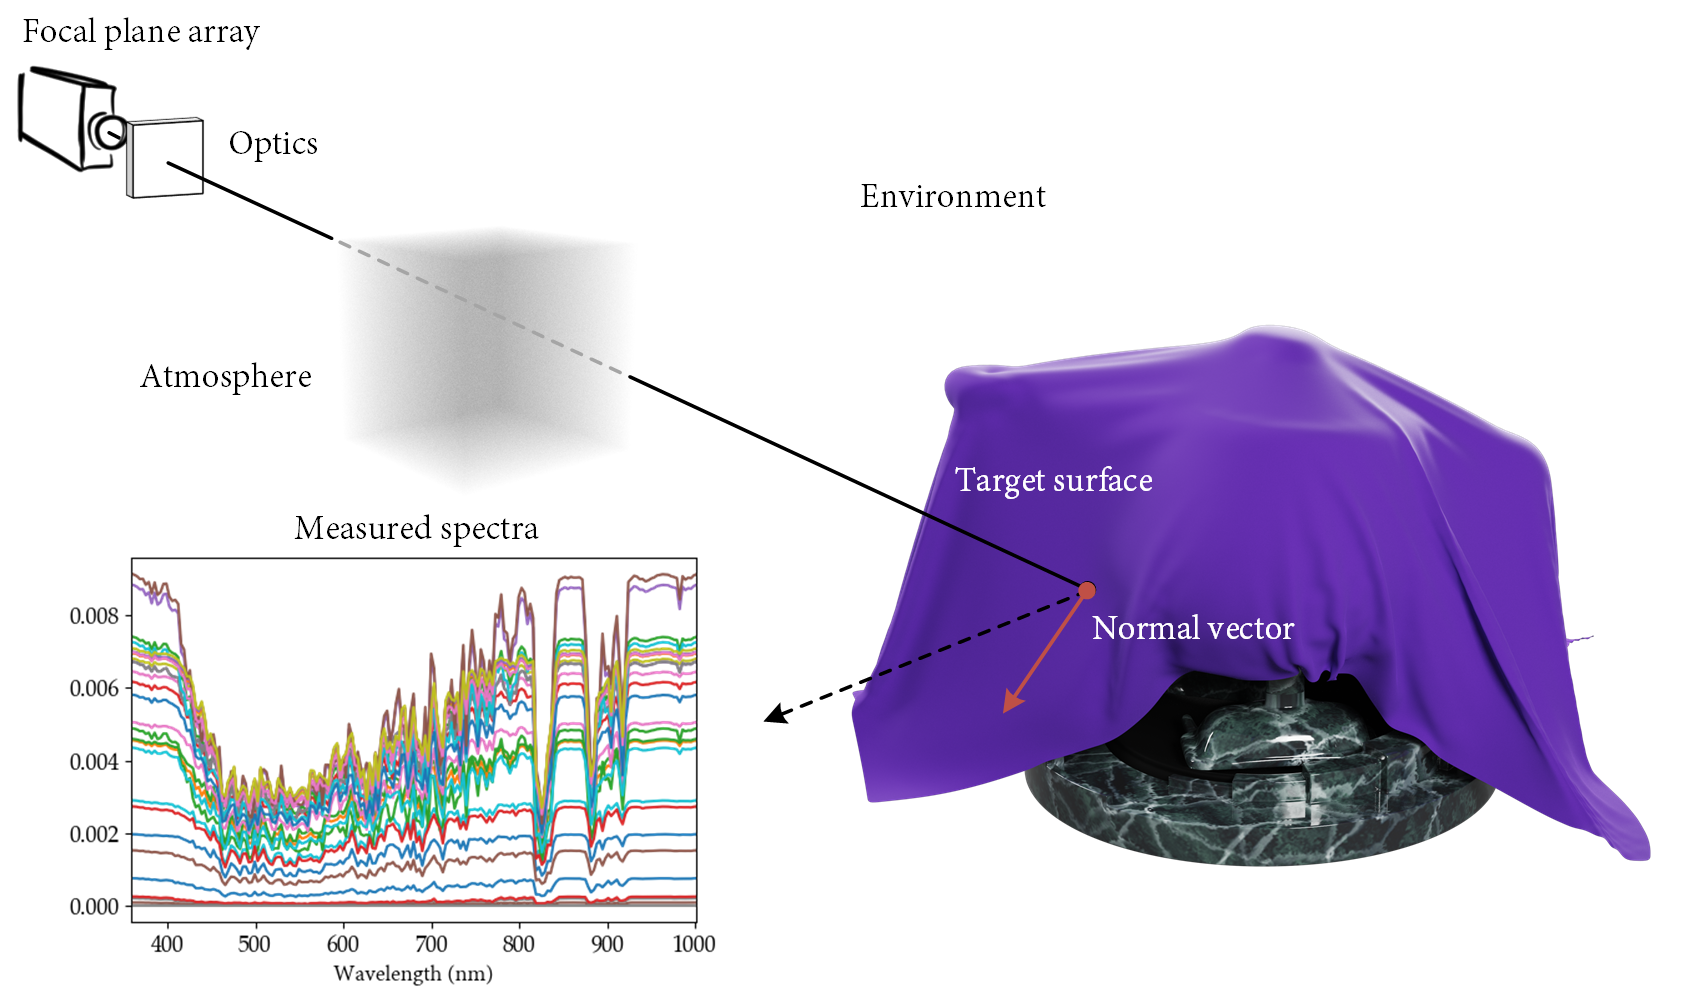
\includegraphics[width=\linewidth]{figs/fundamentals/physic_principles.png}
	\caption{Parameters that intervene in the measurement of radiance with a passive sensing tool. }
    \label{fig:physic_principles}
\end{figure}

Vollmer and Mollmann \cite{vollmer_infrared_2017} provided an exhaustive list of parameters conditioning the material emissivity, regardless of surrounding objects. Materials are the most differentiating feature, naïvely split into metal and nonmetal, where the latter are frequently returning higher emissivity. Also, the roughness level affects the outcome considerably; polished surfaces have lower emissivity and the contrary happens for rough surfaces. Further insight into energy dispersion helps to understand that it does not propagate over every direction of a semisphere with the same strength. Unlike blackbodies, which behave as perfect isotropic emitters, materials vary the emitted radiation conditioned to the outgoing direction. A key factor in this regard is the normal vector of the surface: the smaller the angle between the camera view direction and the normal vector, the higher the observed emissivity. However, this does not hold up for every material since conductors show the opposite behaviour. Similarly, the physical behaviour of light transport, including reflections, leads to increasing the emissivity for grooved surfaces as a consequence of rebounds. As will be observed throughout this dissertation, the spectral signature of materials is not constant, and therefore, some intervals are preferred over others in the seek of capturing a high emissivity from the target surfaces. For example, the \acrshort{nir} interval comprises the peak emissivity of vegetation. Finally, surface temperature also leads to slight emissivity changes.

\begin{marginfigure}[-5cm]
	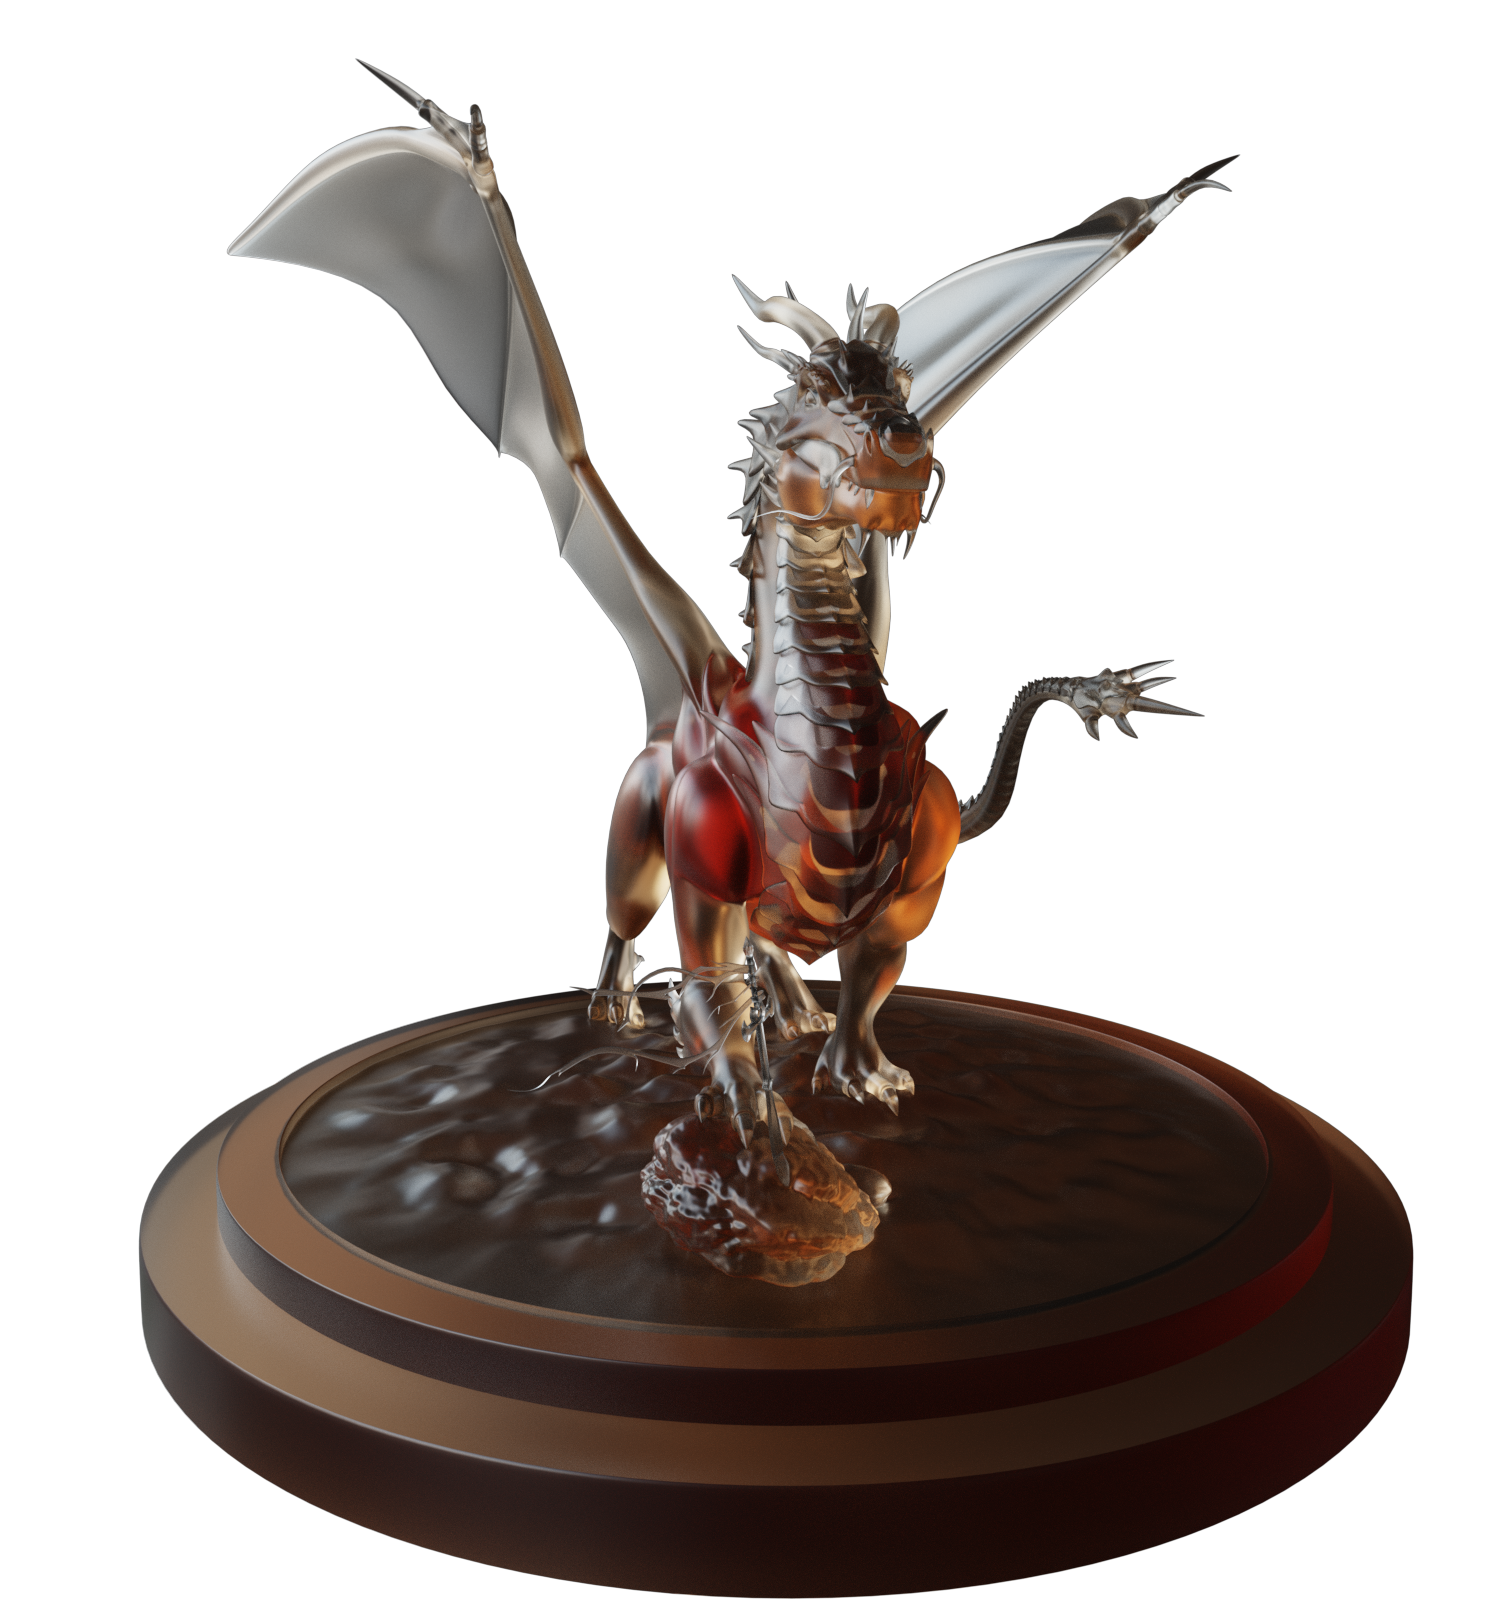
\includegraphics{figs/fundamentals/bssdf_2.png}
	\caption{Subsurface scattering simulated over a triangle mesh.}
	\label{fig:bssdf}
\end{marginfigure}
Radiometric measurements are layered data that can be carved to find the surfaces' spectral signatures. However, the carving process relies on corrections that are simple approximations considering a few of the mentioned factors rather than the overwhelming amount of uncontrolled attributes that can be found in nature. Otherwise, measurements can be performed with controlled surface features and lighting to provide databases of a wide range of materials \cite{dupuy_adaptive_2018}. Furthermore, databases on surface appearance comprise a number of discrete spectral signatures for each material, as these are typically parameterized by the input vector, $\omega_i$, and the output direction where radiance spreads, $\omega_o$ (Figure \ref{fig:brdf_wi_wo}). Otherwise, these vectors can be notated as local cartesian coordinates, half-angle difference parametrization and spherical coordinates, which are also very frequent \cite{montes_soldado_overview_2012}. The latter are expressed through four angles, $\varphi_i = \atan(y_i / x_i)$, $\varphi_o = \atan(y_o / x_o)$, $\theta_i = \acos(z_i)$ and $\theta_o = \acos(z_o)$. These functions, provisionally expressed as $f(\omega_i, \omega_i)$, parameterized with $\omega_i$, $\omega_o$, or their equivalent spherical coordinates, represent what was coined as Bidirectional Reflectance Distribution Functions (\acrshort{brdf}), or yet more intricate, Bidirectional Scatter Distribution Functions (\acrshort{bsdf}) and Bidirectional Scattering Surface Distribution Functions (\acrshort{bssdf}). Both \acrshort{bsdf} and \acrshort{bssdf} are aimed at simulating the indirect light transport from surrounding surfaces as well as their own surfaces. \acrshort{bssdf} are particularly hard to calculate as the entering and exit points vary, i.e., surfaces are not opaque (see Figure \ref{fig:bssdf}); instead, light travels through matter to provide a transparent-like, yet opaque, appearance. From now on, we will only refer to \acrshort{brdf} as the two last functions are beyond the scope of this dissertation.
\begin{marginfigure}[-1.2cm]
	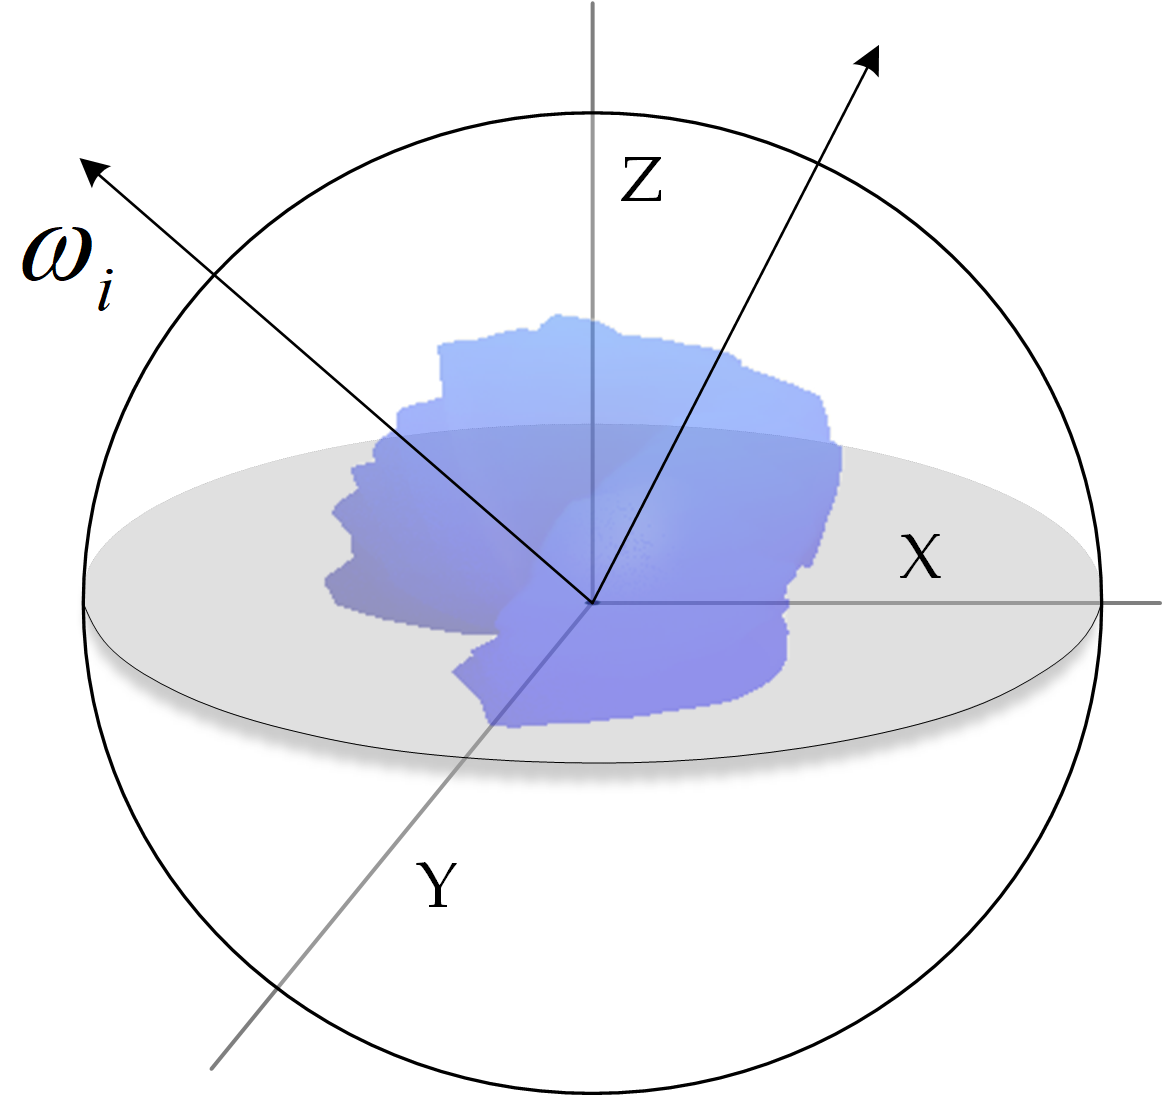
\includegraphics{figs/fundamentals/brdf_wi_wo.png}
	\caption{Parameterization of the \acrshort{brdf} response.}
	\label{fig:brdf_wi_wo}
\end{marginfigure}

In the last years, hyperspectral data acquisition has significantly increased, benefiting from the use of more cost-effective sensors and versatile platforms. On the one hand, traditional systems, which are deployed in the laboratory, are currently more efficient and capable of getting accurate spectral measurements of isotropic and anisotropic materials. These are gaining in accuracy, efficiency, and ease of use. At the laboratory level, the most accurate and well-known technique for collecting the optical features and \acrshort{brdf} of any real-world material is the use of a goniophotometer \cite{riviere_multispectral_2012}. Different variants of this configuration have been developed either to obtain better results in anisotropic materials, to take into account refraction phenomena or even to obtain normal maps, and any other characteristic that helps in synthetic modelling \cite{tunwattanapong_acquiring_2013, chen_reflectance_2014}. 

The first databases only included anisotropic materials that captured red, green and blue spectral response as a dense set of measurements \cite{matusik_data-driven_2003}, instead of analytical functions. Thus, discretized representations are more likely to be parameterized to build larger, yet realistic, \acrshort{brdf} datasets \cite{serrano_intuitive_2016}. More recently, the provided wavelengths have been extended to the whole spectra available for a motorized goniophotometer, thus allowing to extend render engines beyond the visible spectra \cite{dupuy_adaptive_2018}. As a result, \acrshort{brdf} are not solely parameterized through two spatial vectors, but also with a radiometric value. Hence, $f$ is now expressed as $f(\omega_i, \omega_o, \lambda)$, with $\lambda$ being the target wavelength. Accordingly, coarse radiometric resolution can be simulated as $\int_{\lambda_i}^{\lambda_j} f(\omega_i, \omega_o, \lambda) \hspace{1mm} d\lambda$. 

These advances lead us toward the generation of real-world material databases, which are notably used for rendering photorealistic scenes, virtual interior design in architecture, the game industry, etc. These applications can be enhanced by the increasing availability of real-world scenarios, which can be efficiently reconstructed using versatile platforms. However, building material databases is time-consuming, prohibitive when it comes to acquisition devices and requires considering a list of laboratory constraints. 

Due to the large measurement time, \acrshort{uas} flights carrying a hyperspectral sensor have been proposed for the collection of material \acrshort{brdf}. These come at expense of noisier data that must be corrected afterwards. In addition, a single or a few flights yield very incomplete spatial response due to the low variety of $\omega_o$ measurements \cite{jurado_efficient_2022}. There have been studies on atmospheric corrections for \acrshort{uas} flights, which involve correlating the at-sensor radiance to the \acrshort{hdrf} measured in the laboratory beforehand. Grayscale palettes in Lambertian materials can be used for this purpose  \cite{lucieer_hyperuasimaging_2014}. While physically-based methods have also been explored, they tend to be more time-consuming. In addition, public repositories such as the Aviris data portal (California Institute of Technology) \cite{california_institute_of_technology_aviris_nodate} offer atmospherically corrected datasets. Other widespread hyperspectral processing software, such as ENVI and Headwall SpectralView, include semi-automatic correction algorithms \cite{queally_flexbrdf_2022, jia_kernel-driven_2020, sagan_data-driven_2022}.

The lack of computational power and real-world material samples led to approximate realistic shading with analytical functions. These are easier to solve and integrate into script-based routines such as vertex and fragment shaders. They intend to emulate the appearance of real-world materials; however, continuous functions are smoothed-out versions that include errors as a consequence of fitting real data. Furthermore, fitting functions in non-linear optimizations is expensive to compute, whereas analytical functions have a low memory footprint and enable simulating a wide range of materials (with more or less precision). Hence, this \acrshort{brdf} representation was widely adopted until recently. 

\begin{marginfigure}[3cm]
	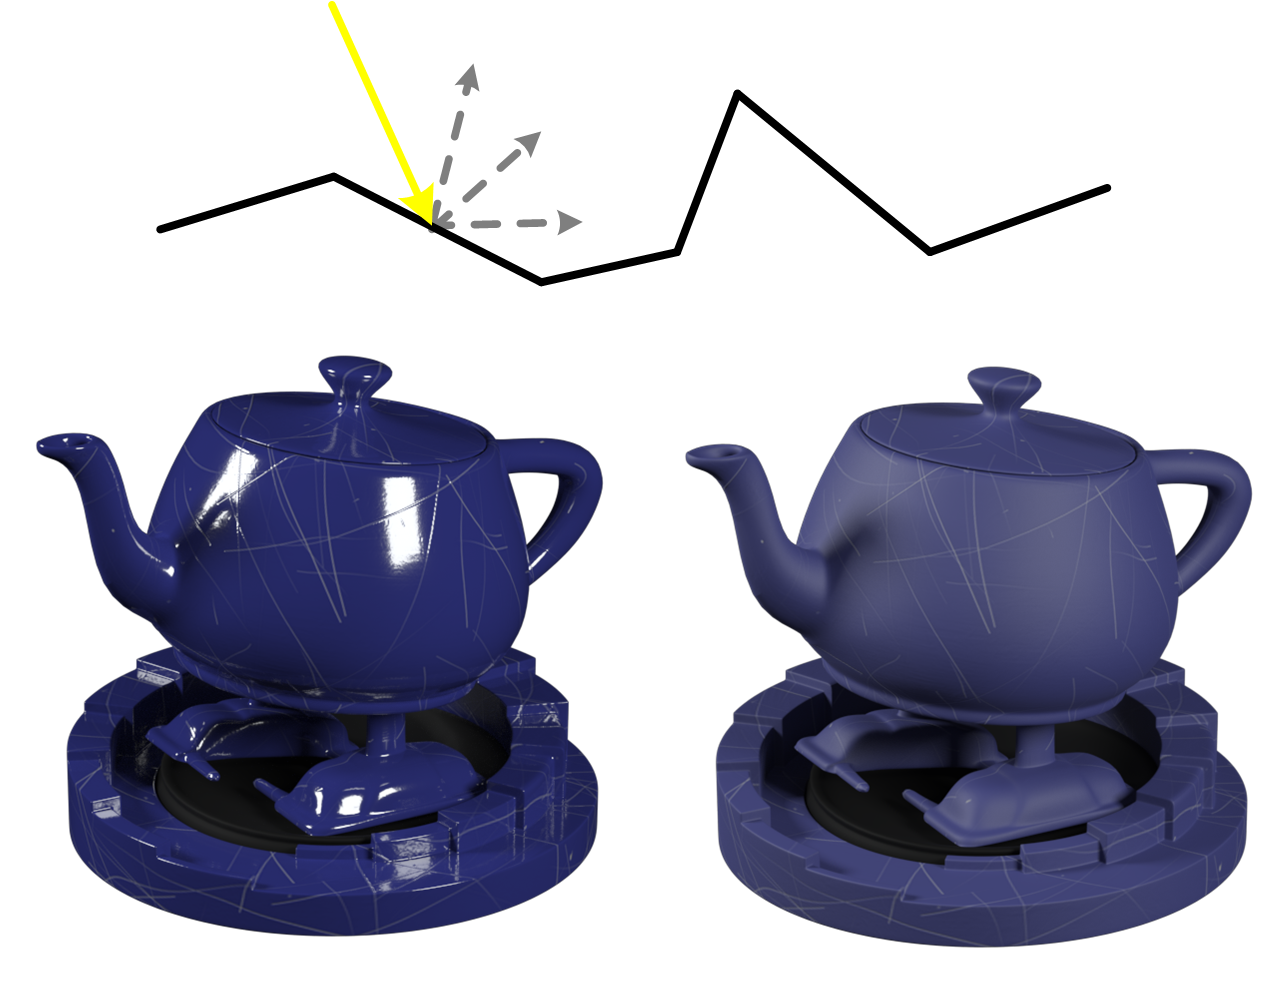
\includegraphics{figs/fundamentals/microfacets.png}
	\caption{Insight into micro facets of a surface. The striking energy reflects into the semisphere formed on the basis of the normal vector. Below, the same object is rendered as a polished and rough surface. Therefore, the second present microfacets that lead to a wider energy scattering.}
	\label{fig:microfacets}
\end{marginfigure}
Analytical \acrshort{brdf}s have a large taxonomy if we attend to the kind of material and the criteria under which these were modelled. Although most of them aim to simulate a specific appearance (metal, wood, mats, polished surfaces, the Moon, etc.), materials are at least organized into isotropic and anisotropic materials. The firsts are invariant to rotations of the surface around $n$, whereas the second changes its reflection around $n$, emulating materials such as hair or brushed metal \cite{guarnera_brdf_2016}. On the other hand, \acrshort{brdf}s are categorized as phenomenological or empirical, physically-based or theoretical and data-driven. Phenomelogical functions are computationally convenient methods for estimating the reflectance appearance of some materials, whereas theoretical make use of some attributes that intervene in physically-based shading. For instance, Phong was one of the first phenomenological models that were widely adopted with the advent of programmable pipelines. It is simply parameterized by the surface normal, $n$, the lighting vector from a single source, $l$, the view direction, $v$, and the reflection, $r$, computed according to the Fresnel law. On the other hand, Cook-Torrance is one, if not the most, representative theoretical \acrshort{brdf} as it pays attention to micro-facets, distinguished metal and dielectrics and uses the halfway vector, $h$, to compute the specular lobe. For novel \acrshort{cg} programmers, this is frequently introduced as the foundational core of Physically-Based Rendering (\acrshort{pbr}) for shader-based frameworks such as \acrshort{opengl} (Open Graphics Library). For further insight into analytical \acrshort{brdf}s, we refer the reader to the explanations of these from a theoretical point of view \cite{guarnera_brdf_2016, soldado_overview_2012}. Note that radiance spreads over a semi-sphere, and therefore, most of these functions include $\pi$ in the denominator, whereas the numerator is scaled by the $\cos$ function parameterized by $\omega_i$, $\omega_o$ and $n$. However, traditional \acrshort{cg} applications avoid downscaling the computed intensity by $\pi$ since it darkens the rendered scene and they do not intend to behave as physically-based engines. A simple demonstration of Minnaert \acrshort{brdf} is shown in Code \ref{code:analyticalbrdf}, firstly implemented to render intensity in a semi-sphere, whereas the second block is rather aimed at shading a polygonal mesh.

\vspace{3mm}

\lstinputlisting[language=c++, caption={Minnaert \acrshort{brdf} implementation for a 1) reflectance visualization tool using a semi-sphere and 2) a rendering application.}, label=code:analyticalbrdf]{code/minnaert.brdf}

\begin{figure}[ht]
	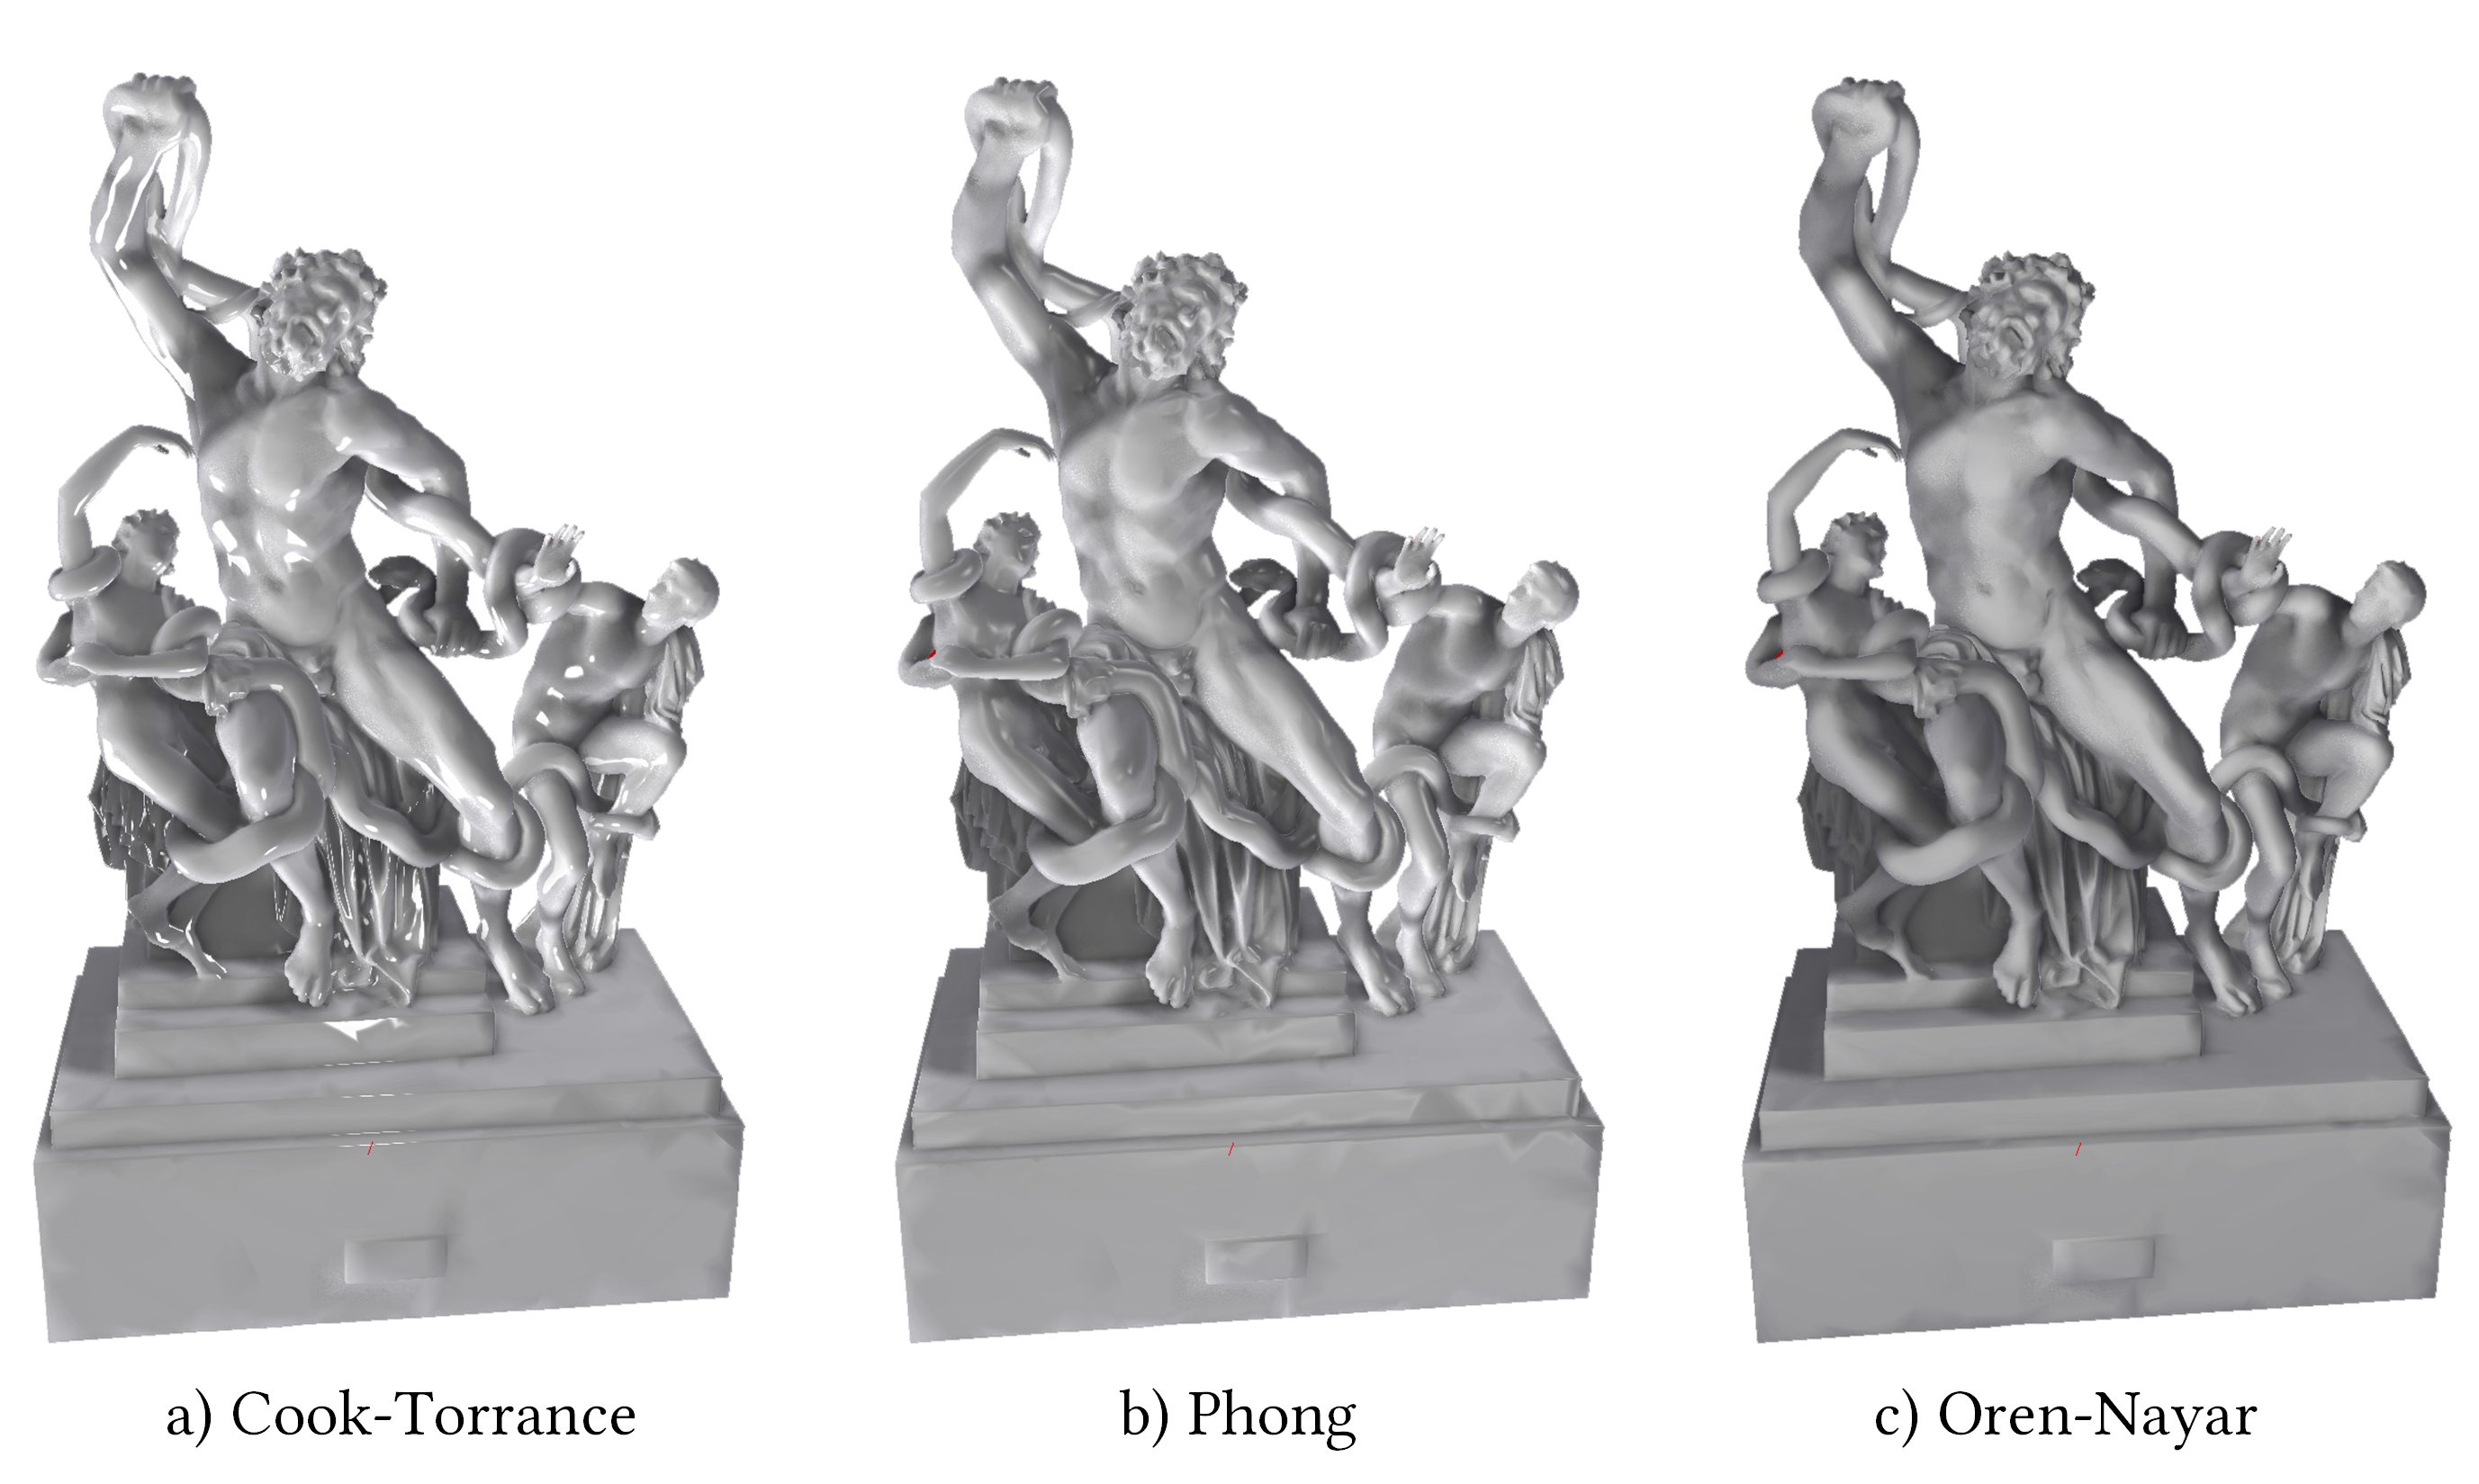
\includegraphics[width=\textwidth]{figs/fundamentals/analytical_brdf.png}
	\caption{Comparison of analytical \acrshort{brdf}s: a) Cook-Torrance ($f_0 \gets 1$, $\alpha \gets 0.077$), b) Phong ($ns \gets 32$) and c) Oren-Nayar ($\alpha \gets 0.75$). }
    \label{fig:analytical_brdf}
\end{figure}

% \begin{figure*}[ht]
%     \imageannotated{figs/fundamentals/room_rt.png}{Hello world}{0}{-2.6}{white}
% 	\caption{Comparison of analytical BRDFS: a)  }
%     \label{fig:hello}
% \end{figure*}

\section{Data types, processing and indexing}

Once the imaging devices and the interaction of light and matter have been revised, the results provided by most \acrshort{rs} tools are explained, including the main challenges that we must address if these will be the focus of our work. Then, other traditional processing algorithms which are later used are explained. These algorithms are either based on the image space or operate with 3D point clouds.

\subsection{Results from Remote Sensing}

\subsubsection{Image: vector and raster}
\label{sec:rs_data_formats}

The concept of images seems very straightforward, though the focus of this section is on the adjective preceding the image term. Besides human impression of someone or something, images are defined as "any picture, especially one formed by a mirror or a lens" by Cambridge Dictionary \cite{cambridge_english_dictionary_cambridge_2023} and "a picture of somebody/something seen in a mirror, through a camera, or on a television, computer, phone, etc." in Oxford Dictionary \cite{oxford_university_press_oxford_2023}. As a mathematical concept, an image is "a point set or set formed by mapping from another point or set", thus requiring \textbf{at least} two point sets to form an image. The subdivision of images over $\mathcal{X}$ and $\mathcal{Y}$ axes yields what is known as a pixel: the images' primitive. Despite being unique pieces of information, these are highly correlated among them and thus influenced by surrounding pixels. The significance of this conclusion is later exposed in this document to discriminate the plant variety captured in a pixel.
\marginnote[-1cm]{At least two point sets are required to form an image, though the most frequent images in the wild have three channels (visible imaging) and thus require more than two sets. For \acrshort{rs}, images with up to hundreds of channels are required for precise monitoring and data mining.}

Hence, images are discrete representations where each pixel shows the average captured radiance. However, these values are not the originally measured radiance. Instead, an Analog-to-Digital (A-to-D) conversion transforms the electrical signal into values known as Digital Numbers (\acrshort{dn}). These are typically integer values that fall in the interval $2^x$, with $x \gets 8$ being the most frequent radiometric depth \cite{navulur_multispectral_2006}, though float-point values can also be found for file formats storing uncompressed representations, e.g., \acrshort{tiff}. The radiometric resolution is especially relevant for scientific purposes where A-to-D leads to a loss of precision. Other not-that-frequent file formats store embedded \acrshort{dn}s in the image metadata, such as radiometric \acrshort{jpeg}, thus allowing us to obtain the temperature afterwards. Despite images being here referred to results acquired by sensors, the term "image" covers any pictorial representation, even generated on computers. Unlike sensing tools, computers have the advantage of working with digital data whose geometrical shapes can be defined by means of step-wise and continuous functions. As a result, the internal encoding of images does not always fits into the previous mathematical definition. The images that are not defined as a set of pixels, but rather as a set of geometrical shapes, are known as vector images instead of raster images. While vector data have no limitations on the resolution and present a lower memory footprint, raster data is easier to analyze and include in Geographic Information Systems (\acrshort{gis}) together with other layers acquired with similar spatial resolution \cite{lillesand_remote_2015}. Still, vector data is especially relevant for visualization, including \acrshort{gis} aimed at mapping Earth's cities and infrastructure (see Figure \ref{fig:raster_gis}). A comparison of raster and vector data is depicted in Figure \ref{fig:raster_vectorial}.
\begin{marginfigure}[-6.8cm]
	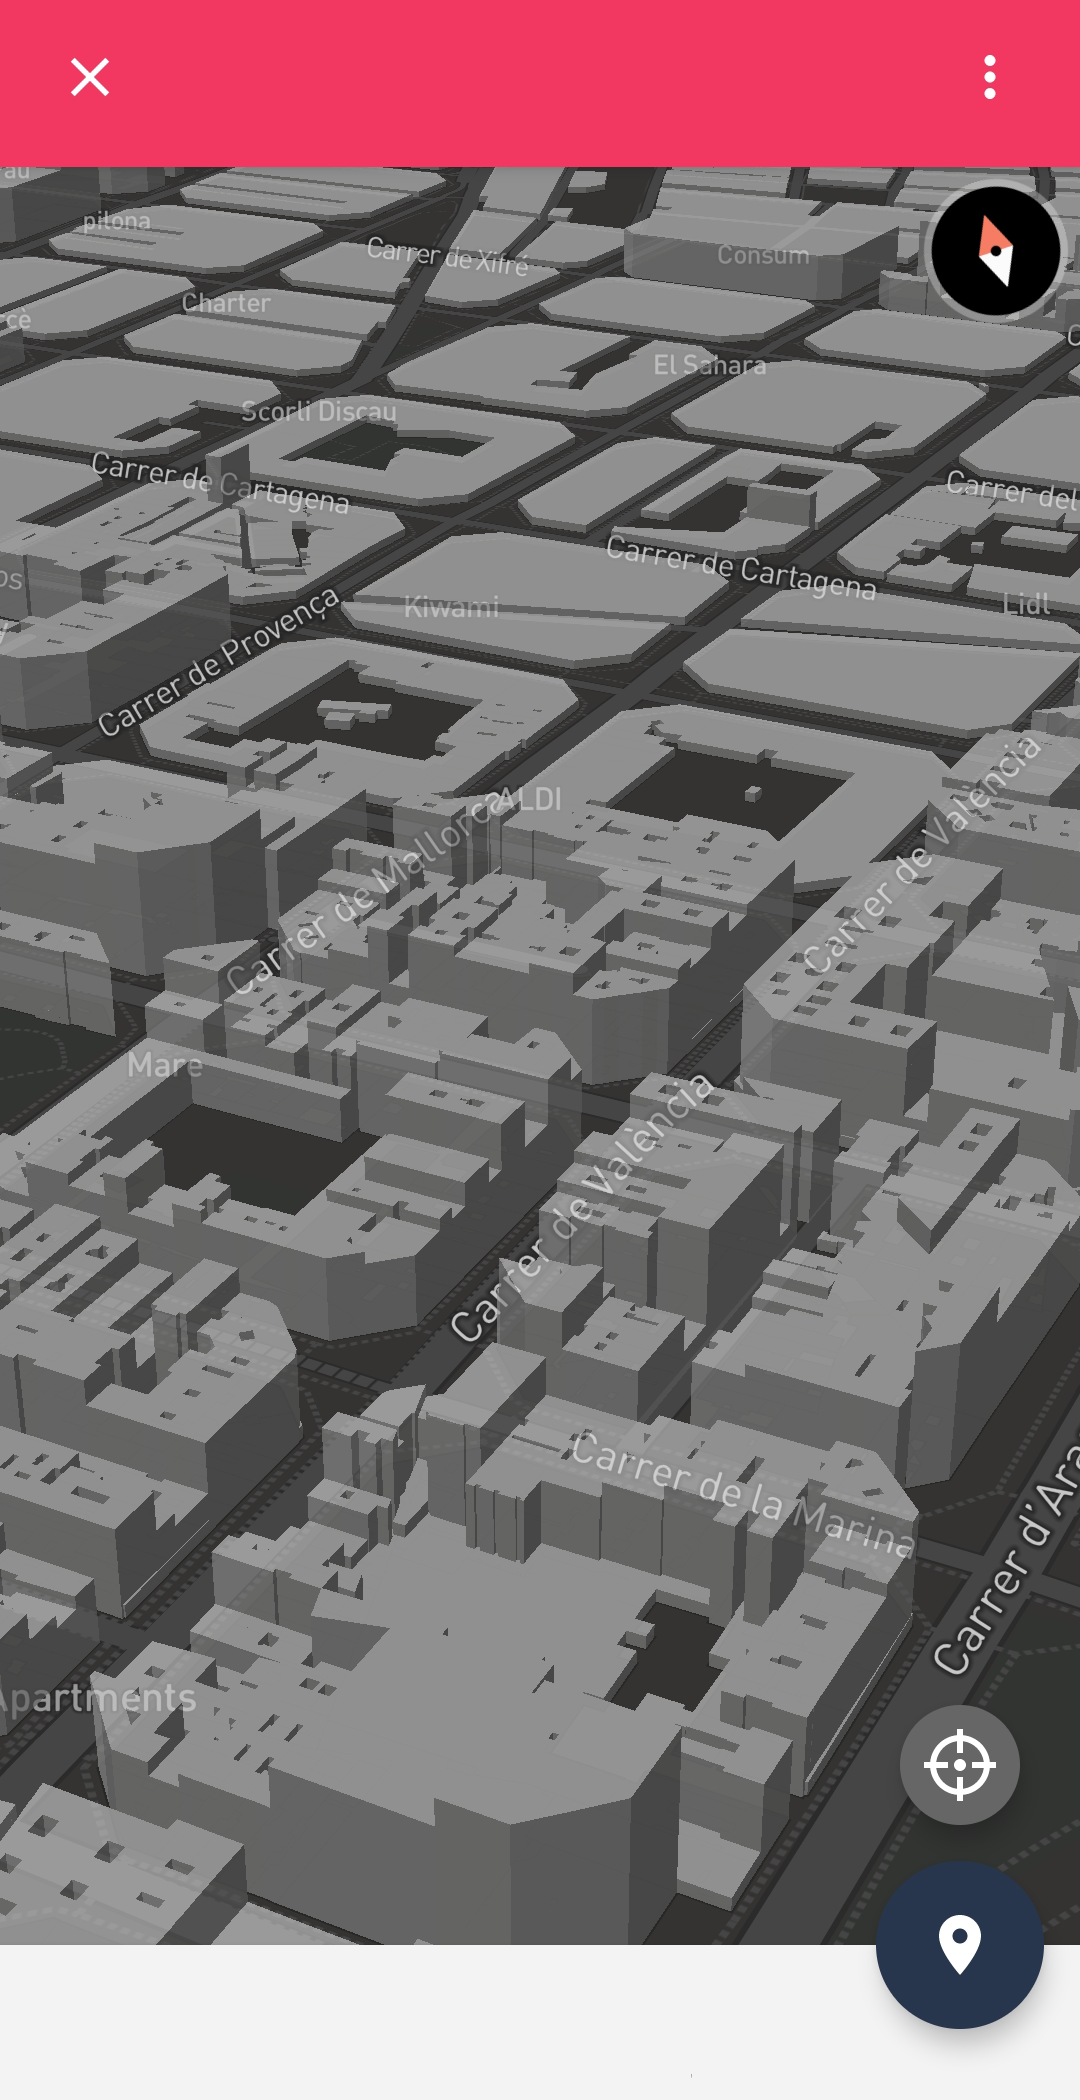
\includegraphics{figs/fundamentals/raster_gis.png}
	\caption{Vector data in a geographic information system within an Android application.}
	\label{fig:raster_gis}
\end{marginfigure}

\begin{figure}[ht]
	\includegraphics{figs/fundamentals/raster_vectorial.png}
	\caption{Comparison of a) raster and b) vector representation of Vila Real District in Portugal.  }
    \label{fig:raster_vectorial}
\end{figure}

The spatial resolution of images refers to the number of pixels represented in $\mathcal{X}$ and $\mathcal{Y}$ axes. However, it can be further stressed to introduce the amount of space in \si{\meter^2} represented in a pixel. Indeed, the latter concept is more frequent in \acrshort{rs}. It is typically derived from the image dimensions and the distance covered in $\mathcal{X}$ and $\mathcal{Y}$.

The most widespread impression of images is colour-space examples. However, there exists a considerable imagery taxonomy organized from the number of bands ($\mathcal{Z}$) and the information that is encoded in each of them. The most revised kinds of imagery are visible (colour-space), thermographic, multispectral and hyperspectral. The sensors that capture this information are coined with the same name. In this regard, Figure \ref{fig:sensor_literature} shows the percentage of research devoted to each one of the mentioned tools in the last few years. Minority tools such as \acrshort{rgb}-D, with D standing for depth, are omitted in this figure. Previous sections have delved into each one of these sensors, and their results are explained in this section. The Scopus searches were the following: $(\epsilon \cdot (\mathtt{rgb} \lor \mathtt{visible}) \lor \epsilon \cdot (\mathtt{thermal} \lor \mathtt{thermography}) \lor \epsilon \cdot \mathtt{multispectral} \lor \epsilon \cdot \mathtt{hyperspectral}) \land ((\mathtt{remote} \land \mathtt{sensing}) \lor \mathtt{uas} \lor \mathtt{uav}), \hspace{1mm} \epsilon \in \{0, 1\}$, where $\epsilon$ refers to the selection of one of the sensor keywords. 

\begin{figure}[ht]
	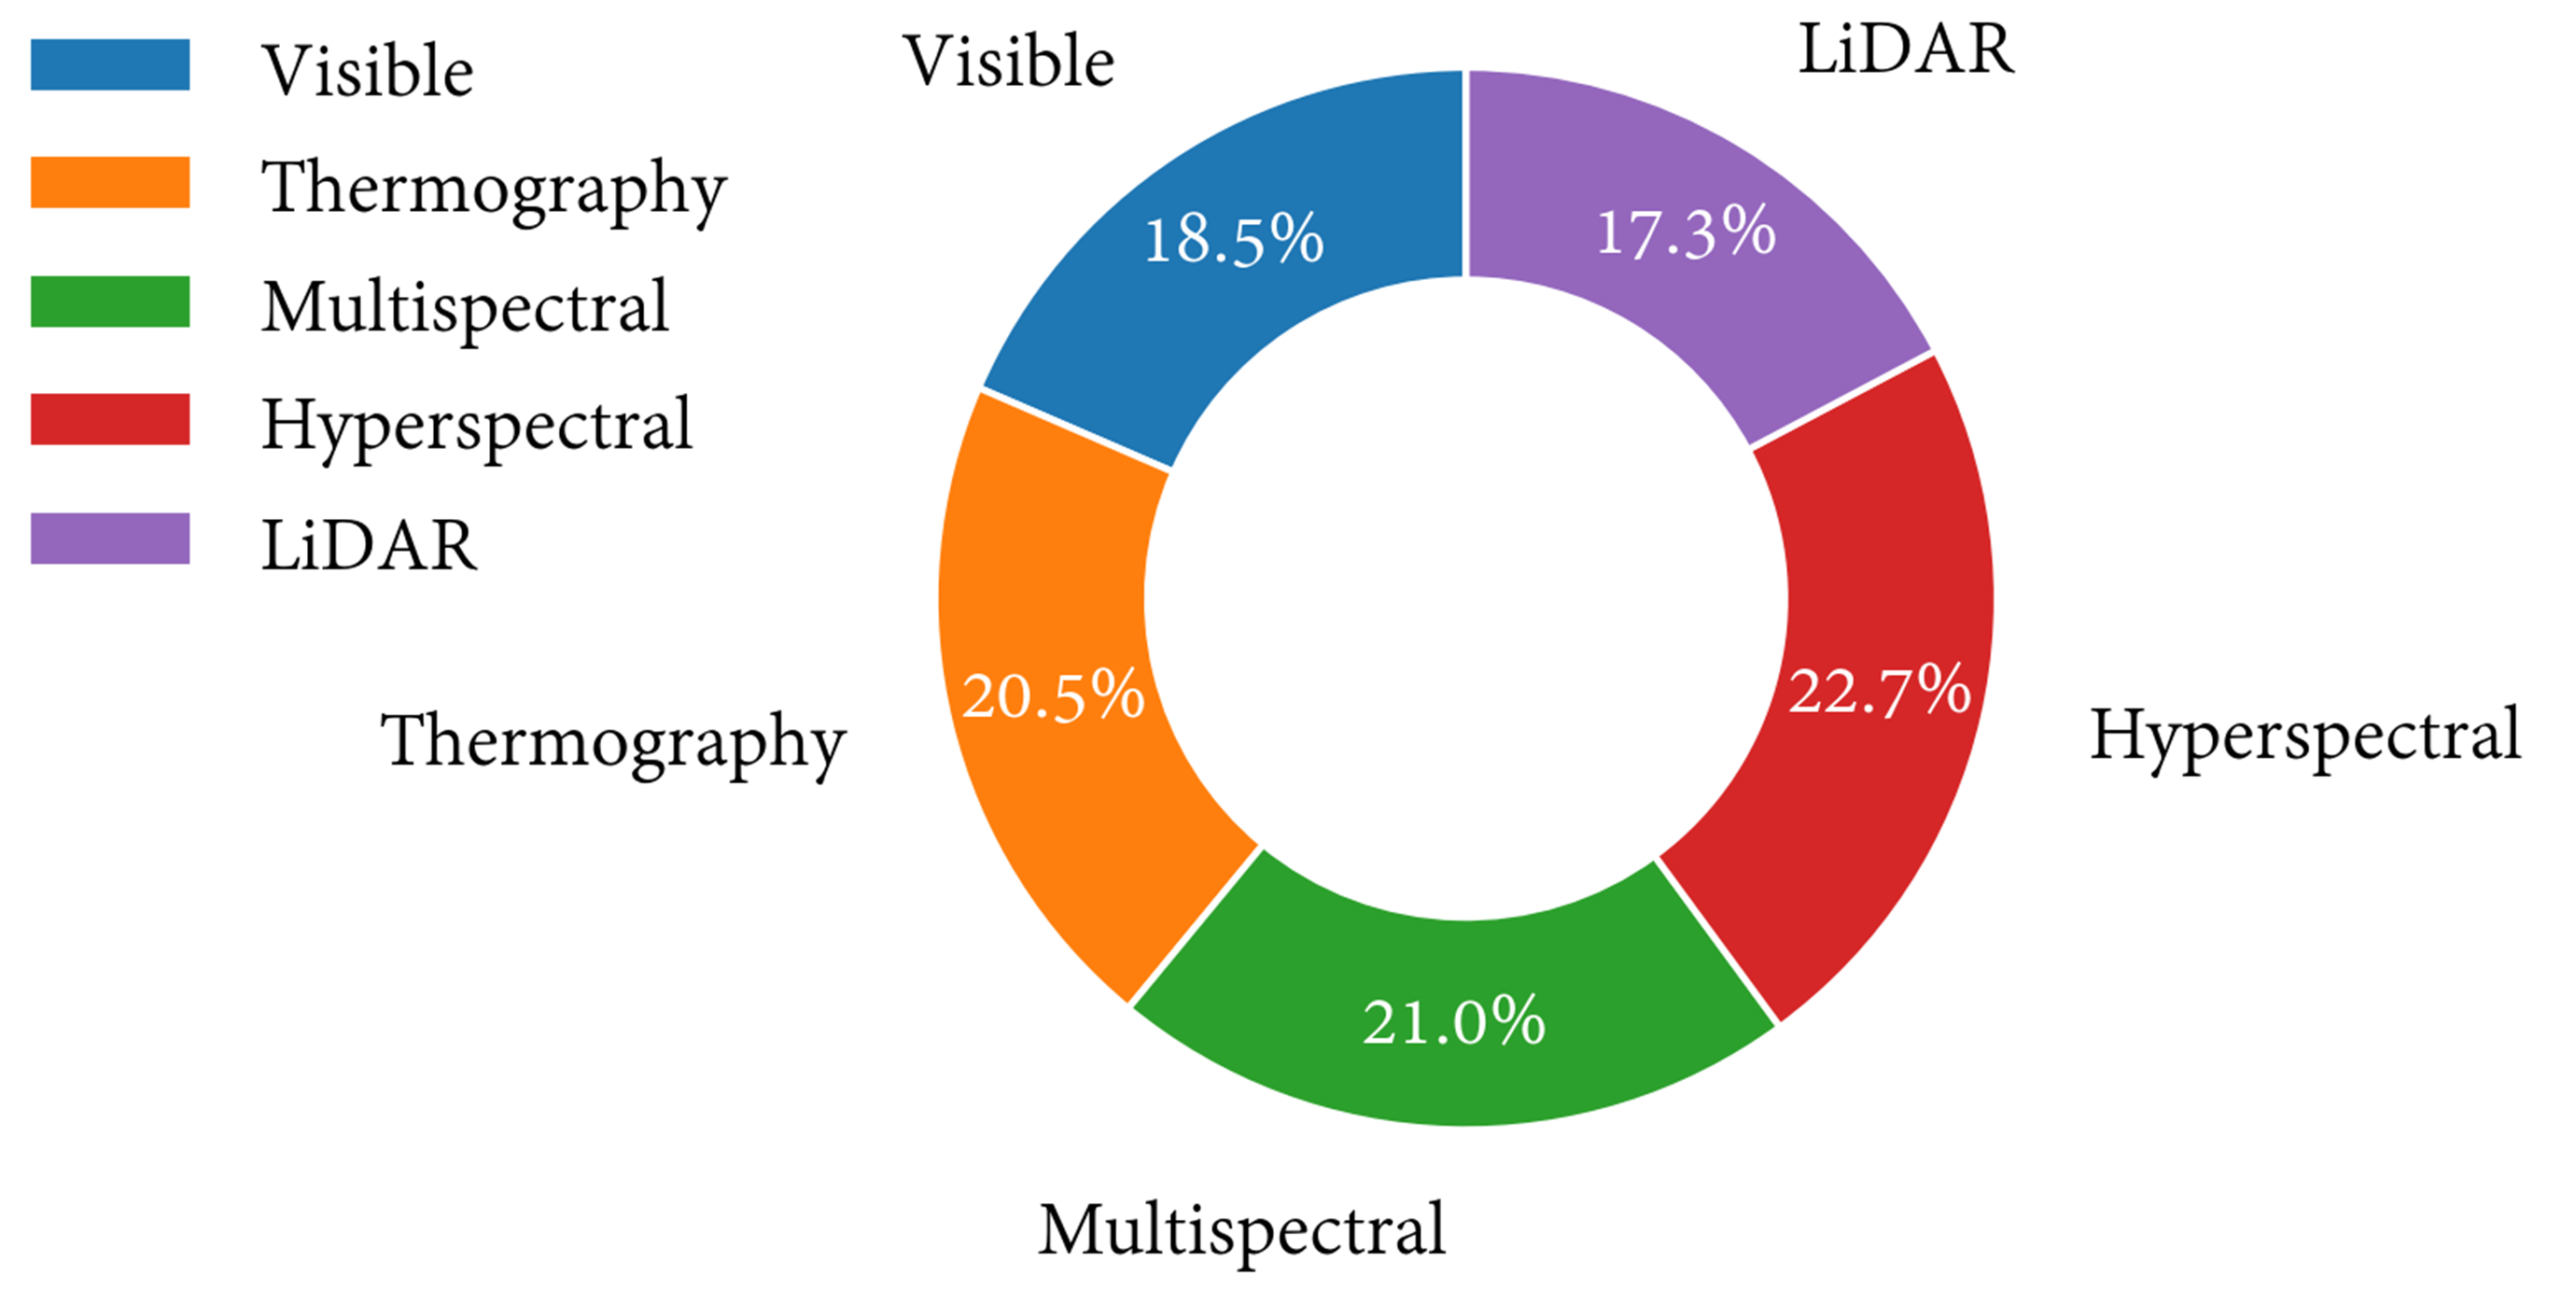
\includegraphics[width=.9\textwidth]{figs/fundamentals/literature_sensors.png}
	\caption{Number of manuscripts related to different sensors.  }
    \label{fig:sensor_literature}
\end{figure}

\subsubsection{Point clouds}

Point clouds are collections of points with no connectivity, which are typically extracted from laser scanners and photogrammetry. There exists an enormous number of hardware and software solutions measuring real-world geometry at a constant pace, including the so-called digital twins. Although images carry relevant features and lead to meaningful conclusions, these are not linked to geometry. Three-dimensional representation of real-world scenarios has enjoyed a great interest to improve visualization and interpretation of the surveyed areas and phenomena. Therefore, 3D point clouds derived from imagery can be generated, if not directly acquired with passive sensing, to facilitate the view of buildings, surfaces and any other area of interest. In contrast to 3D meshes, they enable a simpler, denser and close-to-reality representation \cite{cao_3d_2019}. Besides the positioning, points can carry further information, including colour, reflectance, intensity, normal vector and classification label, among others. Additionally, all these values can be replicated at different timestamps throughout the time scale. Reviewing the scientific literature, it can be concluded that this problem is similar to that posed in the technique called projective texture mapping \cite{debevec_efficient_1998, heckbert_survey_1986}. Initially, the aim was to have additional effects on the realistic image synthesis field of research, to cast shadows or render translucent objects \cite{dachsbacher_translucent_2003}.

The staggering pace of information acquisition and requirements concerning the level of detail of point clouds lead to massive 4D data, thus hardening the efficient storage, transmission and visualization. Yet, they are widely used in fields as disparate as autonomous driving systems, virtual and augmented reality, biomedical applications and precision agriculture. Geometric features provide further data that helps with the recognition and classification of objects, even for human operators. For instance, previous work \cite{barros_multispectral_2022, kerkech_vine_2020, de_castro_3-d_2018} have shown that elevation data significantly improves the classification accuracy on the segmentation of plots, with elevation being a derived product of photogrammetry and passive sensing. However, huge point clouds consisting of billions, even trillions of points, require up-to-date techniques that benefit from nowadays hardware, capable of massively working in parallel. The current state-of-the-art studies have extensively worked on the compression of point clouds, to save storage and reduce bit rate transmission, as well as on the efficient visualization of massive point clouds \cite{schutz_gpu-accelerated_2023, van_oosterom_organizing_2022}. 

Other operators such as the estimation of normal vectors will be following explored as it concerns a later chapter. However, this is simply a minimal part of research on point clouds, since the uncertainty from photogrammetry and laser point clouds must be individually addressed for each application. Part of this enormous amount of work comprises the classification, segmentation and identification of tree skeletons \cite{cardenas_reconstruction_2022} on point clouds. 

\subsection{Data processing}

\subsubsection{Compression}

The huge amount of point cloud data represents a challenge both for storage and transmission. Furthermore, the following massively parallel operations are performed on \acrshort{gpu} hardware with limited memory capacity. Although this drawback has been mitigated in the most recent \acrshort{gpu}s (NVIDIA GeForce 40 series at the moment this dissertation is being written), these operations ought to work over commodity hardware. The most recent releases have a memory size ranging from 8 GB (GeForce RTX 3050) to 24 GB (GeForce RTX 3090, GeForce RTX 3090 Ti \cite{nvidia_nvidia_nodate-2} and GeForce RTX 4090 \cite{nvidia_nvidia_nodate-1}), whereas laptop models have typically their memory size reduced to half of these. Other high-performance \acrshort{gpu}s focused on research, for example, NVIDIA A6000 \cite{nvidia_nvidia_nodate}, scale up to 48 GB and enable higher capacity using a bridge called NVIDIA NVLink. However, these high-performance products are not widespread, and most computers work using commodity hardware. Accordingly, GeForce Series 10 and 20 are less prohibitive, easier to acquire under stock shortage and more frequent to find in laptops not designed for high-performance tasks. The memory size of these devices is below 12 GB for Series 20 and 8 GB for Series 10. 

Furthermore, there exist frameworks for \acrshort{gpu} visualization and computing that severely clamps the maximum buffer size. For instance, \acrshort{opengl} has been the standard platform for visualization for decades. Version 4.3 introduced what is known as computer shaders, i.e., scripts solving small \acrshort{gpu} tasks that can be massively parallelized. One would expect to be able to reserve buffers with a maximum size bounded by the \acrshort{gpu}'s memory capacity; however, this limit can be queried in \acrshort{opengl}, with the \scriptsize \verb|GL_MAX_SHADER_STORAGE_BLOCK_SIZE| \normalsize keyword, returning 2,048 MB both for an NVIDIA GTX 1070 (8 GB VRAM) and an NVIDIA RTX A6000 (48 GB VRAM).

Hence, massive point clouds require at some point to be compressed, mainly in transmission and visualization applications. This research field has been coined as \acrshort{pcc}, Point Cloud Compression, distinguishing lossy and lossless methods. Similar to the computer science field, \acrshort{pcc} has transitioned from traditional techniques \cite{bui_comparative_2021}, based on encoding using data structures (regular grids, octrees, kd-trees, etc. \cite{cao_3d_2019}) to Deep Learning, where the encoding is automatically learned by convolutional autoencoders (\acrshort{cnn-ae}). The latter are more likely to lose data to some degree unless the compressed data is discrete \cite{que_voxelcontext-net_2021}, such as octree nodes. 

Very few compression methods offer low-computational complexity for real-time transmission \cite{cao_3d_2019} and reconstruction (decoding), while others do not support the compression of colour information. However, \acrshort{rs} point clouds can carry large amounts of information for every point; from \acrshort{lidar} points whose attributes follow the \acrshort{las} file standard to hyperspectral points storing spectral signatures with hundreds of measurements. Rather than exploiting the point cloud's entropy in the spatial and temporal dimensions, Graciano et al. \cite{graciano_quadstack_2021} proposed to compress layered datasets taking advantage of data redundancy. Although it was proposed to volumetric data from geology, biology or medicine fields, redundancy of sensor measurements can also be exploited for rendering. The algorithm is composed of three main steps: 1) stack redundant values on the $\textit{z}$ dimension to form the stack-based representation (\acrshort{sbr}) from the initial heightfields, 2) group stacks with the same stack content (G-stacks) and 3) organize these into a quad-tree. Spatial redundancy is not as relevant for sensor data since it captures a wide variety of materials, whereas spectral compression is feasible at expense of downscaling the radiometric resolution. 

\subsubsection{Visualization}

\begin{marginfigure}[.0cm]
	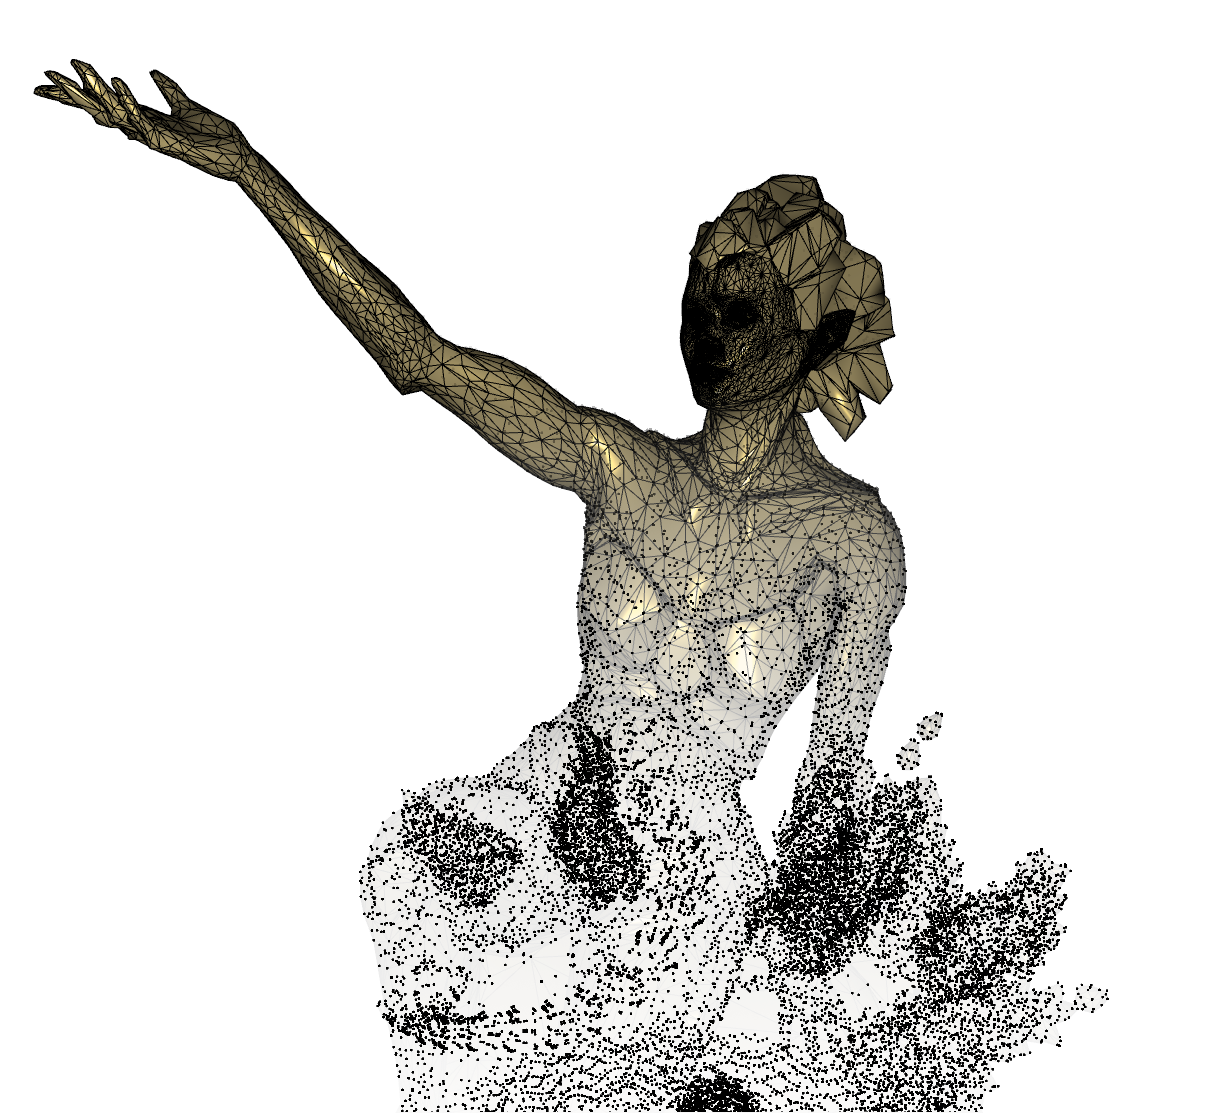
\includegraphics{figs/fundamentals/triangle_mesh_point_cloud.png}
	\caption{Transition from triangle mesh to point cloud representation, from top to bottom, with the second solely showing the triangles' vertices.}
	\label{fig:triangle_mesh_pc_comparison}
\end{marginfigure}
Unlike triangle meshes intending to emulate continuous surfaces with underlying discrete polygons, point clouds are discrete representations. Therefore, visualizing the latter is harder for scarce products with low point density (see Figure \ref{fig:triangle_mesh_pc_comparison}). This hardens the detection of features and extraction of valuable information by human operators. Computationally, it implies increasing the neighbourhood distance from which features are extracted or simply obtaining imprecise results due to the lack of data. The traditional rendering pipeline neither helps to accelerate the visualization of massive point clouds. It is designed for polygonal meshes that require 1) processing vertices, 2) including additional geometry, 3) discarding non-visible geometry, 4) rasterizing polygons, and 5) colouring polygon fragments \cite{akenine-moller_real-time_2018}.

The current state-of-the-art of massive point cloud rendering has evolved along with the impressive work of Schütz and Wimmer \cite{schutz_rendering_2019, schutz_rendering_2021}. The aim of their work was not only to speed up the visualization of billions of points but also to improve the rendered image. \acrshort{opengl}'s compute shaders were used to generate the images in the \acrshort{gpu} and recently introduced NVIDIA extensions helped to further optimize it. An alternative rendering procedure is built over \acrshort{opengl} to omit the stages 2), 3) and 4) of the traditional pipeline. In this work, vertices were massively projected into an image that is later rendered as a texture. However, the order in which points were projected showed to have a big impact on the performance. Points were transformed into Morton codes of 30 bits, 10 for every dimension, and sorted according to them. Then, globally sorted points were shuffled into small batch groups, whose size is determined by Graphic Processing Clusters (\acrshort{gpc}s). Rather than distributing the work linearly, the \acrshort{gpu} organizes it into 2D patches assigned to \acrshort{gpc}s. Thus, global sorting helps in grouping framebuffer updates, but it is suboptimal due to workload unbalancing. Spatially close \acrshort{gpc}s in charge of visible points at a timestamp $t$ are assigned a heavy workload, while others remain idle. The random shuffling of globally sorted points using small batches was proved to slightly enhance the rendering performance.

\begin{figure}[ht]
	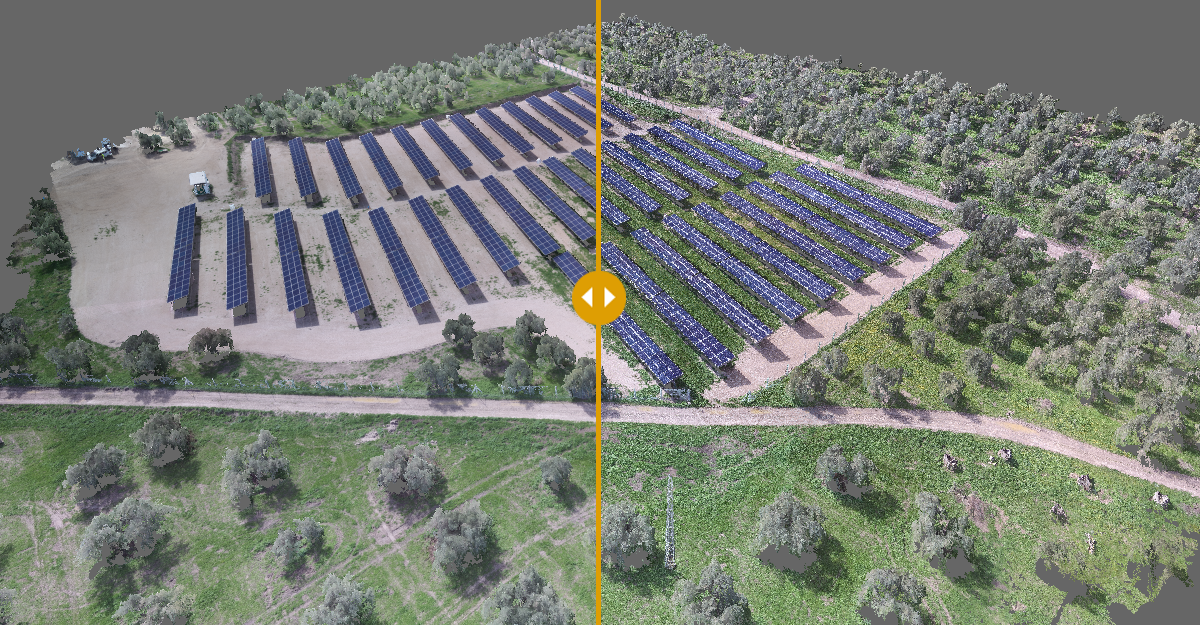
\includegraphics[width=\textwidth]{figs/fundamentals/hqs_comparison.png}
	\caption{On the left part, colouring using a mixed representation of surrounding points and on the right side, using a sole point colour for each pixel. This image was obtained using the procedure described by Schütz and Wimmer \cite{schutz_rendering_2021}. }
    \label{fig:hqs_pc_rendering}
\end{figure}

\begin{kaobox}[frametitle=Compute shader core proposed by Schütz and Wimmer]
The projection approach from Schütz and Wimmer \cite{schutz_rendering_2021} uses modern \acrshort{opengl} extensions following this pipeline:
\begin{itemize}
    \item The depth buffer is firstly computed, with the depth being encoded along with the point index (64 bits). The atomic minimum operators help to select the point with the minimum depth. However, this approach leads to a noisy-like rendering for sparse point clouds. Instead, the depth of a pixel takes into account several points; data is exchanged within thread groups whose points fall in the same pixel using \verb|shuffleNV| and \verb|ballotThreadNV| operators. Then, \verb|shuffleXorNV| computes the minimum depth within a pixel neighbourhood.
    \item Colours are iteratively accumulated: the limited capacity of SSBOs may require that multiple point cloud subdivisions aggregate data. Accumulations can be implemented using atomic operators, whereas (red, green) and (blue, alpha ($\alpha$)) channels are encoded in two different buffers with values of 64 bits. Hence, the alpha channel is also used for accounting for the number of visible points at each pixel.
    \item Aggregated colours are finally transformed by averaging the mean value for each channel. Pixels with $\alpha \gets 0$ are coloured with the background tone. 
\end{itemize}
\end{kaobox}

Lately, optimizations of point cloud renderings have focused on the \acrshort{lod} and organization into Layered Point Clouds (\acrshort{lpc}). A key in the construction of these data structures is that they ought to be view-dependent to enable adjusting the \acrshort{lod} based on the camera position and direction. \cite{schutz_gpu-accelerated_2023} proposed to index point clouds with octrees whose inner nodes are voxelized, whereas leaf nodes lead to the point primitives. Ogayar et al. \cite{ogayar-anguita_nested_2023} managed to create an adaptive hierarchical structure that coupled different data structures at different levels. It was shown to retrieve larger amounts of points with higher average and peak throughput. Previously, Schütz et al. \cite{schutz_software_2022} sorted points with their Morton codes, split them into batches and built a hierarchical data structure using these batches as leaf nodes. Visualization of \acrshort{lod}s varies according to the camera, and therefore, patches of different point densities could be rendered for distant objects. If the underlying discrete levels of a \acrshort{lod}-based data structure are visible, they are referred to as rendering artefacts. Van Oosterom et al. \cite{van_oosterom_organizing_2022} proposed to organize point clouds into a Space Filling Curve (\acrshort{sfc}) and compute the continuous \acrshort{lod} of every point, thus enabling gradual changes in the point density. 

Noise in point cloud visualization was also mitigated by Schütz et al. \cite{schutz_rendering_2019, schutz_rendering_2021} using modern \acrshort{opengl} extensions. Individual \acrshort{gpu} threads are grouped in subgroups, also known as warps, of size 32 in NVIDIA microarchitectures, that can communicate efficiently and exchange results. For a globally sorted point cloud, warps work over spatially close points that can aggregate colour data. Hence, this approach leads to a High-Quality Shading (\acrshort{hqs}) variant \cite{schutz_rendering_2021} that provides a more continuous shading (see Figure \ref{fig:hqs_pc_rendering}). This also opens the possibility of filling holes derived from lower point density rather than reconstruction failures. 

\subsubsection{Occlusion detection}

The projection of additional sources of information over point clouds is trivial once camera poses are estimated. For each viewpoint, the camera matrix enables the projection of 3D points into the image plane. However, projections do not separate background and foreground surfaces; although a point may be theoretically visible from a camera, it could be covered by another surface in the real scenario. The chances are that points are visible in more than a single viewpoint, and therefore, erroneous assignments of information may be partially masked by other correct measurements. However, this approach is not precise for colouring point clouds and occlusion must be detected to tackle this.    

\begin{marginfigure}[-3cm]
	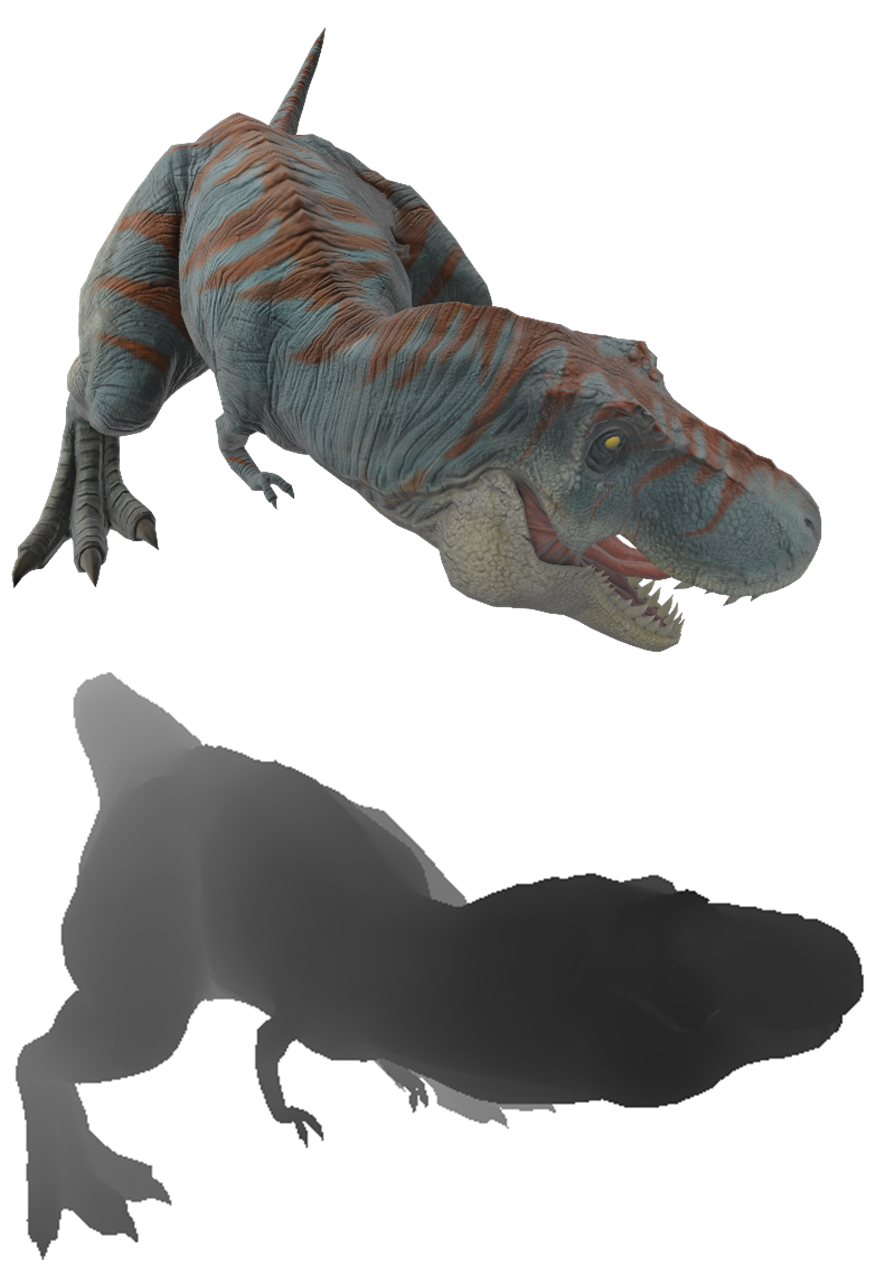
\includegraphics{figs/fundamentals/z-buffer.png}
	\caption{Shading of a 3D model along with the depth captured in a $z$-buffer.}
	\label{fig:z-buffer_opengl}
\end{marginfigure}
The most straightforward way to detect occlusion is to use what is called $z$-buffers in rendering: images that store for each pixel the minimum depth at which geometry was projected. It has been traditionally used for shadowing and discarding non-visible geometry for optimizing the rendering \cite{akenine-moller_real-time_2018, white_cascaded_2021}. Similarly, it enables recording the nearest visible point at every image's pixel. It does not require indexing points into a data structure, though they are of great help to narrow the subset of points to be projected into a single viewpoint. Determining the nearest depth is trivial in the \acrshort{gpu}, as most \acrshort{gpgpu} frameworks provide atomic operations. Despite these being supposedly slower operations, they compete well against other approaches in terms of memory consumption and efficiency. Jurado et al. \cite{jurado_out--core_2022} proposed to build out-of-core occlusion-aware multispectral point clouds in Compute Unified Device Architecture (\acrshort{cuda}). Asynchronous data loading and computation were applied to complete $z$-buffers for hundreds of images and point clouds of up to 1,084M points. Instead of using $z$-buffers, Jo et al. \cite{jo_dense_2021} computed the point and camera distance to solely project information from the closest viewpoint. This approach leads to errors if the point remains occluded from the closest one, though it can work over very dense and uniform image datasets. Not to mention this colour assignment is more prone to noise, while aggregations mitigate it. 

\begin{figure}[ht]
	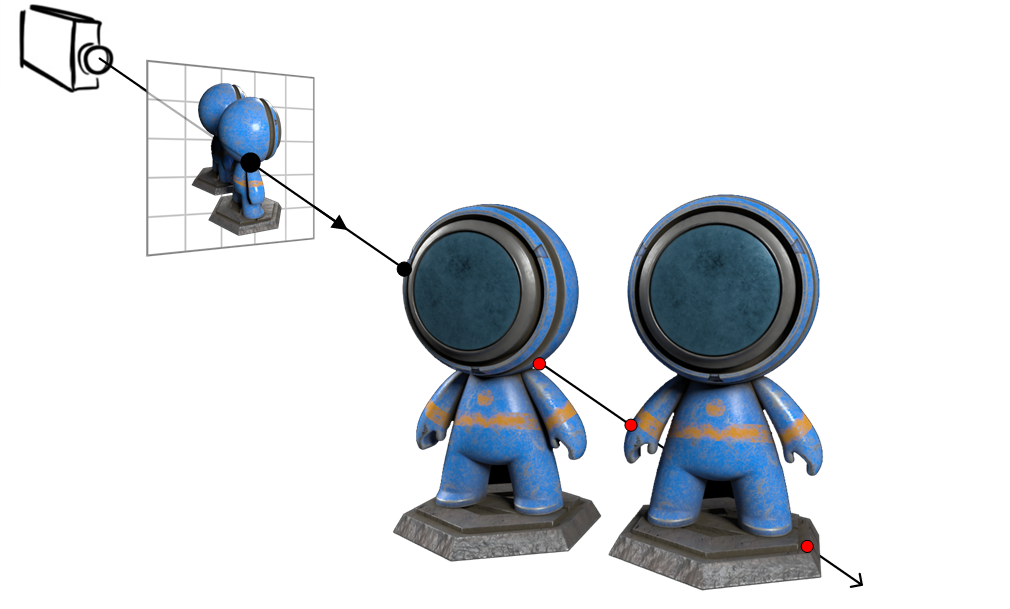
\includegraphics[width=\textwidth]{figs/fundamentals/occlusion.png}
	\caption{Occlusion of left figure over the right one on a projection made from the left part of the scene. }
    \label{fig:occlusion_concept}
\end{figure}

An alternative to $z$-buffers is to estimate the underlying polygon mesh of point clouds. In this regard, occlusion can be detected by constructing a small triangle mesh from points surrounding the main one \cite{jurado_multispectral_2020}. The point neighbourhood was sought using $k$-nearest neighbours (\acrshort{knn}). Although this method may achieve good results over planar surfaces, polygonal meshes are harder to reconstruct in other scenarios, for example, forestry with dense and incomplete vegetation. Other studies benefit from additional sources of information to detect occlusion, such as the semantic segmentation of point clouds \cite{schneider_fusing_2010}. 

\subsubsection{Photogrammetry}

\begin{marginfigure}[2.0cm]
	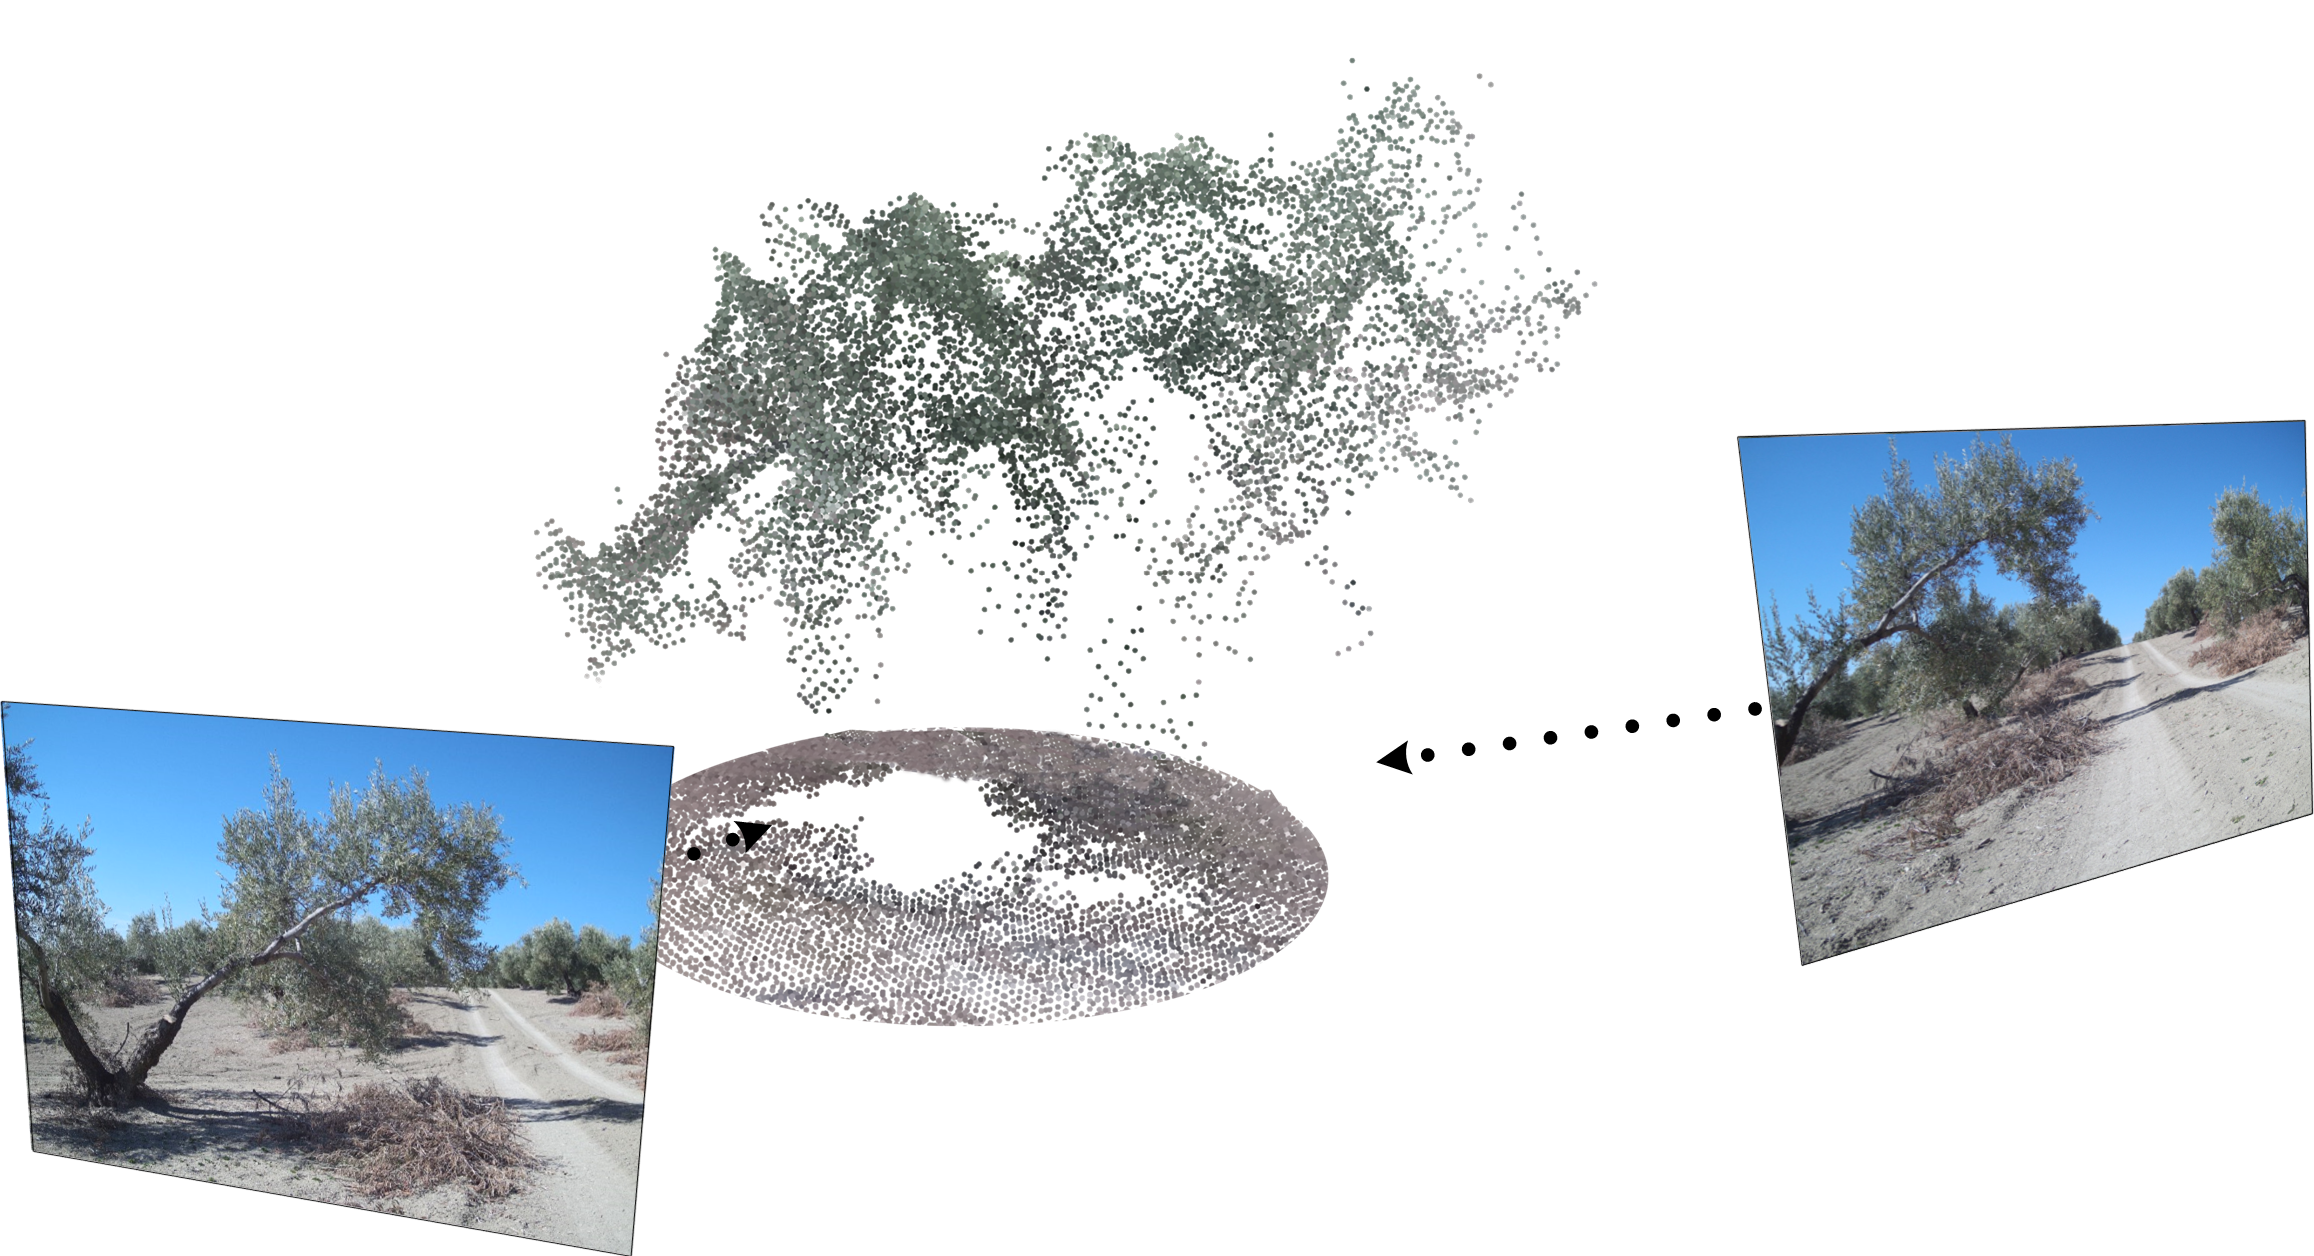
\includegraphics{figs/fundamentals/terrestrial_photogrammetry.png}
	\caption{Finding of keypoints visible in two images acquired from ground, which lead to estimating the camera pose and generating a 3D point cloud.}
	\label{fig:terrestrial_photogrammetry}
\end{marginfigure}
Photogrammetry refers to the science and technology of generating geometrically correct products derived from photographs. 3D reconstructions are fundamental in this dissertation, as they provide an automatic procedure for modelling scenes, in contrast to Computer-Aided Design (\acrshort{cad}) tools, arm-mounted probes and active methods. However, mapping is also derived from what was coined as photogrammetry: the fusion of image datasets to compound results that helps in the understanding and visualization of target areas. Some of the most common maps are Digital Surface Models (\acrshort{dsm}), Digital Terrain Models (\acrshort{dtm}) and orthophotos. These products are estimated from datasets ranging from terrestrial (Figure \ref{fig:terrestrial_photogrammetry}) and \acrshort{uas}-based imagery, which is known to be acquired sequentially in most cases, and large datasets from publicly available data. The latter images are harder to manipulate since one of their major stems is crowd-sourcing from the Internet: data published by users with very different devices, lighting conditions, visible objects in the scene, etc.

The transition from laboratory to outdoor was possible due to the advent of digital images with higher resolution, better computational capabilities and mature techniques. The overall procedure in photogrammetry is 1) to estimate parameters from cameras, 2) to reconstruct 3D points and 3) to reconstruct materials if necessary. Two slightly different techniques have had great success in recent years: Structure from Motion (\acrshort{sfm}) and Visual Simultaneous Localization and Mapping (\acrshort{vslam}), though this section is focused on the first. 

The \acrshort{sfm} method comprises a vast literature, but it has been robustly applied for over 20 years. The basis consists of 1) detecting key points in images, 2) matching these key points among multiple images, 3) estimating camera parameters from previous links and 4) building \acrshort{sfm} models. The final step, despite not being part of \acrshort{sfm}, is to reduce errors from estimations, also known as bundle adjustment (\acrshort{ba}). The error to be minimized is formally defined as follows (Equation \ref{eq:error_bundle_adjustment}) \cite{furukawa_multi-view_2015}:
\begin{gather}
    \label{eq:error_bundle_adjustment}
    \begin{aligned}
        E(P, M) = \sum_{j} \sum_{i \in V(j)} \mid P_i(M^j) - m_{i}^{j} \mid^2
    \end{aligned}
\end{gather}
where P is a set of camera parameters, ${P_i}$, $M^j$ represents a set of 3D coordinates of a track, $m_{i}^{j}$ are the projections of $M^j$ in the i-th camera, $V(j)$ are the list of cameras where a point $M^j$ is visible and $P_i(M^j)$ is the projection obtained by using the camera parameters $P_i$.

\acrshort{sfm} is also found in the literature as \acrshort{sfm}-\acrshort{mvs}, with \acrshort{mvs} referring to Multi-View Stereo. \acrshort{mvs} originated as an improvement to two-view stereo algorithms. Instead, thousands of images are applied to the reconstruction of large metropolitan and natural scenes. However, the main concerns in this regard are the photo consistency of features that are identified in several images. As we previously stated, conditions may vary from one viewpoint to another; hence, it is required to calculate how likely a candidate in $V_i$ is the correct match of a pixel in $V_j$, with $i \neq j$. Finding candidates for every feature over huge datasets is neither trivial nor efficient. Therefore, most of nowadays photogrammetric software is programmed in the \acrshort{gpu} to accelerate the pipeline.

Applying photogrammetry is not prohibitive, and it is even possible to find mobile-based applications that can work over cost- and time-efficient imagery recorded on mobile phones. Computer-based solutions, aimed at large datasets, include open-source and commercial software. The first group includes ColMap, AliceVision, Zephyr and VisualSfM, whereas notable commercial software includes Pix4DMapper \cite{zheng_thermal_2020}, Agisoft Metashape \cite{grechi_3d_2021}, RealityCapture and Autodesk Recap 360 \cite{lafi_3d_2017}. The first two commercial solutions are sped-up using multi-core \acrshort{cpu} and \acrshort{gpu} acceleration for image matching, whereas \acrshort{ba} is performed in the \acrshort{cpu}. \cite{jiang_efficient_2020} revised the efficiency of \acrshort{sfm} implementations by applying it over four datasets. According to their evaluation, performed using commodity hardware, Metashape showed the worst performance both for \acrshort{ba} and feature matching, whereas RealityCapture showed similar performance during feature matching and significantly better during \acrshort{ba}. However, Agisoft Metashape generated the densest point clouds for every dataset. Also, reported results in the literature depend on the computer used during the experiments and yet, they may vary over a short period of time. For example, Agisoft Metashape is currently known to support accelerated processing in the \acrshort{gpu} for image-matching, depth-map reconstruction and other mesh-related operations. It works over \acrshort{cuda}-enabled \acrshort{gpu}s, and therefore, it was not expected to provide results as discouraging as reported by Jiang et al. \cite{jiang_efficient_2020}.

\subsubsection{Colour aggregation}

% A final remark must be done on colour aggregations. 
Points, if back-projected to imagery, are mapped to multiple values that may vary one from another since these are captured under different lighting and viewing conditions. The observed radiance varies according to the viewing angle, expressed through azimuth, $\phi \in [0, 360]$, and zenith, $\delta \in [0, 180]$, angles. Also, surfaces behave so that the emitted radiation is not spread uniformly unless it is a perfect Lambertian generator \cite{vollmer_infrared_2017}. Surfaces emit more radiation if $\delta = 0$, i.e., the camera's view vector is $-\hat{n}$, the normal vector of the surface. The naïve and widespread way to solve aggregations is to average them \cite{javadnejad_photogrammetric_2020, hoegner_3d_2016}, while consensual approaches minimize the distance from the aggregated value to the originals. The latter method has been mainly applied to expert-guided decision-making to aggregate opinions following those operators that minimize the conflict among the experts' points of view.

Instead of averaging samples, multiple aggregation functions can be used together with penalty functions to select the aggregation that differs the less from the experts' opinions. In this context, experts are different camera viewing angles which collect distinct results. In this context, penalty functions compute the similarity of each aggregation and the starting samples \cite{bustince_definition_2017, bustince_penalty_2017}, which must be maximized (whereas the dissimilarity is minimized). Although penalty functions have been gaining interest in scientific research, they have barely been explored in some contexts such as image processing \cite{paternain_color_2012, paternain_construction_2015}. Nevertheless, they have obtained notable results on image downscaling and even upscaling.

\begin{figure}[ht]
	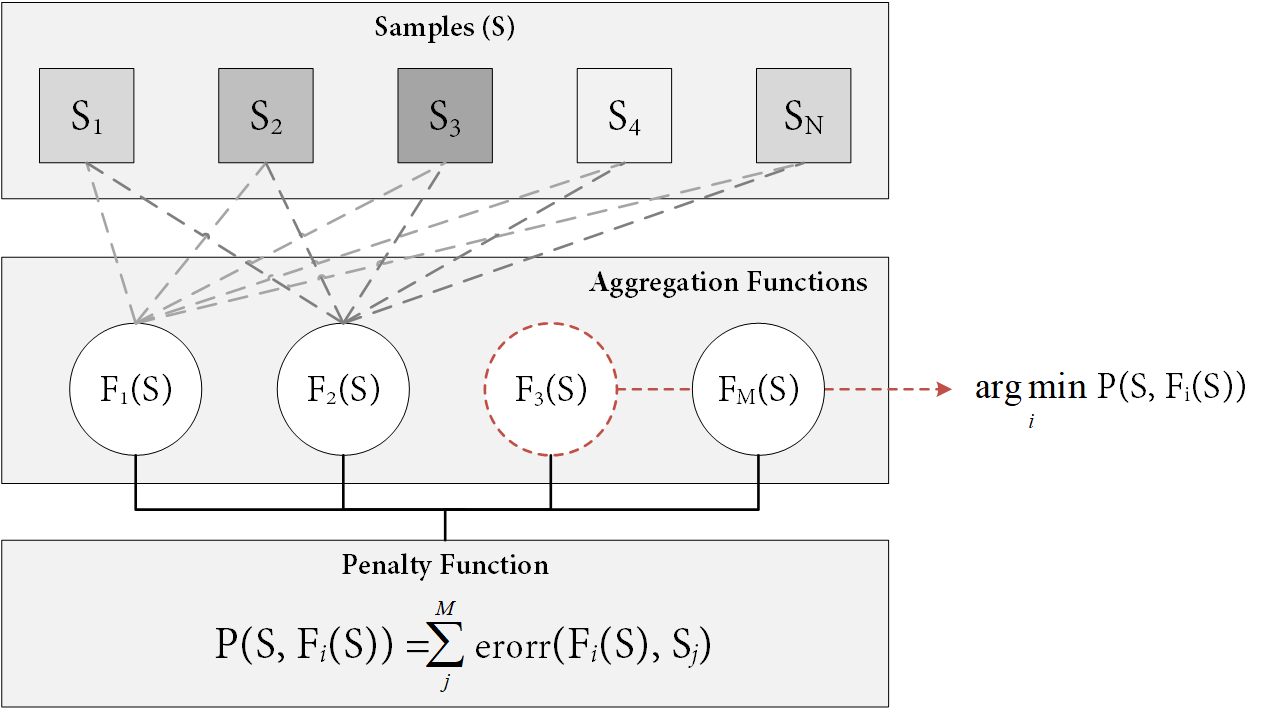
\includegraphics[width=\linewidth]{figs/fundamentals/penalty_functions.png}
	\caption{Overall procedure to compute the penalty value of every available aggregation.}
	\label{fig:penalty_funtions}
\end{figure}
Briefly, n-ary aggregation functions, $f: [0, 1]^n \rightarrow [0, 1]$ are monotone increasing and satisfy the boundary conditions (Equation \ref{eq:aggregation_boundary1}).  
\begin{gather}
    \begin{aligned}
        &\forall i \in \{1,...,n\}, \hspace{1mm} x_i \leq y\\
        &\Rightarrow f(x_1,...,x_n) \leq f(x_1,..., x_{i-1}, y, x_{i+1},...,x_n)\\
        &f(x_{\textit{min}},...,x_{\textit{min}}) = x_{\textit{min}}\\
        &f(x_{\textit{max}},...,x_{\textit{max}}) = x_{\textit{max}}
    \end{aligned}
    \label{eq:aggregation_boundary1}
\end{gather}

On the other hand, averaging aggregation functions are bounded by the minimum and maximum input (Equation \ref{eq:aggregation_boundary2}).
\begin{gather}
    \label{eq:aggregation_boundary2}
    \begin{aligned}
        \min{\{x_1,...,x_n\}} \leq f(x_1,...,x_n) \leq \max{\{x_1,...,x_n\}}
    \end{aligned}
\end{gather}

Finally, penalty functions, $P: \R^{2} \rightarrow \R$, satisfy the conditions in Equation \ref{eq:penalty_conditions}, where \textit{y} is the aggregated value. Consequently, penalty functions can be expressed as $\sum_{i=1}^{n} P(x_i, y)$ with the goal of retrieving the aggregation that minimizes the value of $P$, $g(x) \gets \operatorname*{argmin}_y P(x, y)$.
\begin{gather}
    \label{eq:penalty_conditions}
    \begin{aligned}
        &P(x_i,y) = 0 \hspace{2mm} \forall x_i = y\\
        &P(x_i,y) > 0 \hspace{2mm} \forall x_i \neq y\\
        &P(x_i,y) \ge P(x_j,y), \hspace{1mm}\mid x_i - y \mid > \mid x_j - y \mid\\
    \end{aligned}
\end{gather}

\subsubsection{Normal estimation}

Point clouds, either derived from photogrammetry or passive sensing, lack certainty in most of the attributes that provide further value to this product, ranging from normal vectors to semantic labels of different levels of detail. Many studies work on solving the uncertainty of these attributes, where normal estimation is a recurrent topic. This operation is provided as a ready-to-use tool in some widespread libraries for point cloud processing, for example, \acrshort{pcl} (Point Cloud Library) and \acrshort{cgal} (Computational Geometry Algorithms Library). Since these are very time-consuming tasks, implementations are even facilitated as multi-core solutions that significantly reduce the latency. 

Most methods addressing normal estimation operate over neighbourhoods of varying dimensionality that correlate points to form minimal triangle meshes, from which normal vectors are estimated. Thus, the main challenges in this procedure are selecting an appropriate neighbourhood size and noise resilience, as these factors greatly contribute to wrong estimations. From the neighbourhood, plane fitting is approached using unweighted Principal Component Analysis (\acrshort{pca}) and Singular Value Decomposition (\acrshort{svd}). Another challenge is the efficiency of the method: seeking the nearest $n$ points is not trivial nor efficient unless data structures with large memory footprint are built from point clouds. Hence, some works have proposed to perform a global sort on the basis of Morton codes calculated from $\textit{xyz}$ coordinates \cite{jakob_optimizing_2021}. This way, the neighbourhood is narrowed to spatially close indices on a linear buffer.

With current trends in \acrshort{ai}, normal estimation has also been achieved with Deep Learning techniques. It can be achieved by representing point clouds as graphs \cite{lenssen_deep_2020} and images \cite{zeng_deep_2019, boulch_deep_2016} since it must be performed per point rather than per voxel. To this end, additional sources of information such as depth and Hough transform \cite{boulch_deep_2016} help with the normal estimation along with $\textit{xyz}$ coordinates. 

\subsubsection{Parallel processing}

This section is focused on the revision of approaches for parallelizing processes concerning \acrshort{rs}, rather than on specific applications. The key term in this brief section is \acrshort{gpgpu}, General-Purpose computing on Graphics Processing Units, which is a programming field that takes advantage of \acrshort{gpu}s to rapidly solve parallelizable tasks. This is possible due to the large number of cores this hardware comprises. 

In this regard, \acrshort{opengl} is the most widespread Computer Graphics framework since it allows both rendering and solving computing tasks using massive geometry. From a rendering approach, point clouds have their own primitive in the draw calls, \verb|GL_POINTS|. It follows the standard rasterization pipeline while processing point clouds for rendering, despite some of these are not required for such a primitive. This drawback can be sorted out with other already explained approaches implementing a custom pipeline \cite{schutz_rendering_2021, schutz_software_2022}. For problems involving parallel computing and rendering, \acrshort{opengl} is an easy-to-use platform as it allows developers to resolve both tasks at once. However, one of the main shortcomings of \acrshort{gpgpu} in \acrshort{opengl} is the handling of asynchronous tasks that could overlap to get the most out of the \acrshort{gpu}'s capabilities, which is very limited in \acrshort{opengl} and constrained to the use of barriers. More recently, \acrshort{opengl} has been discontinued at expense of more efficient and adaptive graphics frameworks such as Vulkan, which are expected to turn into the standard frameworks in this field. Since these are still ongoing and remain niche, very few works use these platforms \cite{stumpfegger_gpu_2022}.  

Another standard framework for \acrshort{gpgpu} is \acrshort{cuda}. As opposed to \acrshort{opengl}, it is not a cross-platform tool; instead, it is only able to operate over NVIDIA \acrshort{gpu}s, but it also provides a more flexible \acrshort{gpgpu} framework. With \acrshort{opengl} being discontinued, most \acrshort{gpgpu} studies that used \acrshort{opengl} have transitioned to \acrshort{cuda} over time \cite{schutz_gpu-accelerated_2023}. Nevertheless, recent NVIDIA extensions have been introduced on both platforms. Other \acrshort{gpu}-based rendering and computing platforms are DirectX \cite{baek_accelerated_2020} (Windows OS), OpenCL (cross-platform) and Metal for Apple platforms.

\subsection{Data indexing}

This subsection introduces the reader to a shallow notion of efficient data structures for indexing point clouds and triangle meshes. This is not part of the state-of-the-art of this dissertation; instead, the aim is to understand the data structures that will be following mentioned.

This work is intended to provide scalable yet efficient products to fuse data sources and emulate them. Therefore, data structures used in ray tracing, one of nowadays most challenging \acrshort{cg} fields, are a good fit for our later implementations. Ray-tracing is mainly intended for physically-based simulations of energy spreading, with applications ranging from realistic rendering (Figure \ref{fig:ray_tracing_room}) to \acrshort{lidar} simulations and non-line-of-sight rendering aimed at finding hidden geometry \cite{royo_non-line--sight_2022}. In spite of the wide range of applications, geometry indexing in ray tracing has been mainly narrowed to Boundary Volume Hierarchies (\acrshort{bvh}) \cite{meister_survey_2021} (Figure \ref{fig:bvh_raytracing}). It is a binary tree that helps to rapidly discard parts of the scene during the traversal (half of the remaining scene with each new traversal step). Building a \acrshort{bvh} is immediate, though doing it efficiently and making later queries efficient is not as trivial. The way primitives are merged, whether a bottom-up approach is considered, has a significant impact on the traversal. The quality of a \acrshort{bvh}, once built, is measured through a cost function that estimates the minimum number of operations to find the nearest primitive. The probability of interior nodes is typically estimated with the Surface Area Heuristic (\acrshort{sah}) shown in Equation \ref{eq:sah}, which correlates the geometry of an interior node and its parent node. 
\marginnote[1cm]{
    \begin{equation}
        P(N_c|N)^{\textit{SAH}} = \frac{\textit{SA}(P(N_c))}{\textit{SA}(P(N))}
        \label{eq:sah}
    \end{equation}
}
\begin{marginfigure}[-5.0cm]
    \includegraphics{figs/fundamentals/room_rt.png}
	\caption{Ray-tracing rendering of a 3D modelled room. }
    \label{fig:ray_tracing_room}
\end{marginfigure}

\begin{figure}[ht]
	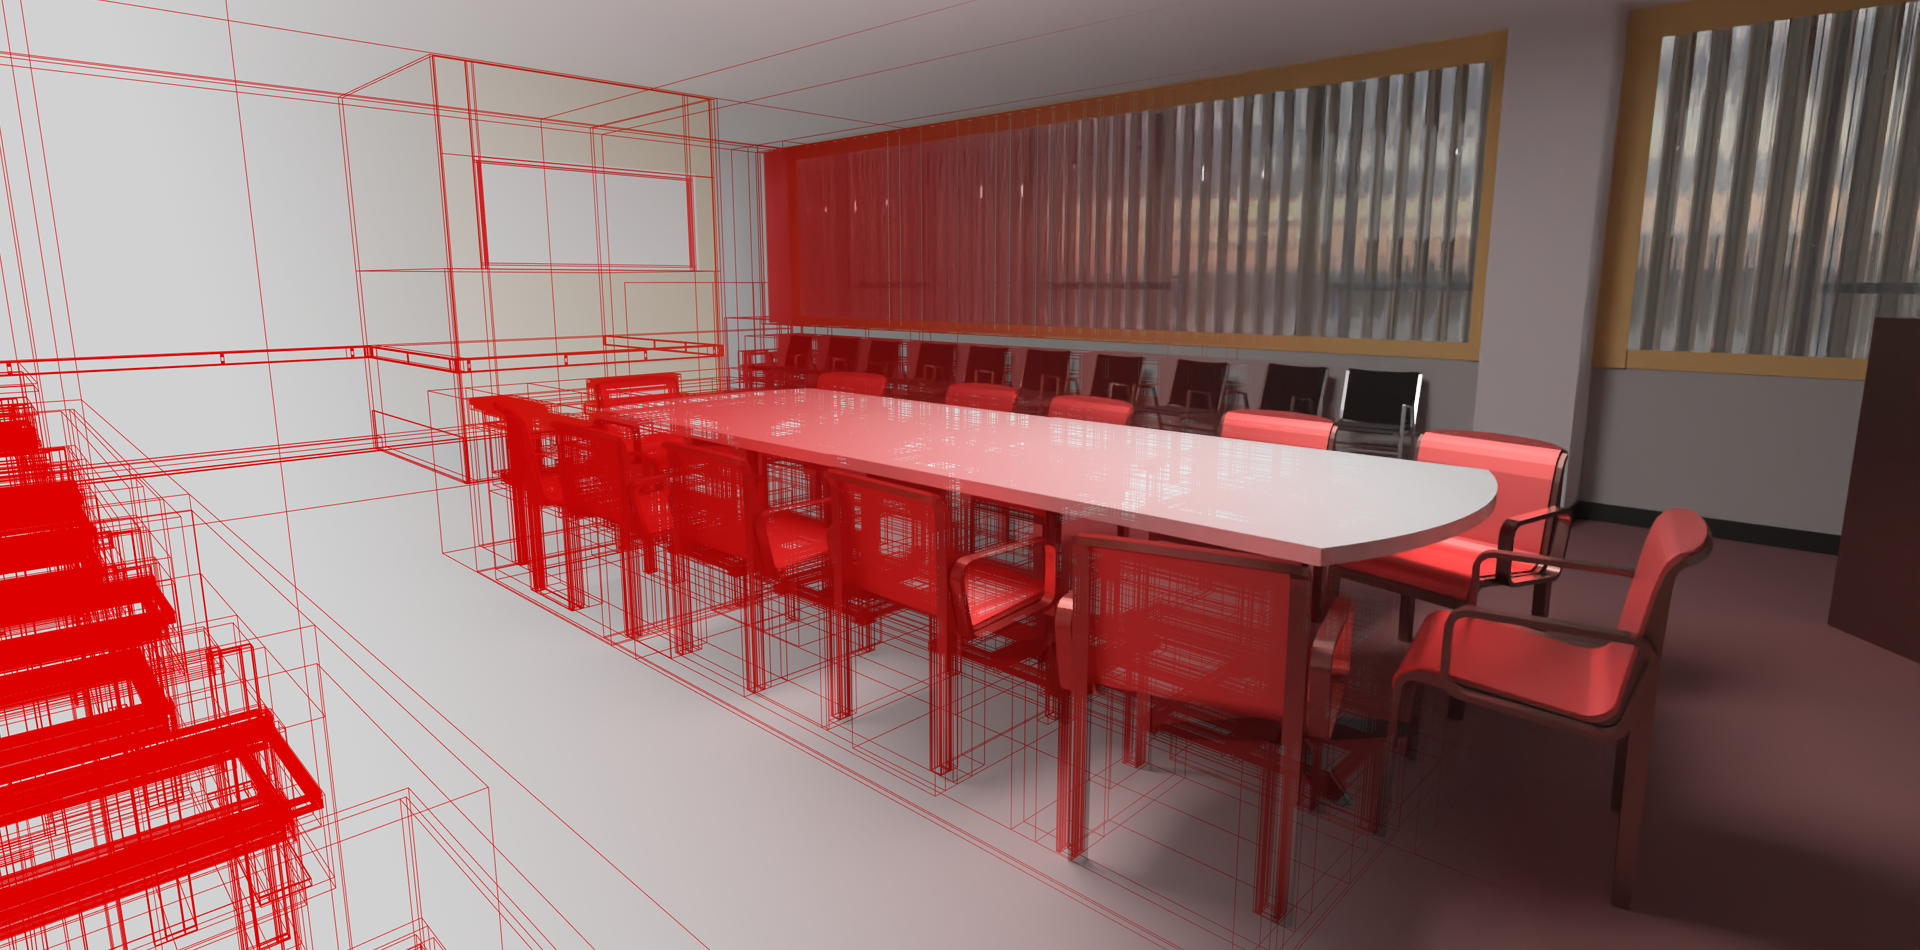
\includegraphics[width=\textwidth]{figs/fundamentals/bvh_raytracing.png}
	\caption{Rendering of the \acrshort{bvh} data structure (left side) for indexing the traditional Conference room \cite{mcguire_computer_2017} on the right side. }
    \label{fig:bvh_raytracing}
\end{figure}

\acrshort{bvh}s can either be constructed with bottom-up, top-bottom and incremental approaches. The quality of a \acrshort{bvh} cannot be estimated until completion; therefore, the merging/splitting operations are guided by heuristics. From now on, this section will be mainly explained using the algorithm of Meister and Bittner \cite{meister_parallel_2018}, which is the bottom-up construction followed in this work. The aforementioned heuristics, for instance, can be guided by the area of the bounding box enclosing two nodes for a bottom-up approach. The tighter the bounding box, the better is for later traversals. Note that larger boxes intersect a larger number of rays, thus increasing significantly the number of tests. Sometimes, however, larger boxes are intentionally preferred to avoid primitive intersection tests which are harder to resolve than ray-box collisions.

A significant challenge is to efficiently determine which are the surroundings of a primitive. It has been typically approached using what is known as Morton codes (or $Z$-curve), a data representation that encodes $x$, $y$ and $z$ coordinates with $\lfloor{\frac{2^r}{3}\rfloor}$ bits. $r \gets 5$ with 10-bit representations are the most frequent, though it can be increased to $r \gets 6$ for a higher \acrshort{lod}. This data encoding happens to sort $xyz$ points in 3D following a curve that goes through $X$, $Y$ and $Z$ axes. Therefore, a 1D buffer of Morton codes can be sorted to rapidly determine which are the neighbours of a primitive using a radius $R$. It may not return the optimal neighbour primitive for creating a new node, though it is much more efficient. Yet, $R$ can be increased at the expense of higher response time whether a better \acrshort{bvh} quality is required (if the heuristic is good enough). 

Another shortcoming is to incorporate massive parallelism in the \acrshort{gpu}. The BVH construction of Meister and Bittner \cite{meister_parallel_2018} is guided by heuristics and shortcuts in spatial searches, and yet, it is time-consuming for highly detailed scenes composed of millions of triangles (e.g., a power plant of $\sim$13M triangles has been traditionally used for comparisons \cite{mcguire_computer_2017}). However, binary-tree inspired algorithms are not a \textit{rara avis} in the \acrshort{gpu}; indeed, they are very frequently used to cope with simultaneous readings and writings in non-overlapping indices with a complexity of $\mathcal{O}(n\textit{log}(n))$. For instance, the partial summation up to each index was coined as \textit{prefix-sum} or \textit{prefix-scan}, which can be resolved in the \acrshort{gpu} with up-sweep (reduce) and down-sweep phases \cite{nguyen_gpu_2007}. Similarly, \acrshort{bvh} constructions can follow a merge and compact approach where the nearest neighbour is sought, these nodes are merged and then they are compacted in a global buffer. The \textit{prefix scan} algorithm enables the later compaction since it counts how many nodes are prior to any new node, thus determining its location in the global buffer. The response time measured for constructing the \acrshort{bvh} in \acrshort{glsl} with models ranging from 345k to 12.7M triangles is depicted in Figure \ref{fig:bvh_time}. 

\begin{figure}[ht]
    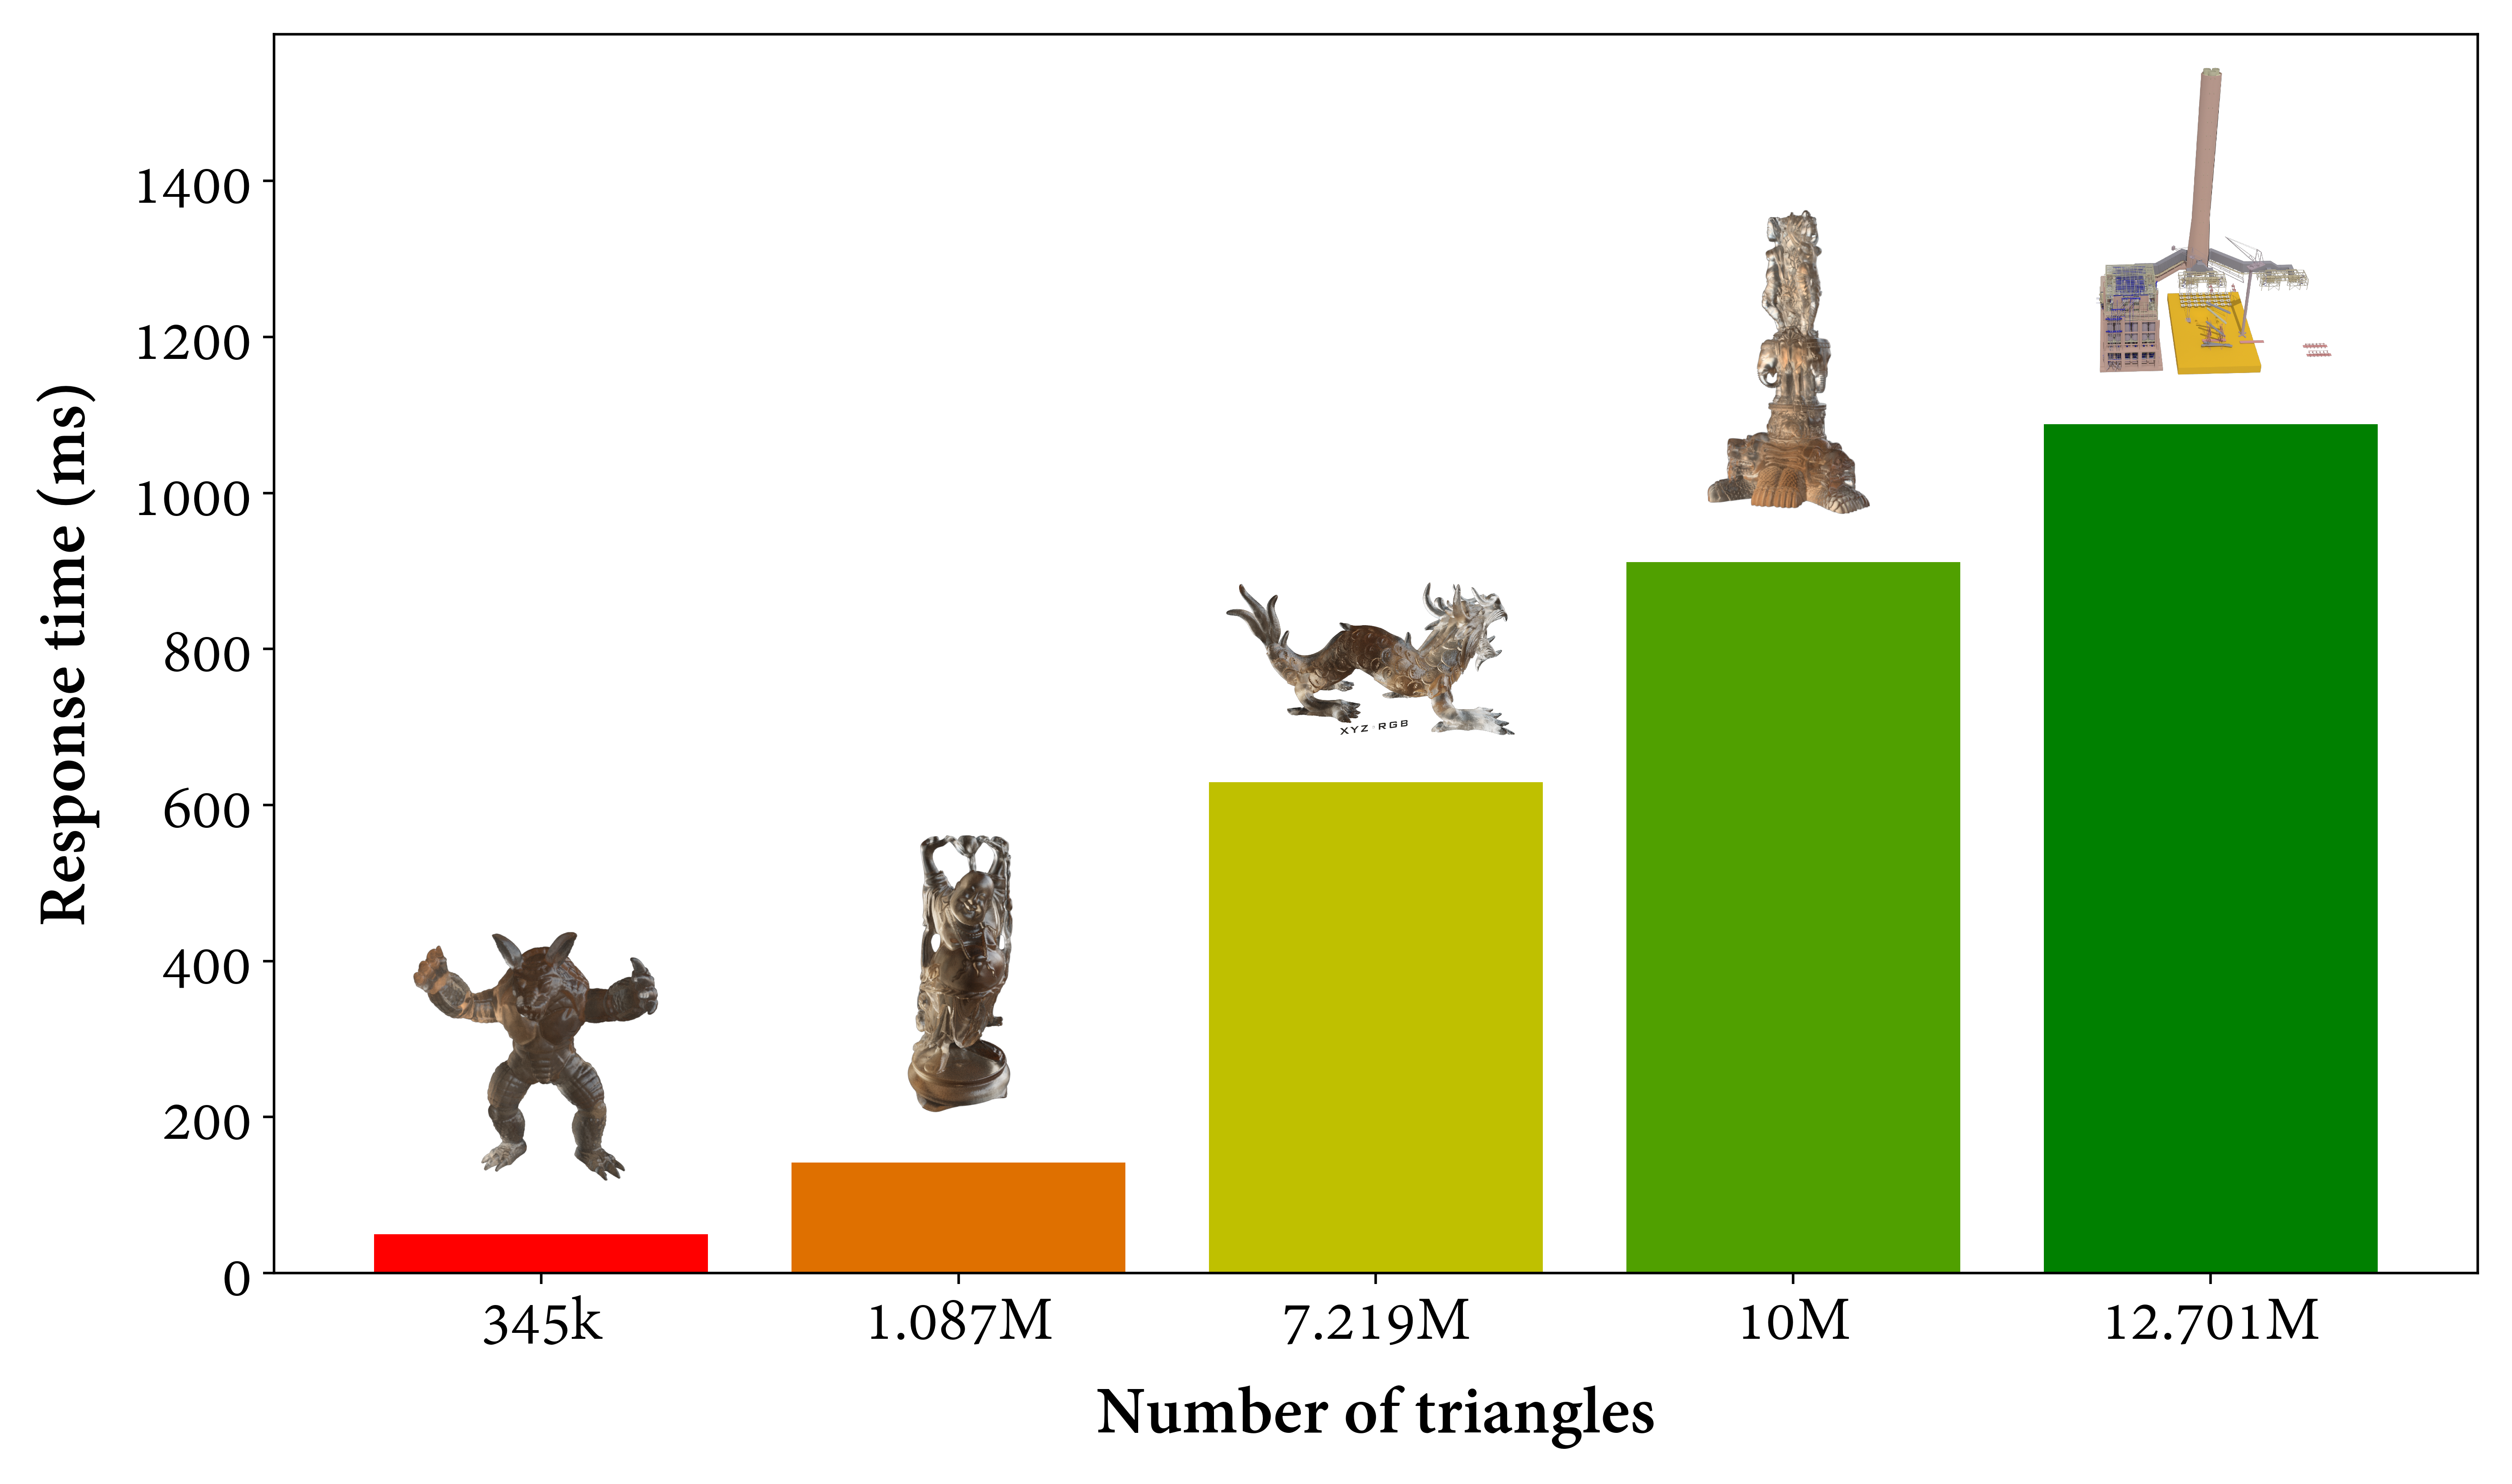
\includegraphics{figs/fundamentals/bvh_time.png}
	\caption{Response time in \si{\milli\second} required for constructing a \acrshort{bvh} for triangle meshes with a wide range of polygons. }
    \label{fig:bvh_time}
\end{figure}

One would expect the later traversals to be easier than the initial construction. Nonetheless, the first shortcoming is the looping and stack-based traversal; the first makes threads stall until the traversal is terminated, whereas the latter requires storing local access data for every thread. These shortcomings are even harder when the ray-tracing engine does not solely requires the first hit, but also any hit. Stackless traversals have been proposed, but most of them still have a small memory footprint\cite{meister_survey_2021}. It is caused by traversals requiring at least some kind of binary encoding of the path. Once footprint and traversal drawbacks are overcome, or at least mitigated to some degree, ray traversals can be further optimized by grouping rays which may have a similar outcome \cite{hendrich_ray_2019}. In this work, ray traversals were approached using a stack with local data. For millions of rays, the \acrshort{gpu} will stall for seconds as this procedure is neither efficient nor have a low memory footprint, though it is solved in much less time than would require in the \acrshort{cpu}. 

\begin{marginfigure}[-1.0cm]
    \includegraphics{figs/fundamentals/bvh_clustering.png}
	\caption{Node clustering at different \acrshort{bvh} levels. }
    \label{fig:bvh_clustering}
\end{marginfigure}
Finally, there are other data structures beyond the \acrshort{bvh} which are not as fast for ray traversals. Among them, regular grids, kd-trees and octrees are the most widespread. The first is very fast to construct ($\mathcal{O}(1)$ insertions), although it is not adaptive and queries may lead to performing a large number of ray-polygon intersection tests. It also has a great memory consumption whether a higher \acrshort{lod} is required to lower the number of intersection tests. On the other hand, octrees and kd-trees are adaptive and thus have a lower memory footprint. Subdivisions in octrees are equal splits of a bounding box, whereas kd-trees partitioning relies on the sorting of primitives along $X$, $Y$ and $Z$ axes. Hence, the former is slightly more efficient on the construction ($\mathcal{O}(\log{n})$, in contrast to the kd-tree ($\mathcal{O}(kn \log{n})$). Ray traversals have been long studied for octrees \cite{revelles_efficient_2000}, kd-trees \cite{dos_santos_kd-tree_2009} and regular grids \cite{amanatides_fast_1987} and do not represent a challenge; however, \acrshort{bvh}'s bounding boxes are tighter, i.e., the bounding box of the parent node is not equally split among its internal nodes (see Figure \ref{fig:bvh_clustering} and \ref{fig:data_structures_indexing}). The latter approach favours that fewer ray-box intersection tests are positive. Nevertheless, note that all these data structures can be constructed so that parallelism is maximized in multi-core environments, as regarded by Karras \cite{karras_maximizing_2012}.

\begin{figure*}[ht]
	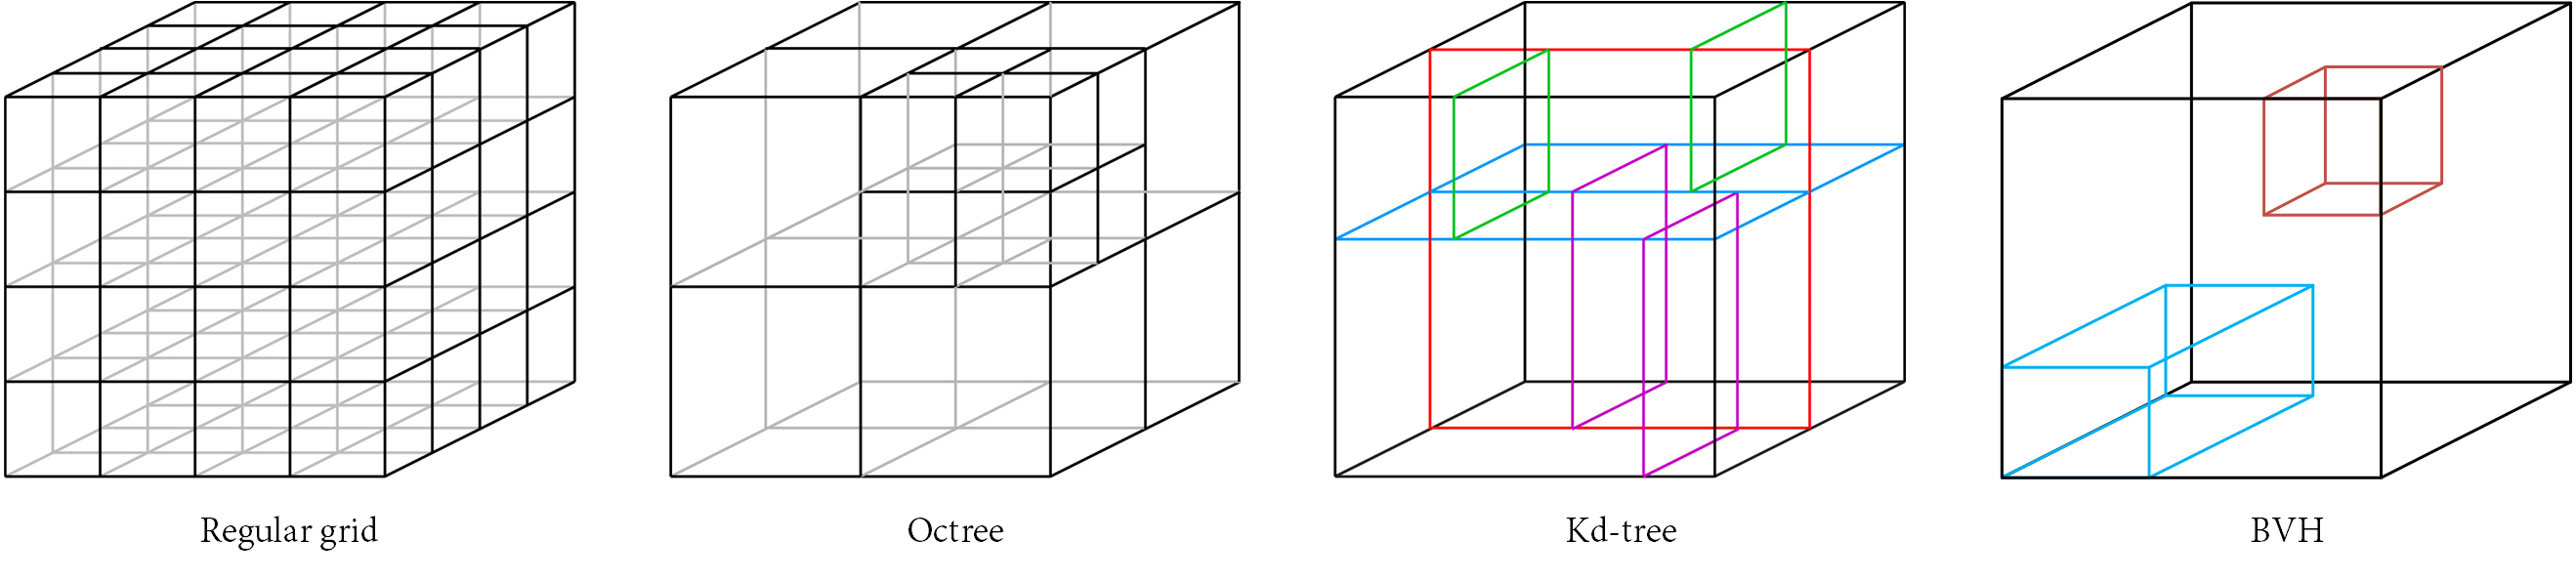
\includegraphics[width=\linewidth]{figs/fundamentals/data_structures.png}
	\caption{From left to right: regular grid, octree, kd-tree and \acrshort{bvh}. Part of the image was obtained from Ogayar et al. \cite{ogayar-anguita_nested_2023}. }
    \label{fig:data_structures_indexing}
\end{figure*}